\documentclass{beamer}
\mode<presentation>{}

\usepackage{amsmath}
\usepackage{graphicx}
\graphicspath{ {/Users/matthew.drury/Projects/model-validation/plots/} }

\AtBeginSection[]{
  \begin{frame}
  \vfill
  \centering
  \begin{beamercolorbox}[sep=8pt,center,shadow=true,rounded=true]{title}
    \usebeamerfont{title}\insertsectionhead\par%
  \end{beamercolorbox}
  \vfill
  \end{frame}
}

\DeclareMathOperator*{\argmin}{arg\,min}
\DeclareMathOperator*{\bias}{bias}
\DeclareMathOperator*{\A}{\mathcal{A}}
\DeclareMathOperator*{\F}{\mathcal{F}}
\DeclareMathOperator*{\D}{\mathcal{D}}
\DeclareMathOperator*{\T}{\mathcal{T}}
\DeclareMathOperator*{\Holdout}{\mathcal{H}}
\DeclareMathOperator*{\ESE}{\mathbf{ESE}}
\DeclareMathOperator*{\ETE}{\mathbf{ETE}}
\DeclareMathOperator*{\IESE}{\mathbf{IESE}}
\DeclareMathOperator*{\RESE}{\mathbf{RESE}}
\DeclareMathOperator*{\BIAS}{\mathbf{BIAS}}
\DeclareMathOperator*{\VAR}{\mathbf{VAR}}
\DeclareMathOperator*{\LinReg}{\text{LinReg}}	

\title{Statistical Learning Theory and Model Validation}
\author{Matthew Drury}

\begin{document}
%
\begin{frame}
  \titlepage
\end{frame}
%
\section{Introduction}
%
%
\begin{frame}
  In this talk we will discuss the error incurred when generalizing a learning
  model to unseen data.
\end{frame}
%
%
\begin{frame}
  We will see that this error comes from three distinct sources:
\end{frame}
%
%
\begin{frame}
  First is the error that results from the inherent randomness in the quantity
  being modeled.

  \begin{figure}
    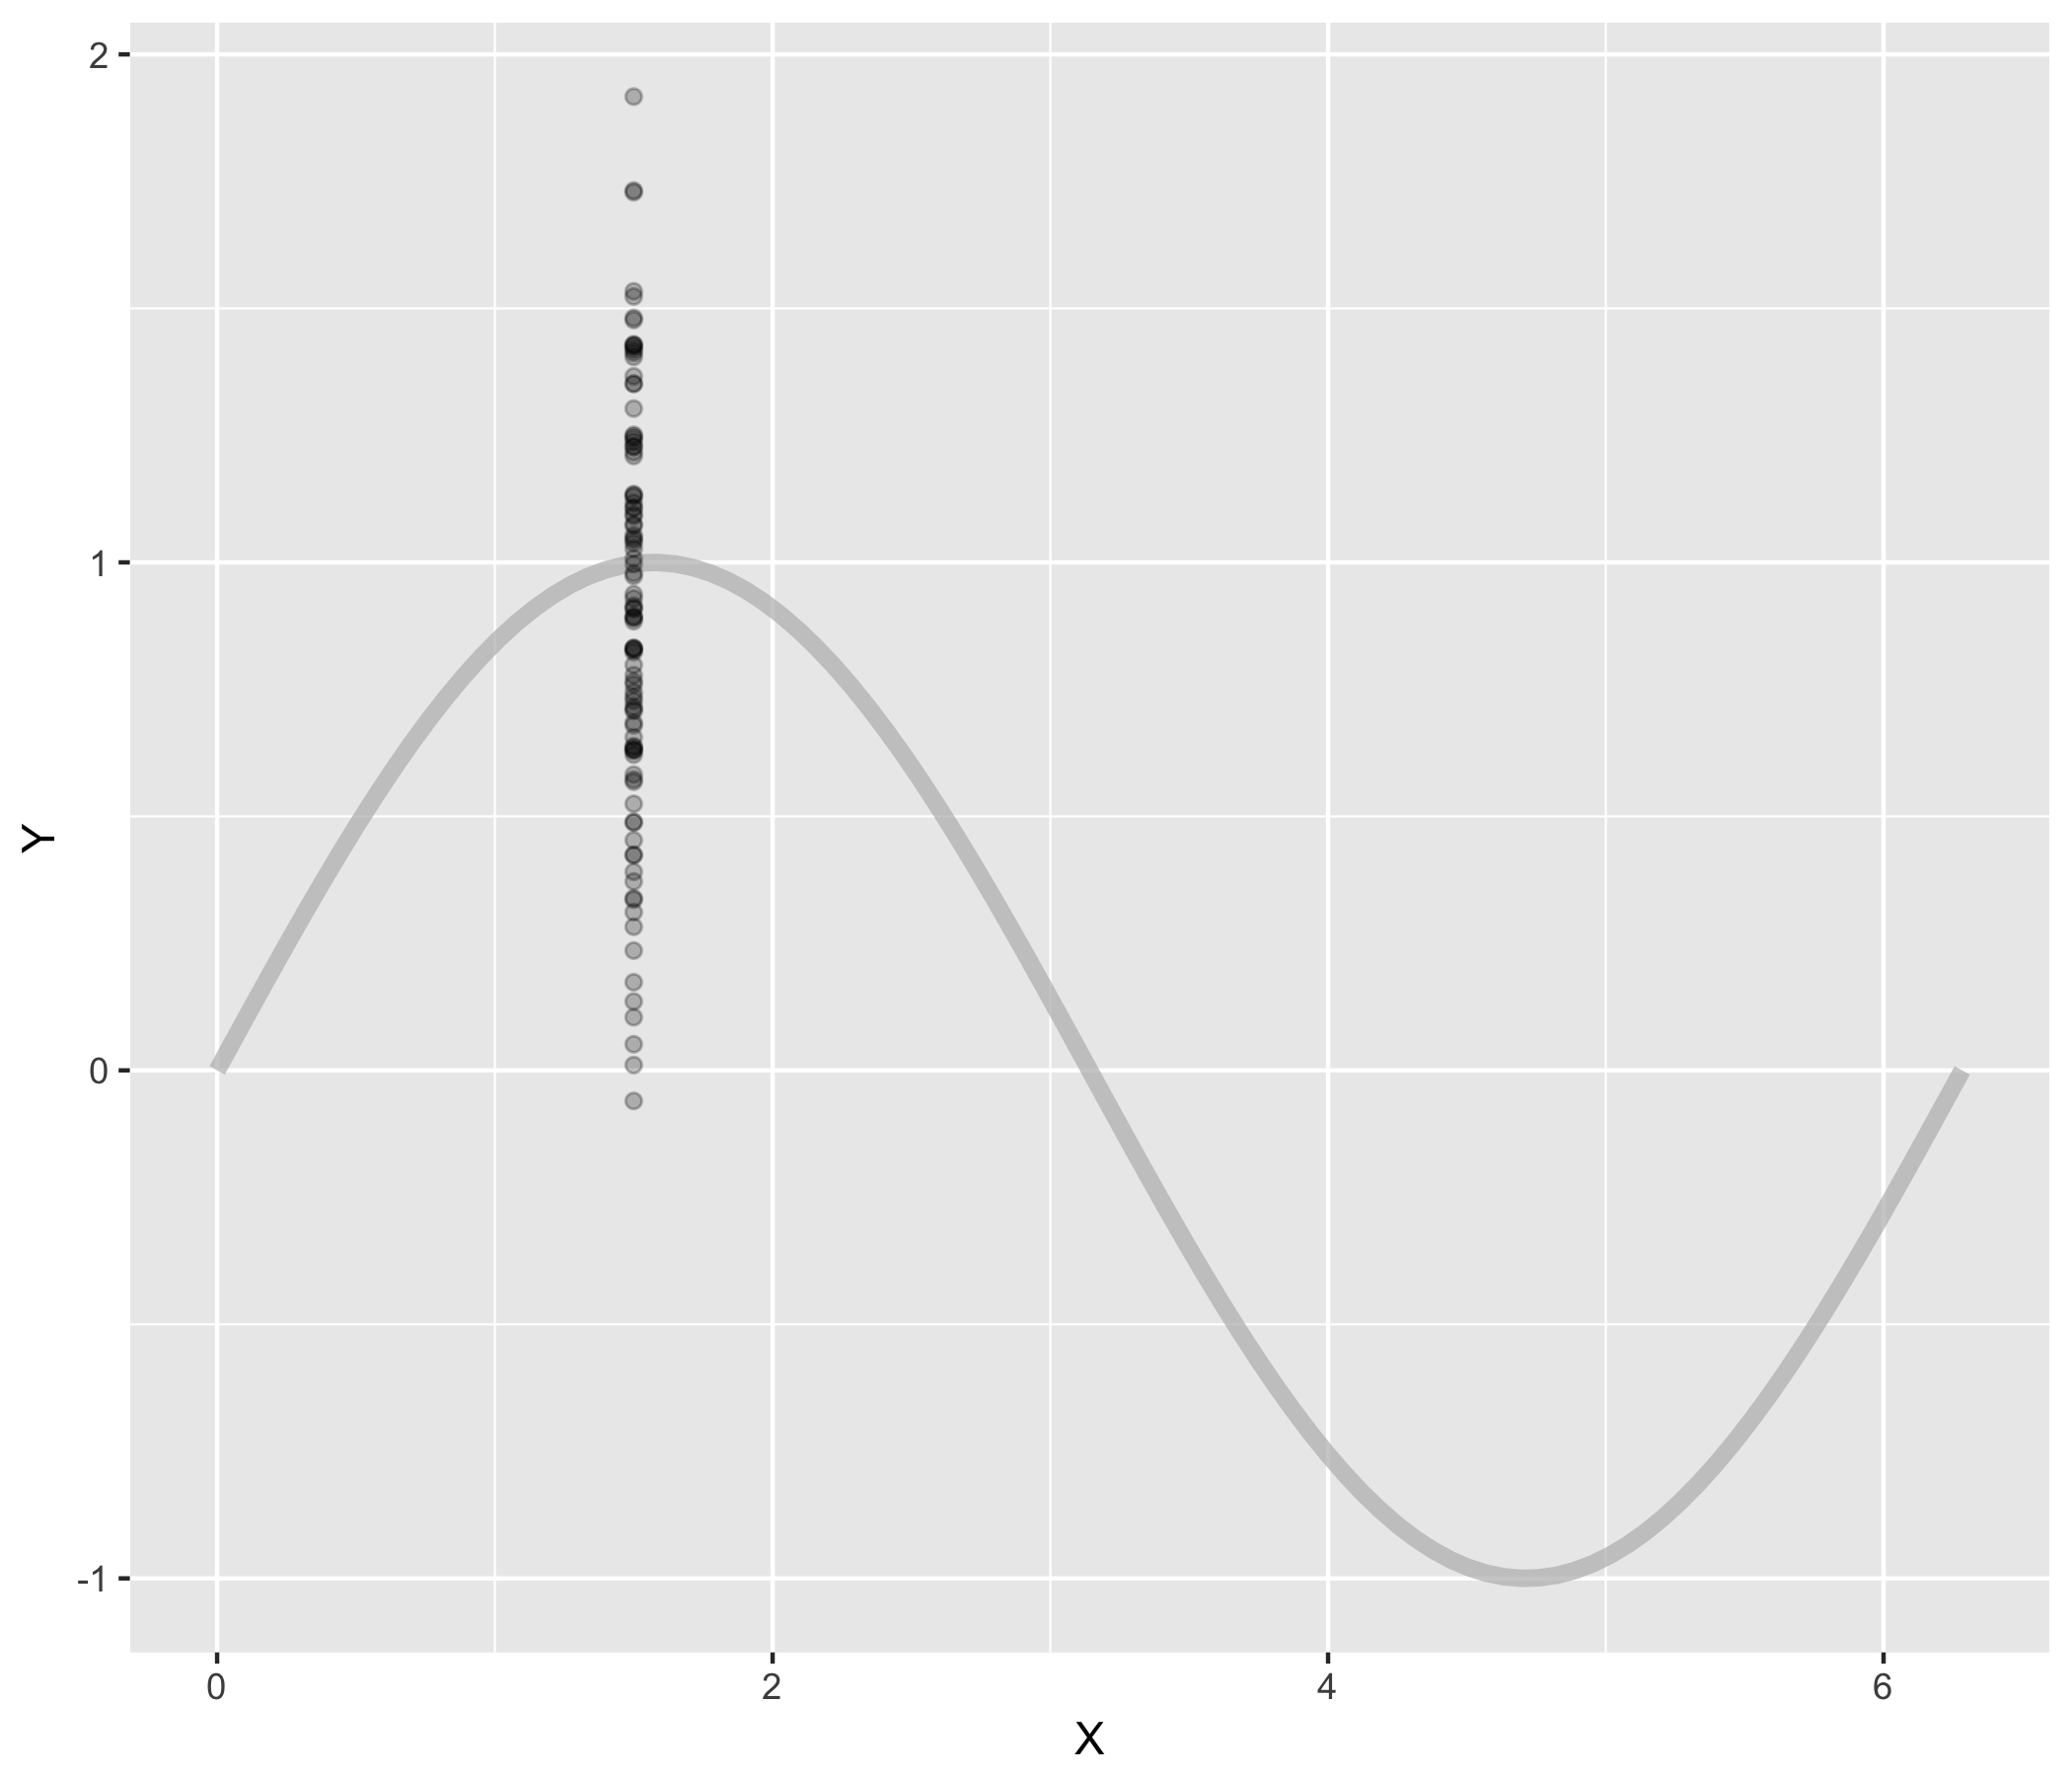
\includegraphics[scale=0.09]{irreducible_error}
  \end{figure}

  This is called the \textbf{irreducible error}
\end{frame}
%
%
\begin{frame}
  Second is the error incurred from misspecification of the model, resulting in
  an inability of the model to adapt to the target.

  \begin{figure}
    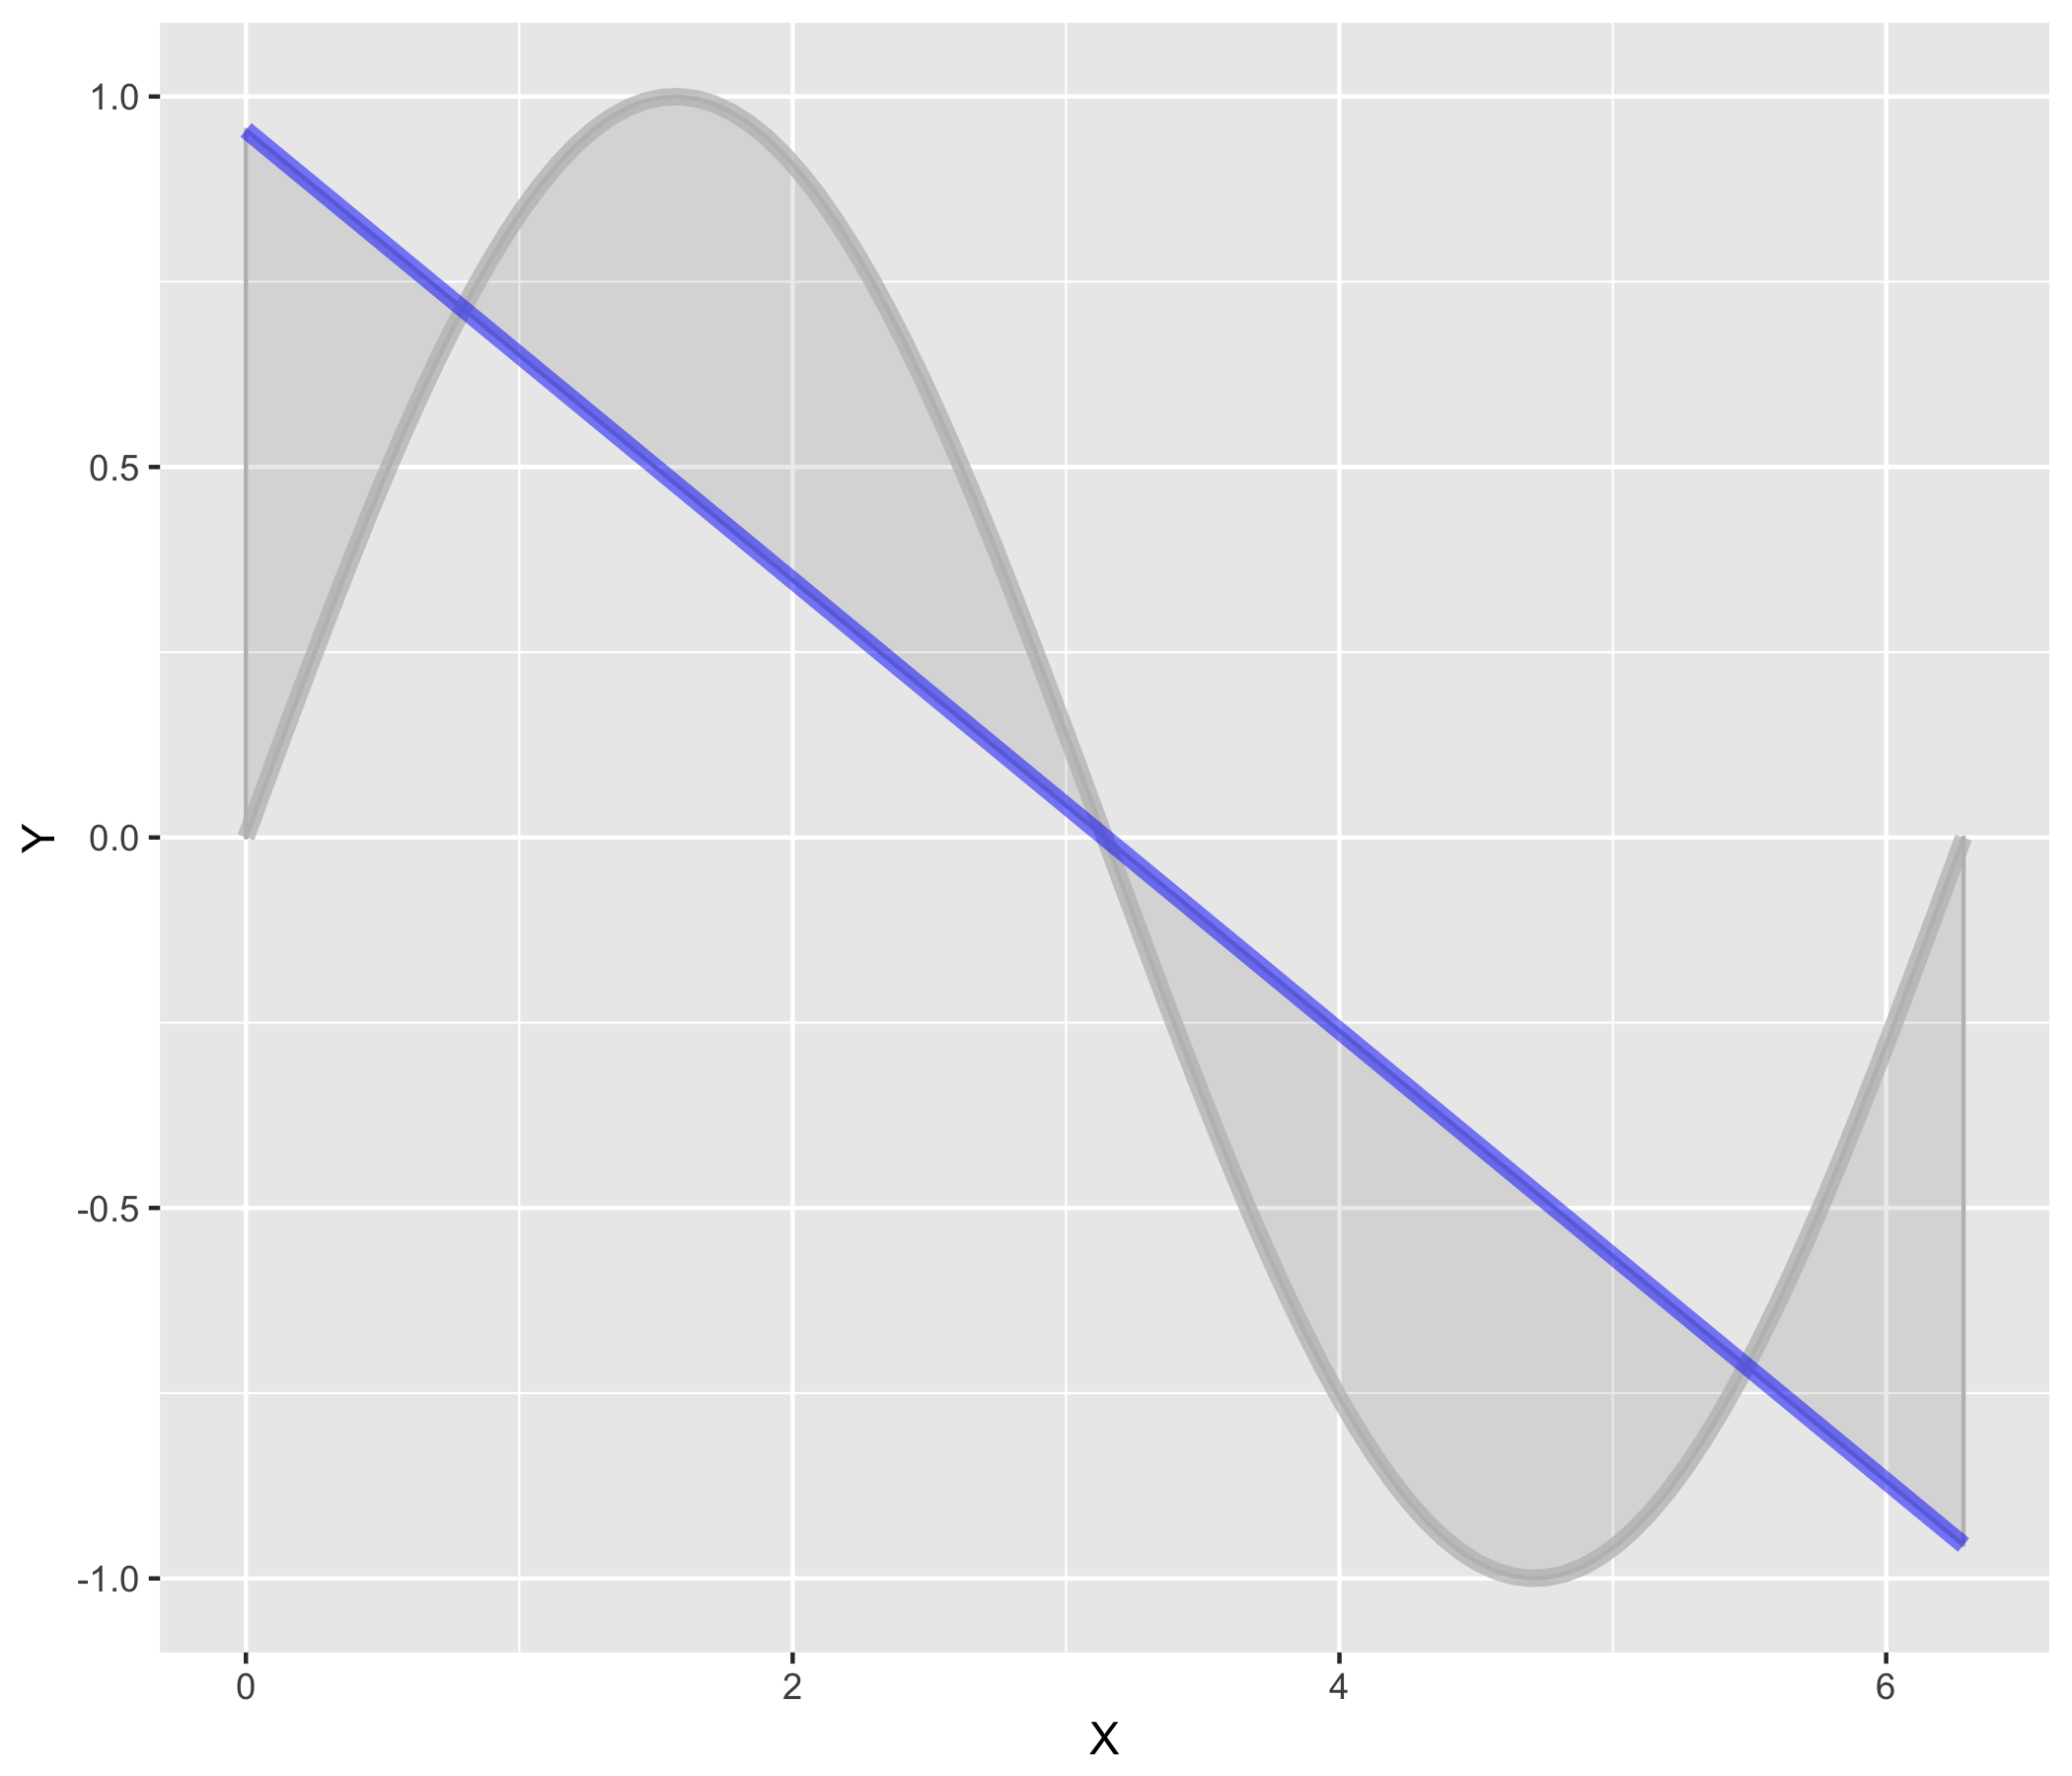
\includegraphics[scale=0.09]{model_bias}
  \end{figure}

  This is called the \textbf{model bias}.
\end{frame}
%
%
\begin{frame}
  Finally is the error incurred because our training data is not fully
  informative of random process at work, causing the model to deviate from the
  ideal fit.

  \begin{figure}
    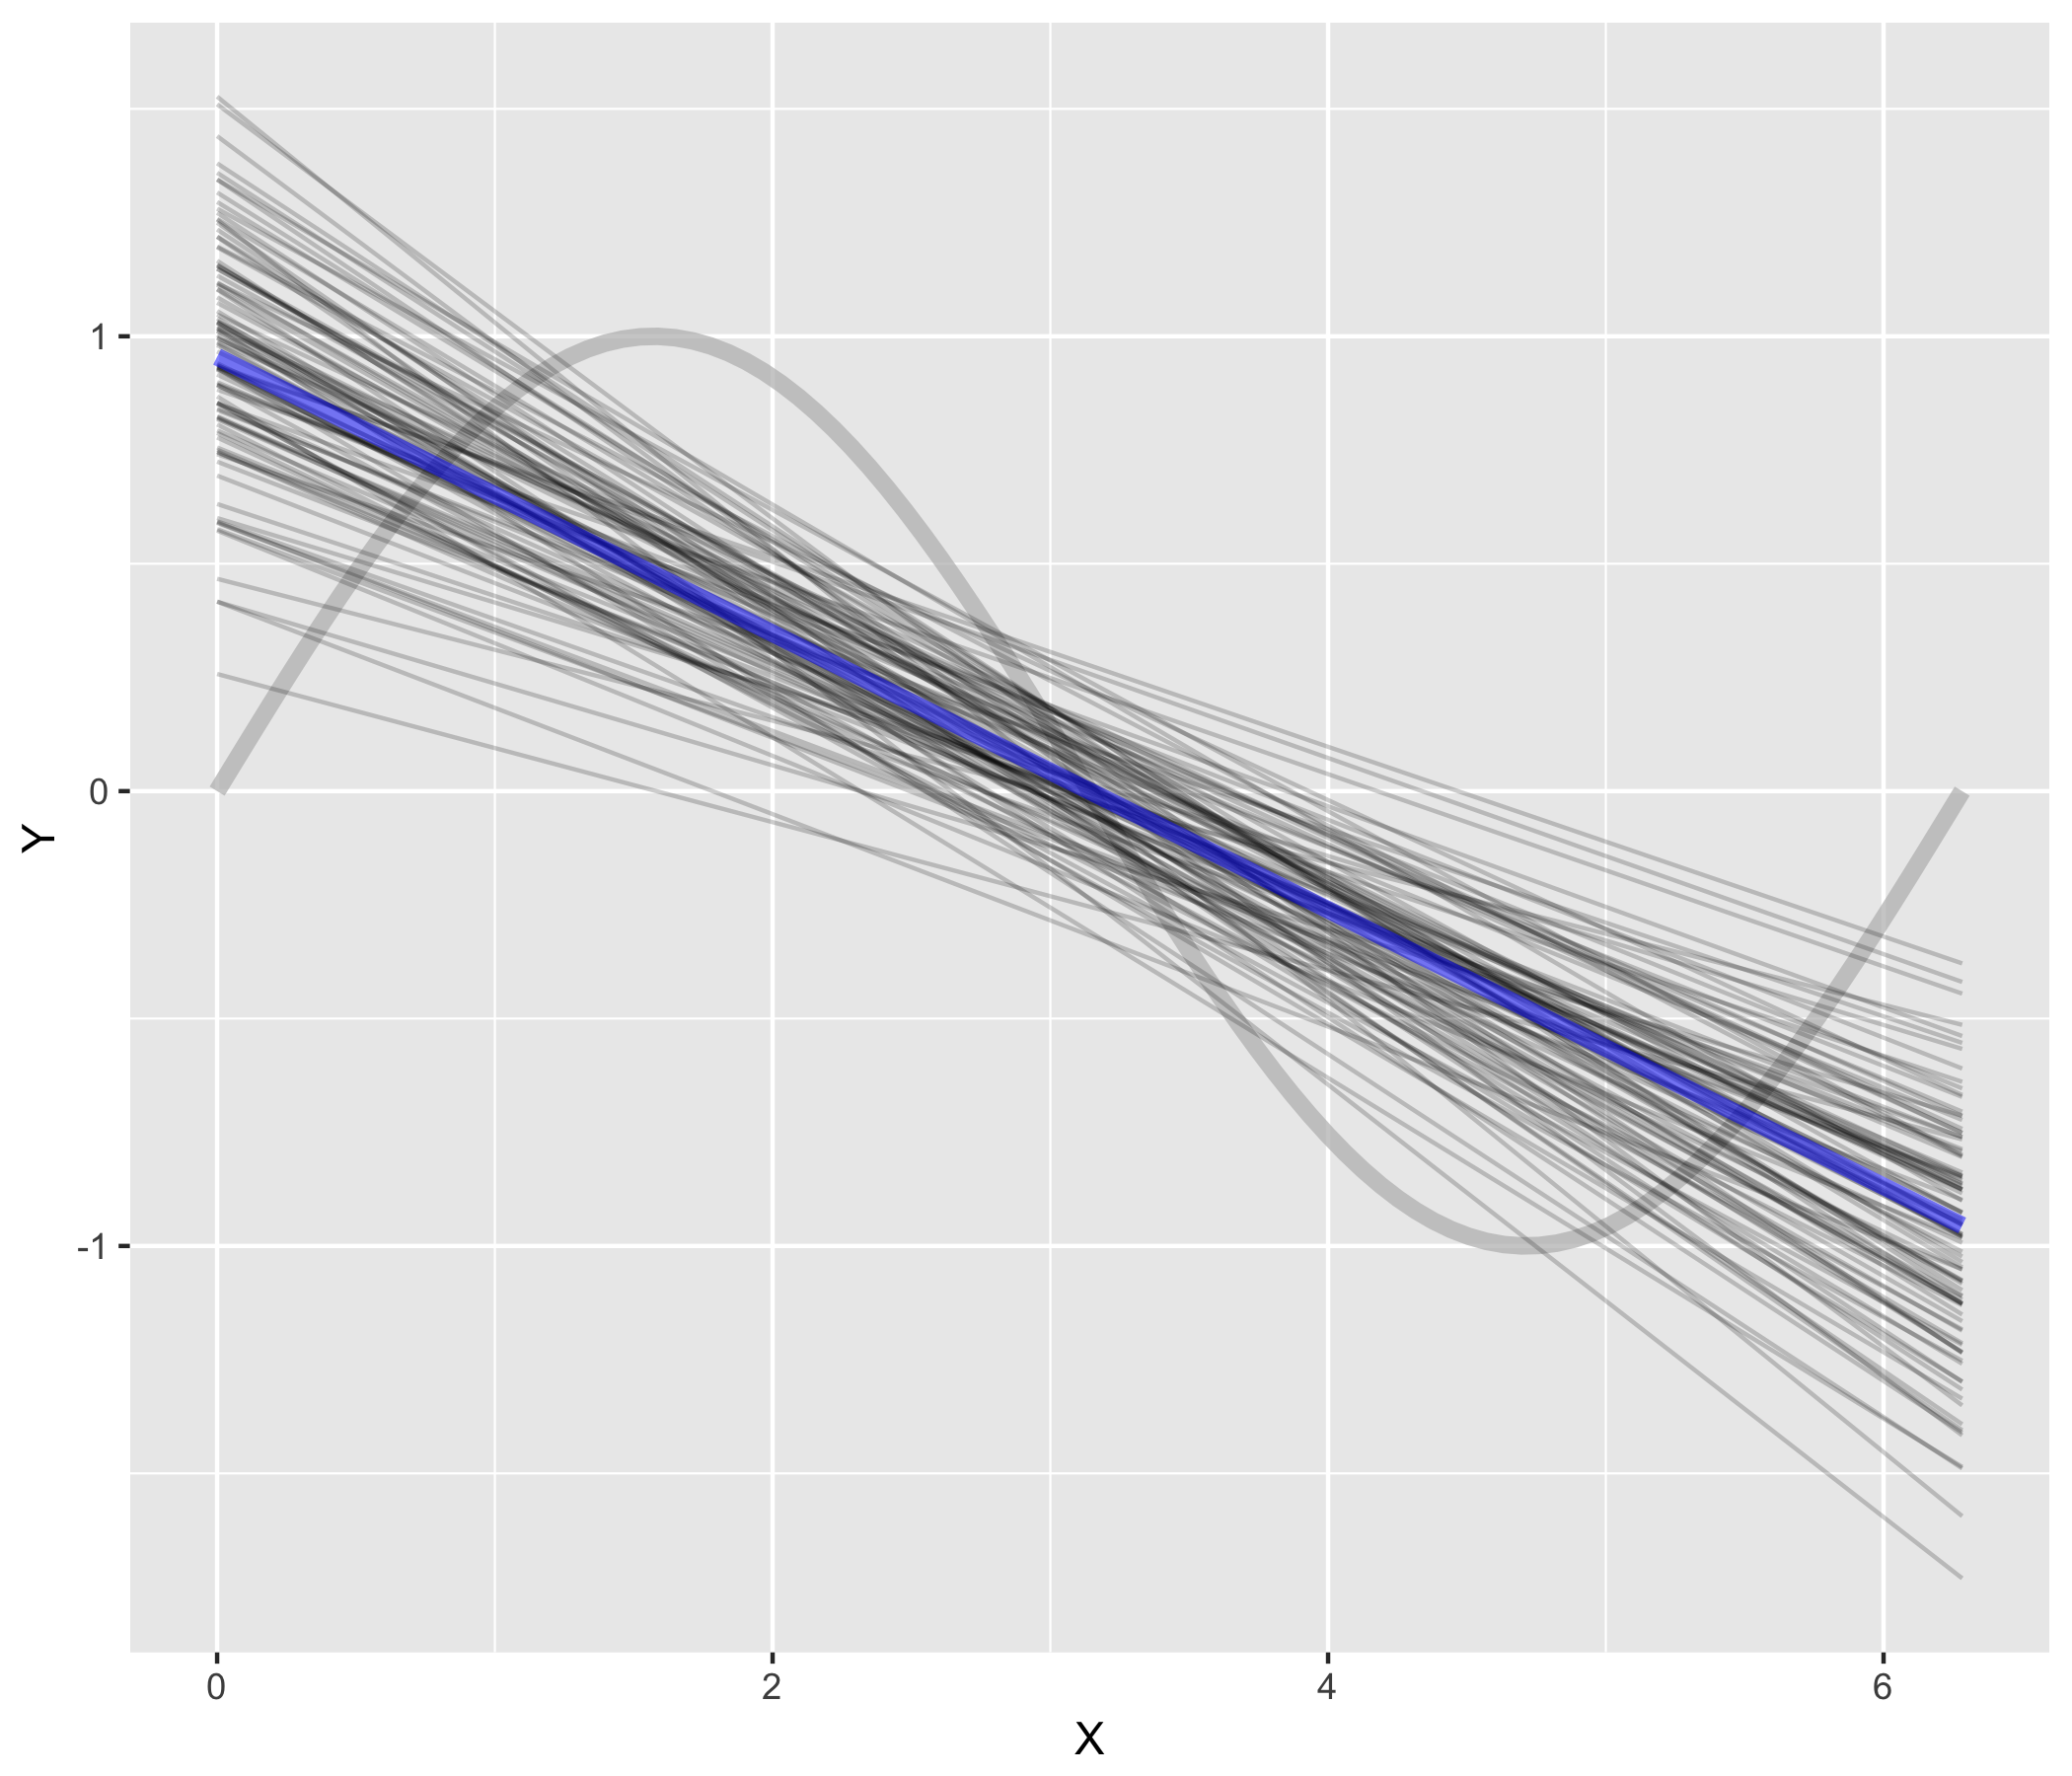
\includegraphics[scale=0.09]{model_variance}
  \end{figure}

  This is called the \textbf{model variance}.
\end{frame}

\section{A Framework for Statistical Learning}
%
%
\begin{frame}
  In this section we will outline a very general framework we can use to study
  statistical modeling.
\end{frame}
%
%
\begin{frame}
  Suppose that we have a jointly distributed random variable $X, Y$.

  The variable $X$ is called the \textbf{predictor}.

  The variable $Y$ is called the \textbf{response}.
\end{frame}
%
%
\begin{frame}
  In general, we think of the distribution of $X$ as unknowable, and our goal is
  to learn something about the conditional distribution $Y|X$.
\end{frame}
%
%
\begin{frame}
  The simplest thing we could want to know is the expectation $E(Y|X)$, which is
  a pure function of $X$, and is often referred to as the \textbf{regression
  function}.
\end{frame}
%
%
\begin{frame}
  An attractive method for estimating approximations to the regression function
  is to minimize some \textbf{loss functional} chosen so that the minimizer is
  ``close'' to the regression function.
\end{frame}
%
%
\begin{frame}
  The most popular choice is the \textbf{squared error loss}.  
  
  $$ \ESE(f) = E_{X, Y} \left[ (y - f(x))^2 \right] $$

  which is ubiquitous for good reason: the pointwise minimizer of
  
  $$ \ESE(f; x) = E_Y \left[ (y - f(x))^2 \mid x \right] $$
  
  \textbf{is} the regression function.
\end{frame}
%
%
\begin{frame}

  % Demonstration that the regression function minimizes the expected 
  % squared error.
  \begin{align*}
    \ESE(f; x)& = E_Y \left[ \left( y - \textcolor<8>{blue}{f(x)} \right)^2 \mid x \right] \\
    %Squaring
    \onslide<2->{
      & = E_Y \left[ \left( y - \textcolor<2>{orange}{E[y \mid x] + E[y \mid x]} 
          - f(x) \right)^2 \mid x \right] \\
    }
    % Outside terms
    \onslide<3->{
      & = E_Y \left[ \left( y - E[y \mid x] \right)^2 \mid x \right] 
          + E_Y \left[ \left(E[y \mid x] - f(x) \right)^2 \mid x \right] \\
    }
      % Inside square term
      \only<3-5> {
      & \quad + 2 E_Y \left[ 
          \textcolor<5>{orange}{ \left( y - E[y \mid x] \right) } 
          \textcolor<4>{orange}{ \left( E[y \mid x] - f(x) \right) } 
        \mid x \right] \\
      }
    % Discarding the positive term...
    \onslide<7->{
      & \geq E_y \left[ \left( y - \textcolor<8>{blue}{E[y \mid x]} \right)^2 \mid x \right]
    }
  \end{align*}

  % Notes on the computation.
  \only<2>{The most common trick in mathematics: add zero.}
  \only<3>{Square.}
  \only<4>{This factor has no dependence on y, so it is a constant from the view of the outside expectation.}
  \only<5>{This factor is zero in expectation, so the cross term is zero.}
  \only<6>{Goodbye!}
  \only<7>{Discarding a positive term.}
  \only<8>{The regression function $E[Y|X]$ is the minimizer.}

\end{frame}
%
%
\begin{frame}
  Because of it's importance, let's reserve the symbol $\F$ for the regression
  function:

  $$\F(x) = E_Y \left[ Y | X \right]$$
  
  It is also common to refer to $\F$ as the \textbf{ground truth}, just the
  \textbf{truth}, or the \textbf{signal}.
\end{frame}
 % A Framework for Statistical Learning
\section{The Bias-Variance Decomposition}
%
%
\begin{frame}
  Although we never have full knowledge about $X, Y$, we often do have sample
  data drawn from this distribution:

  $$ \D = \left\{ (x_i, y_i) \mid x_i, y_i \sim X, Y \right\} $$
\end{frame}
%
%
\begin{frame}
  Approximating $\F$ often takes the form of a \textbf{learning algorithm}:

  $$ \A : \D \mapsto f $$

  which, given a sample dataset $\D$, produces a function $f$ that approximates
  $\F$.
\end{frame}
%
%
\begin{frame}
  A learning algorithm induces an extremely enlightening decomposition of the
  expected squared error. This is called the \textbf{bias-variance}
  decomposition.
\end{frame}
%
%
\begin{frame}

  \only<1>{
    Recall our decomposition of the expected squared error from the previous
    section:
  }

  % Decomposition of expected squared error into irreducible and modelable
  % error.
  \begin{align*}
    \ESE(f; x) & = E_Y \left[ \left( y - f(x) \right)^2 \mid x \right] \\
      & = \textcolor<2>{orange}{
        E_Y \left[ \left( y - \F(x) \right)^2 \mid x \right]
      } 
      + \textcolor<3-4>{orange}{
          \only<1-3>{ E_Y \left[ }
            \left( \F(x) - f(x) \right)^2
          \only<1-3>{ \mid x \right] }
      }
  \end{align*}

  \only<2>{
    This term cannot be reduced by a learning algorithm, it measures the
    variance of $Y$ about its mean.  This is called the \textbf{irreducible
    error}
  }
  \only<3>{
    This term does not depend on $Y$, and so the expectation can be discarded. 
  }
  \only<4>{
    We can reduce this term by choosing $f$ well, and it is the goal of the
    learning algorithm to make this term as small as possible.  We call it the
    \textbf{reducible error}.
  }

\end{frame}
%
%
\begin{frame}
  $$ \IESE(x) = E_Y \left[ \left( y - \F(x) \right)^2 \mid x \right] $$
  $$ \RESE(f; x) = \left( \F(x) - f(x) \right)^2 $$
\end{frame}
%
%
\begin{frame}
  The second term in the previous equation can be further decomposed, but to do
  so we will have to introduce a new concept.  
\end{frame}
%
%
\begin{frame}
  Recall that $f$ depends on the data set $\D$ through our learning algorithm:

  $$ \A : \D \mapsto f $$

  We can make this dependence explicit by writing $f(x; \D)$.
\end{frame}
%
%
\begin{frame}
  The datasets $\D$ (of a fixed size) can be thought of as being drawn from
  their own distribution, the \textbf{sampling distribution} of $X$.   
\end{frame}
%
%
\begin{frame}
  We would like to study how the expected error of our predictions depends on
  the randomness in $\D$:

  $$ \ESE(f; x) = E_{Y,\D} \left[ \left( y - f(x; \D) \right)^2 \mid x \right]
  $$

  Note that the previous decomposition into irreducible and reducible error
  still holds for this expectation, as our calculations made no assumptions
  about $f$.
\end{frame}
%
%
\begin{frame}
  To break down the reducible error, we introduce the expectation of $f$ with
  respect to the data $\D$:

  $$ Ef(x) = E_{\D} \left[ f(x, \D) \mid x \right] $$
\end{frame}
%
%
\begin{frame}
  \begin{align*}
    \RESE & (f; x) \\
    &= E_{D} \left[ \left( \F(x) - f(x,\D) \right)^2 \mid x \right]
    \\
    %Squaring
    \onslide<2->{
      & = E_{\D} \left[ \left( \F(x) - \textcolor<2>{orange}{Ef(x) + Ef(x)} 
          - f(\D) \right)^2 \mid x \right] \\
    }
    % Outside terms
    \onslide<3->{
      & = \textcolor<6>{orange}{
             \only<3-6>{ E_{\D} \left[ } 
               \left( \F(x) - Ef(x) \right)^2 
             \only<3-6>{ \mid x \right] }
           }
           + E_{\D} \left[ \left(Ef(x) - f(x,\D) \right)^2 \mid x \right] \\
    }
      % Inside square term
      \only<3-5> {
      & \quad + 2 E_{\D} \left[ 
          \textcolor<4>{orange}{ \left( \F(x) - Ef(x) \right) } 
          \textcolor<5>{orange}{ \left( Ef(x) - f(x,\D) \right) } 
        \mid x \right] \\
      }
  \end{align*}

  \only<2>{Add zero.}
  \only<3>{Square.}
  \only<4>{This factor has no dependence on $\D$, so it is a constant from
  the view of the enclosing expectation.}
  \only<5>{This factor is zero in expectation, so the cross term is zero.}
  \only<6>{This term has no dependence on $\D$, so we can remove the
  expectation.}
  \only<7>{This is the \textbf{bias-variance decomposition.}}

\end{frame}
%
%
\begin{frame}
  \begin{align*}
    \RESE & (f; x) \\
      & = \textcolor<1>{orange}{
            \left( \F(x) - Ef(x) \right)^2
          }
          + 
          \textcolor<2>{orange}{
            E_{\D} \left[ \left( Ef(x) - f(x,\D) \right)^2 \mid x \right]
          }
  \end{align*}
%
  \only<1>{
    This is the \textbf{model (squared) bias}, which measures the deviation of
    the algorithm's average result approximation from the ground truth.
  }
  \only<2>{
    This is the \textbf{model variance}, which measures the variance of the
    algorithm's results around its average result.
  }
\end{frame}
%
%
\begin{frame}
  \begin{align*}
    \BIAS (x)^2 = \left( \F(x) - Ef(x) \right)^2
  \end{align*}

  The model bias tends to be decrease as the learning algorithm becomes more complex,
  and increase as it becomes more rigid. 
\end{frame}
%
%
\begin{frame}
  \begin{align*}
    \VAR(x) = E_{\D} \left[ \left( Ef(x) - f(x,\D) \right)^2 \mid x \right]
  \end{align*}

  The model variance tends to increase as the learning algorithm becomes more
  complex, and decrease as it becomes more rigid.
\end{frame}
%
%
\begin{frame}
  It is possible to make the phrases ``learning algorithm becomes more/less complex''
  precise, but it is not easy, and it will have to wait for another talk.
\end{frame}
%
%
\begin{frame}
  Here is our final decomposition of the expected squared error into various
  sources of error:

  \begin{align*}
    \ESE & (f; x) \\
    &= \color{blue}{ 
         E_Y \left[ \left( y - E_Y[y \mid x] \right)^2 \mid x \right] } \\
       & \quad + \color{red}{
         \left( E_Y[y \mid x] -  E_{\D} \left[ f(x, \D) \mid x \right] \right)^2
       } \\
       & \quad + \color{green}{
         E_{\D} \left[ \left( E_{\D} \left[ f(x, \D) \mid x \right] - 
         f(x,\D) \right)^2 \mid x \right]
       }
  \end{align*}
  \begin{center}
    \color{blue}{Irreducible Error} - \color{red}{Model Bias} - \color{green}{Model
    Variance}
  \end{center}
\end{frame}
%
%
\begin{frame}
  So far, we have concentrated on the \textbf{pointwise} error rates $\ESE(x)$.
  Often time, we concern ourselves with the \textbf{overal} error rates, which
  are found by taking the expectation with respect to $X$ as well:

  \begin{align*}
    \ESE(f) & = E_{X,Y} \left[ \left( y - f(x) \right)^2 \right] \\
    &= E_X E_{Y \mid X} \left[ \left( y - f(x) \right)^2 \mid x \right]
  \end{align*}

  Discussions of this nature can often become confusing if you do not keep in
  mind whether the \textbf{overall} of \textbf{pointwise} error is being
  considered.  We will try to be explicit.
\end{frame}
 % The Bias-Variance Decomposition
\section{A Toy Model}
%
%
\begin{frame}
  So far we have worked out a sound theoretical foundation to understand the
  errors incurred when building learning algorithms.  In this section we will
  analyze in detail how these concepts look with a toy model.
\end{frame}
%
%
\begin{frame}
  Our data generating process will be very simple so that we can fully analyse
  the situation:

  \begin{align*}
    X &\sim U(0, 2 \pi) \\
    Y &\sim \sin(X) + N(0, \epsilon)
  \end{align*}

  Where $U$ is the uniform distribution on an interval, and $N$ is the normal
  distribution with a given mean and variance.
\end{frame}
%
%
\begin{frame}
  \begin{figure}
    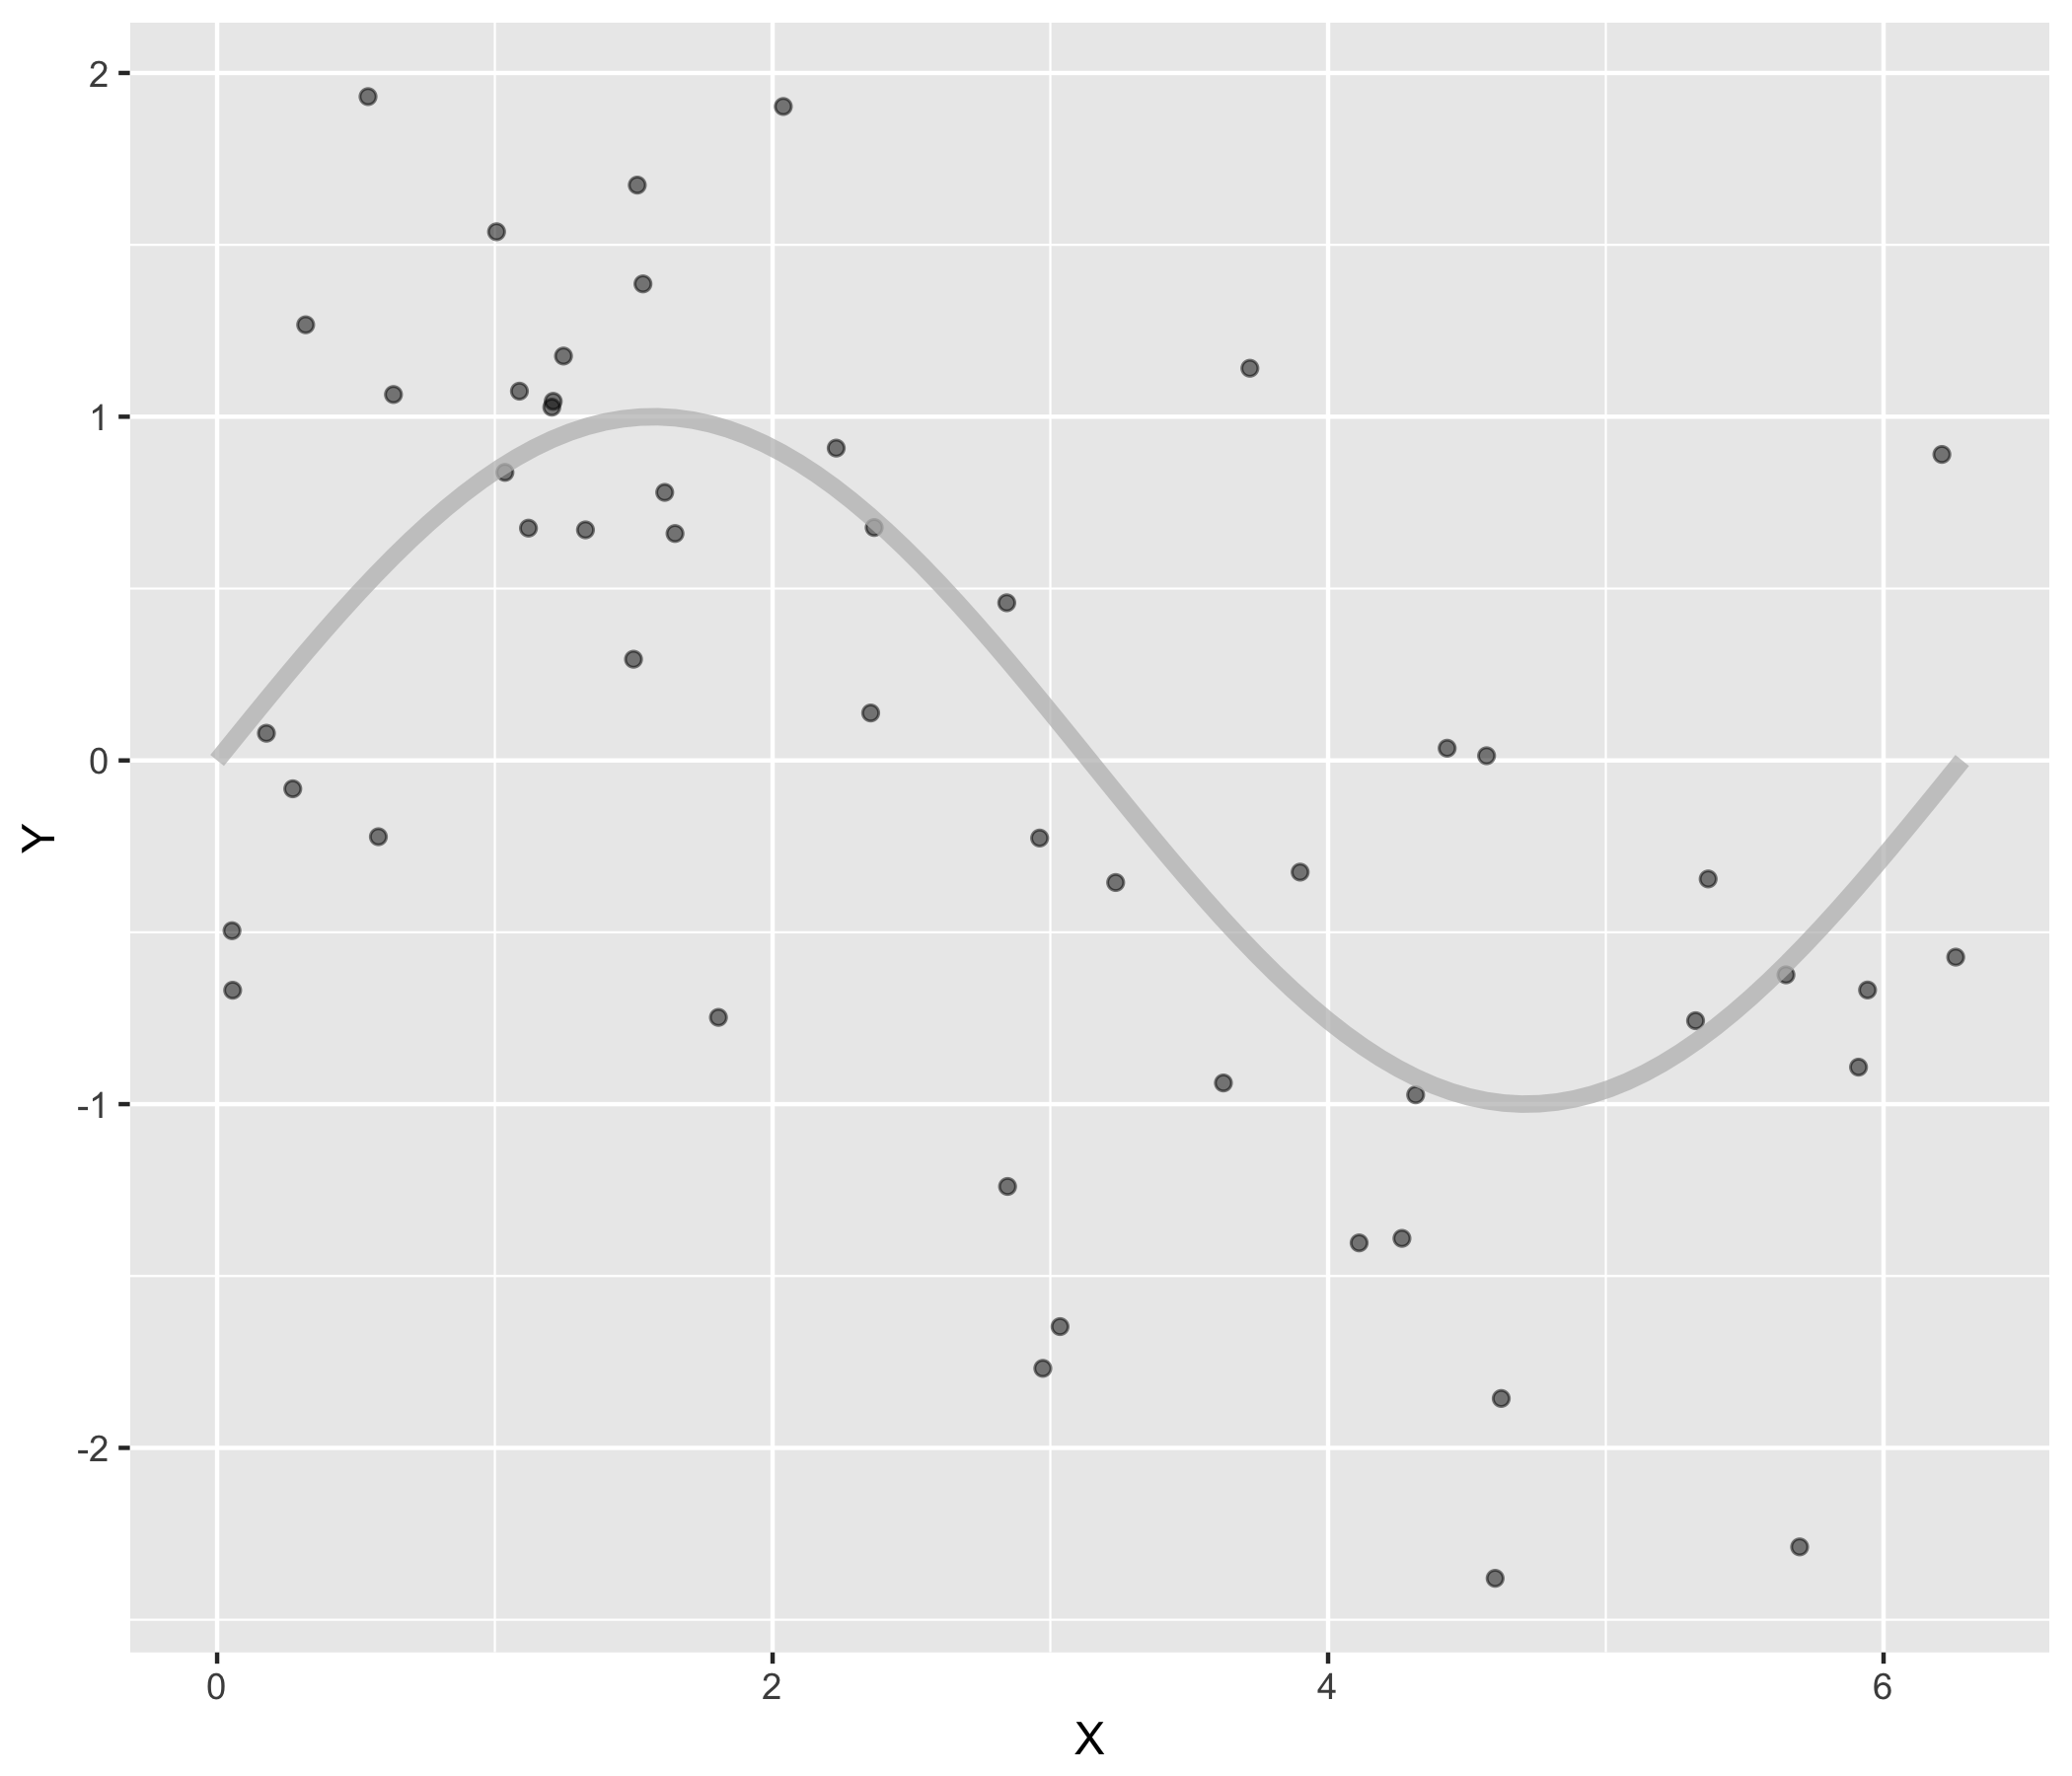
\includegraphics[scale=0.09]{true_signal}
  \end{figure}

  Clearly, the regression function $E(Y \mid X)$ is given by:
  $$ \F(X) = E[ \sin(x) + N(0, \epsilon) \mid x ] = \sin(x) $$
\end{frame}
%
%
\begin{frame}
  The irreducible error component, which does not depend on our choice of
  learning algorithm, is easy to compute straight from the definition:

  \begin{align*}
      \IESE(x) &= E_Y \left[ \left( y - \F(x) \right)^2 \mid x \right] \\
      &= E_Y \left[ \left( \sin(x) + N(0, \epsilon) - \sin(x) \right)^2 \right] \\
      &= E_Y \left[ N(0, \epsilon)^2 \right] \\
      &= \epsilon
  \end{align*}
   
\end{frame}
%
%
\begin{frame}
  We take as our learning algorithm \textbf{linear regression}:
  $$ \LinReg: \D \mapsto \LinReg({\D}_{X}, {\D}_{Y}) $$
  \begin{figure}
    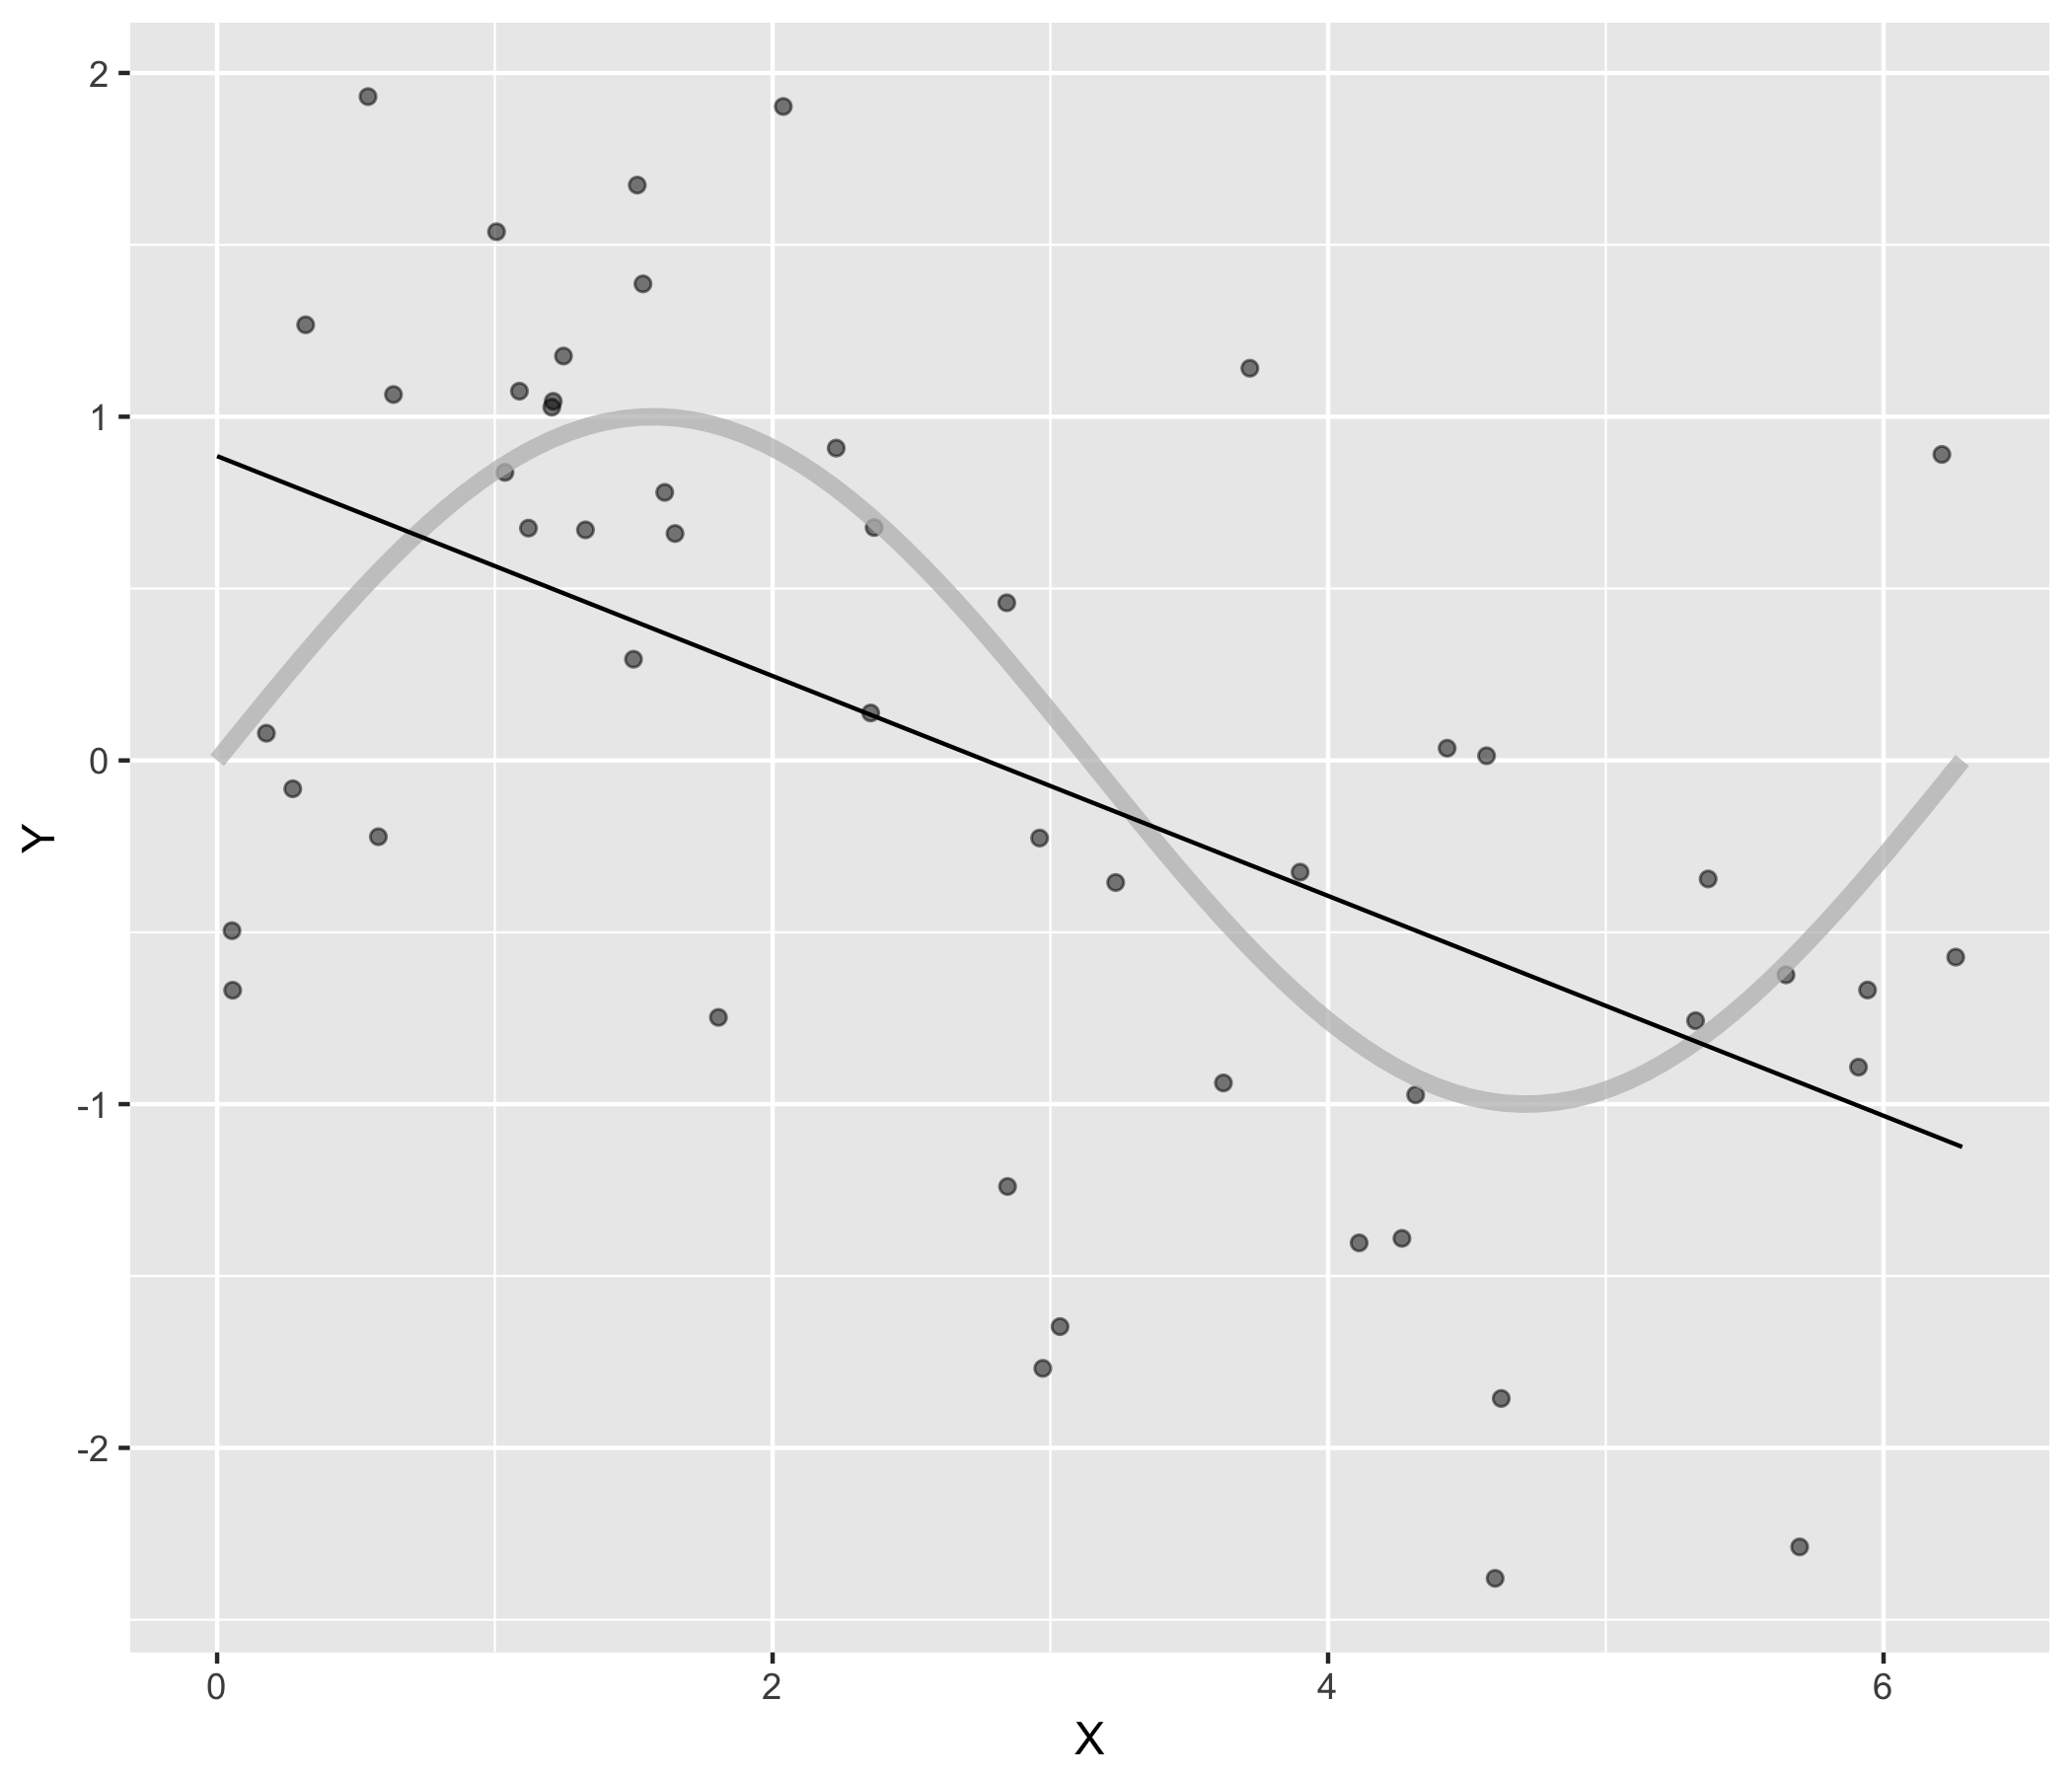
\includegraphics[scale=0.09]{single_fitted_line}
  \end{figure}
\end{frame}
%
%
\begin{frame}
  Let's study the bias of our toy model.  Recall the definition:
  \begin{align*}
    \BIAS (x)^2 = \left( \F(x) - Ef(x) \right)^2
  \end{align*}
  Where:
  \begin{align*}
    Ef(x) = E_D \left[ f(x; \D) \mid x \right] \\ 
  \end{align*}
  is the expected output of our modeling algorithm.
\end{frame}
%
%
\begin{frame}
  For our toy situation we can calculate $Ef$ numerically (I used scipy):
  $$ Ef(x) \approx -0.304 x +  0.955 $$
\end{frame}
%
%
\begin{frame}
  \begin{figure}
    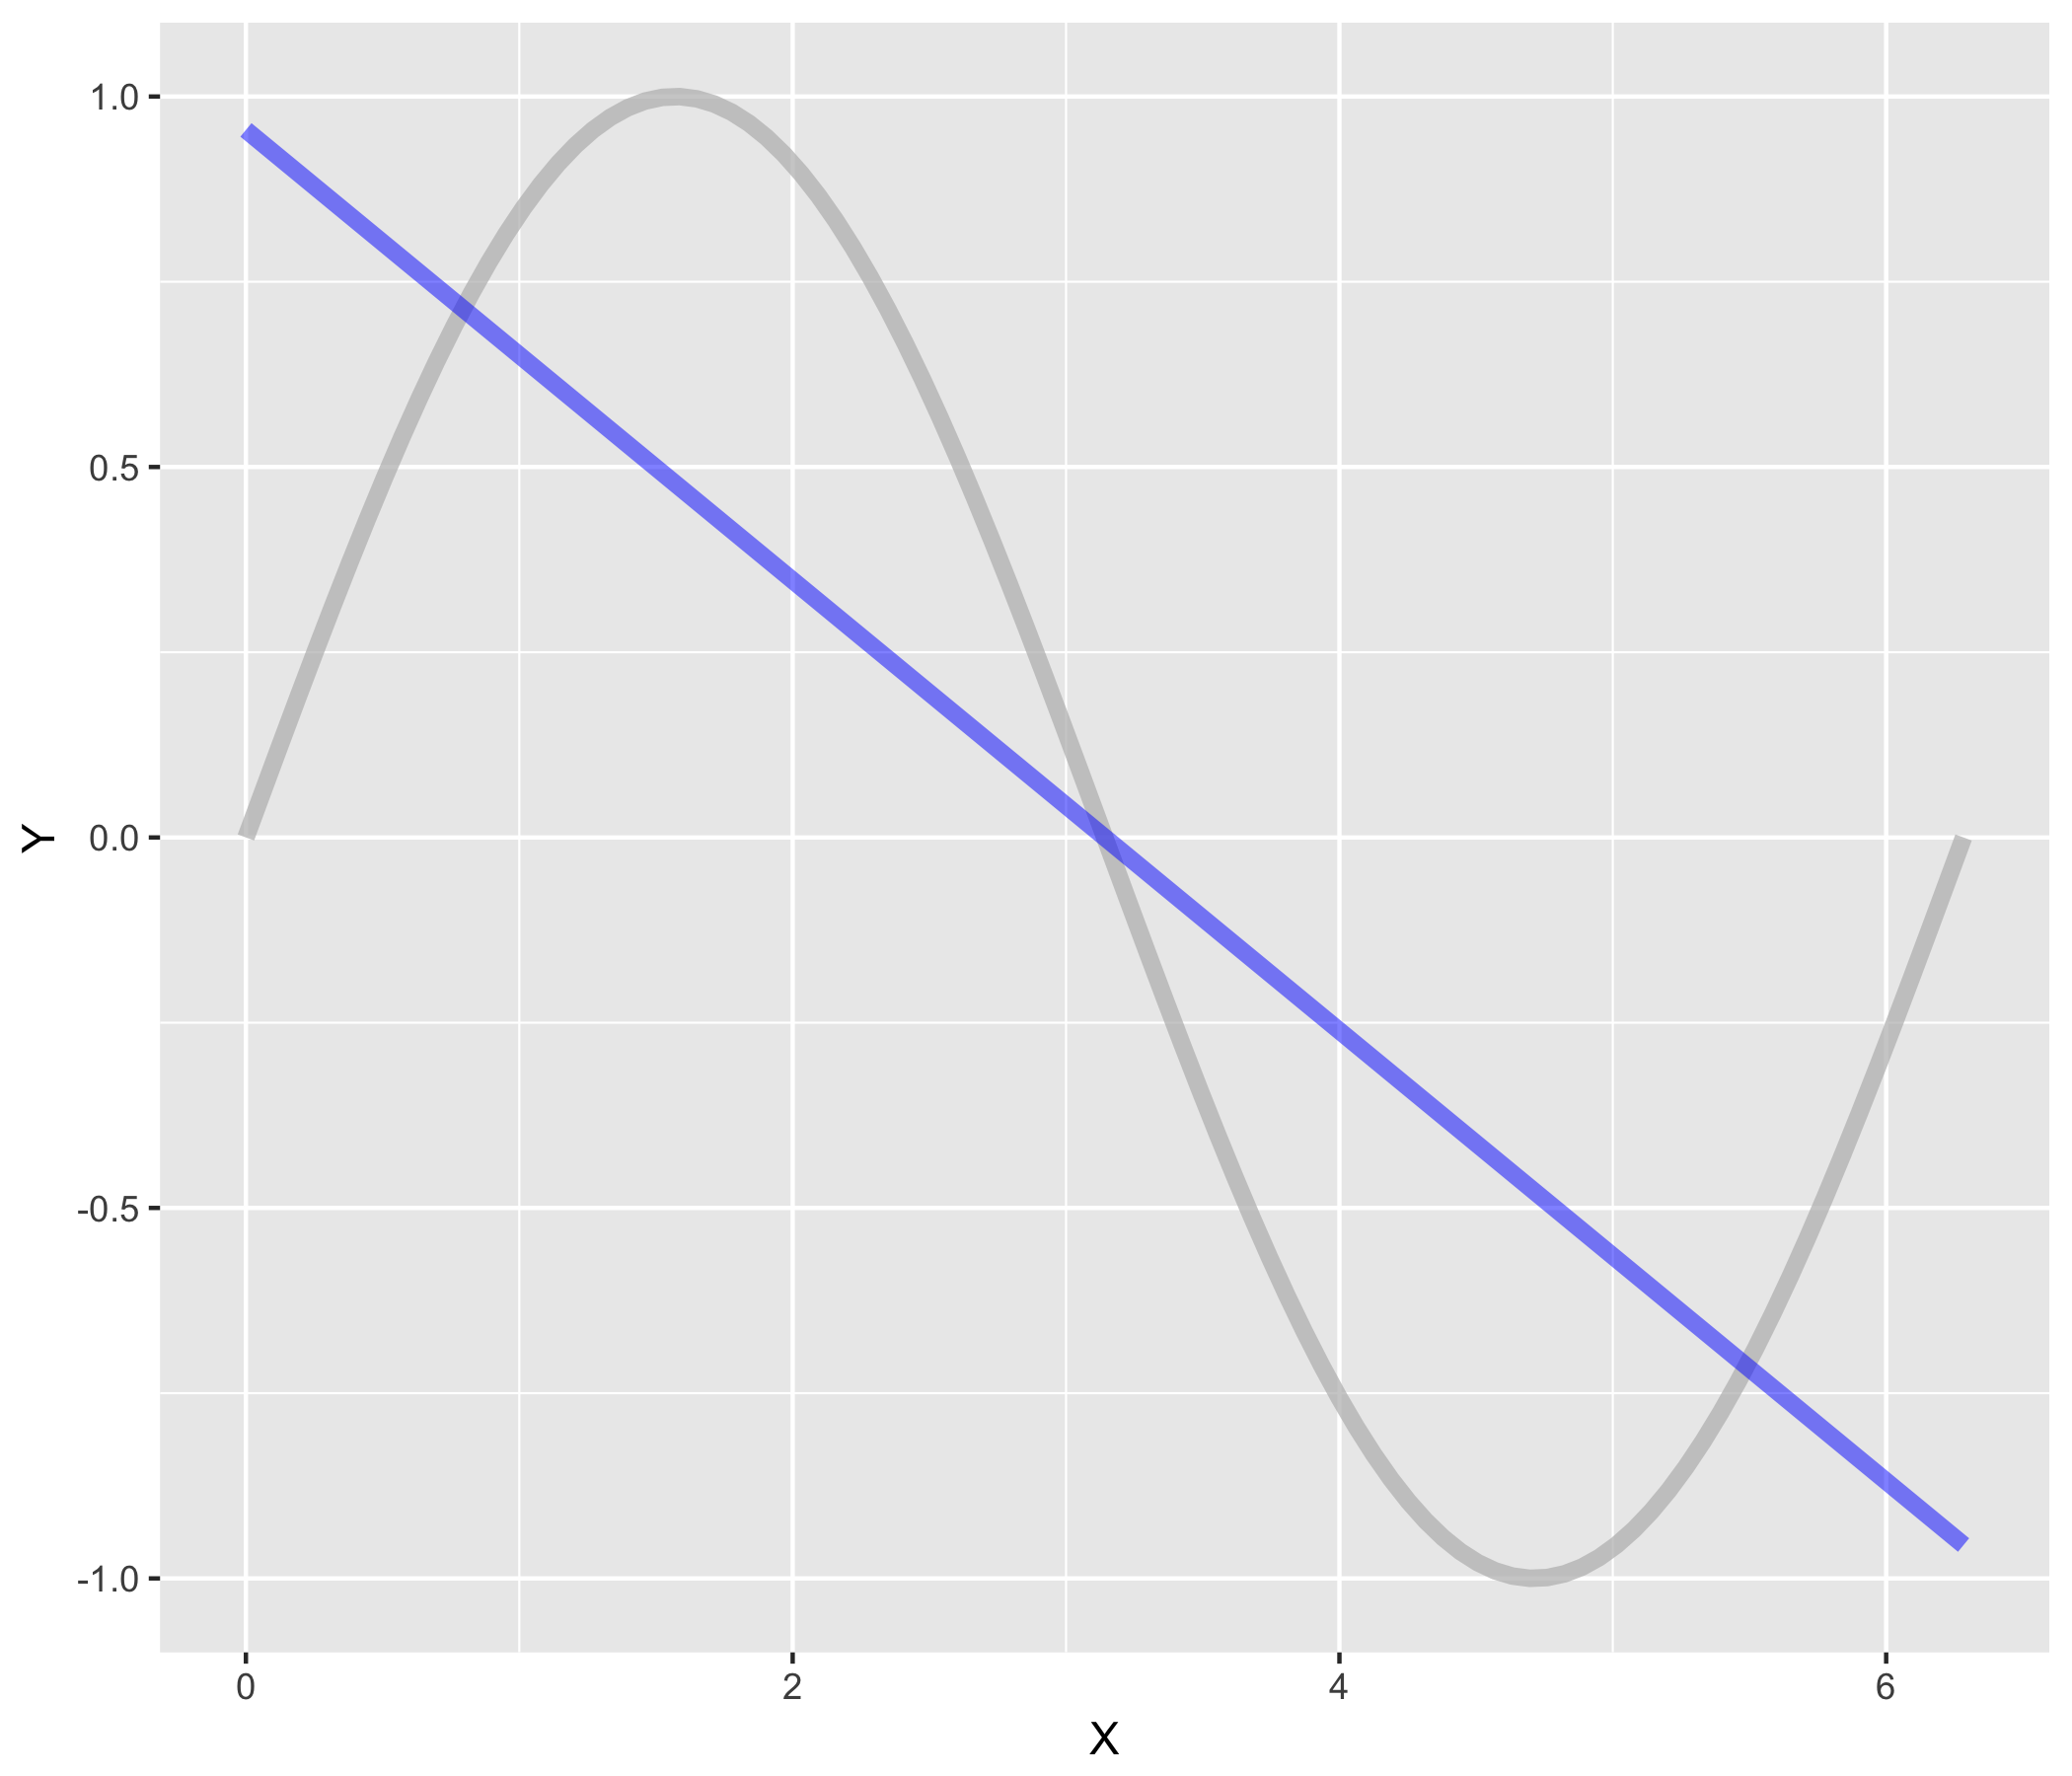
\includegraphics[scale=0.12]{best_linear_fit}
  \end{figure}
\end{frame}
%
%
\begin{frame}
  The bias at a point is the square of the vertical distance between the true
  signal and the best linear fit.
  \begin{figure}
    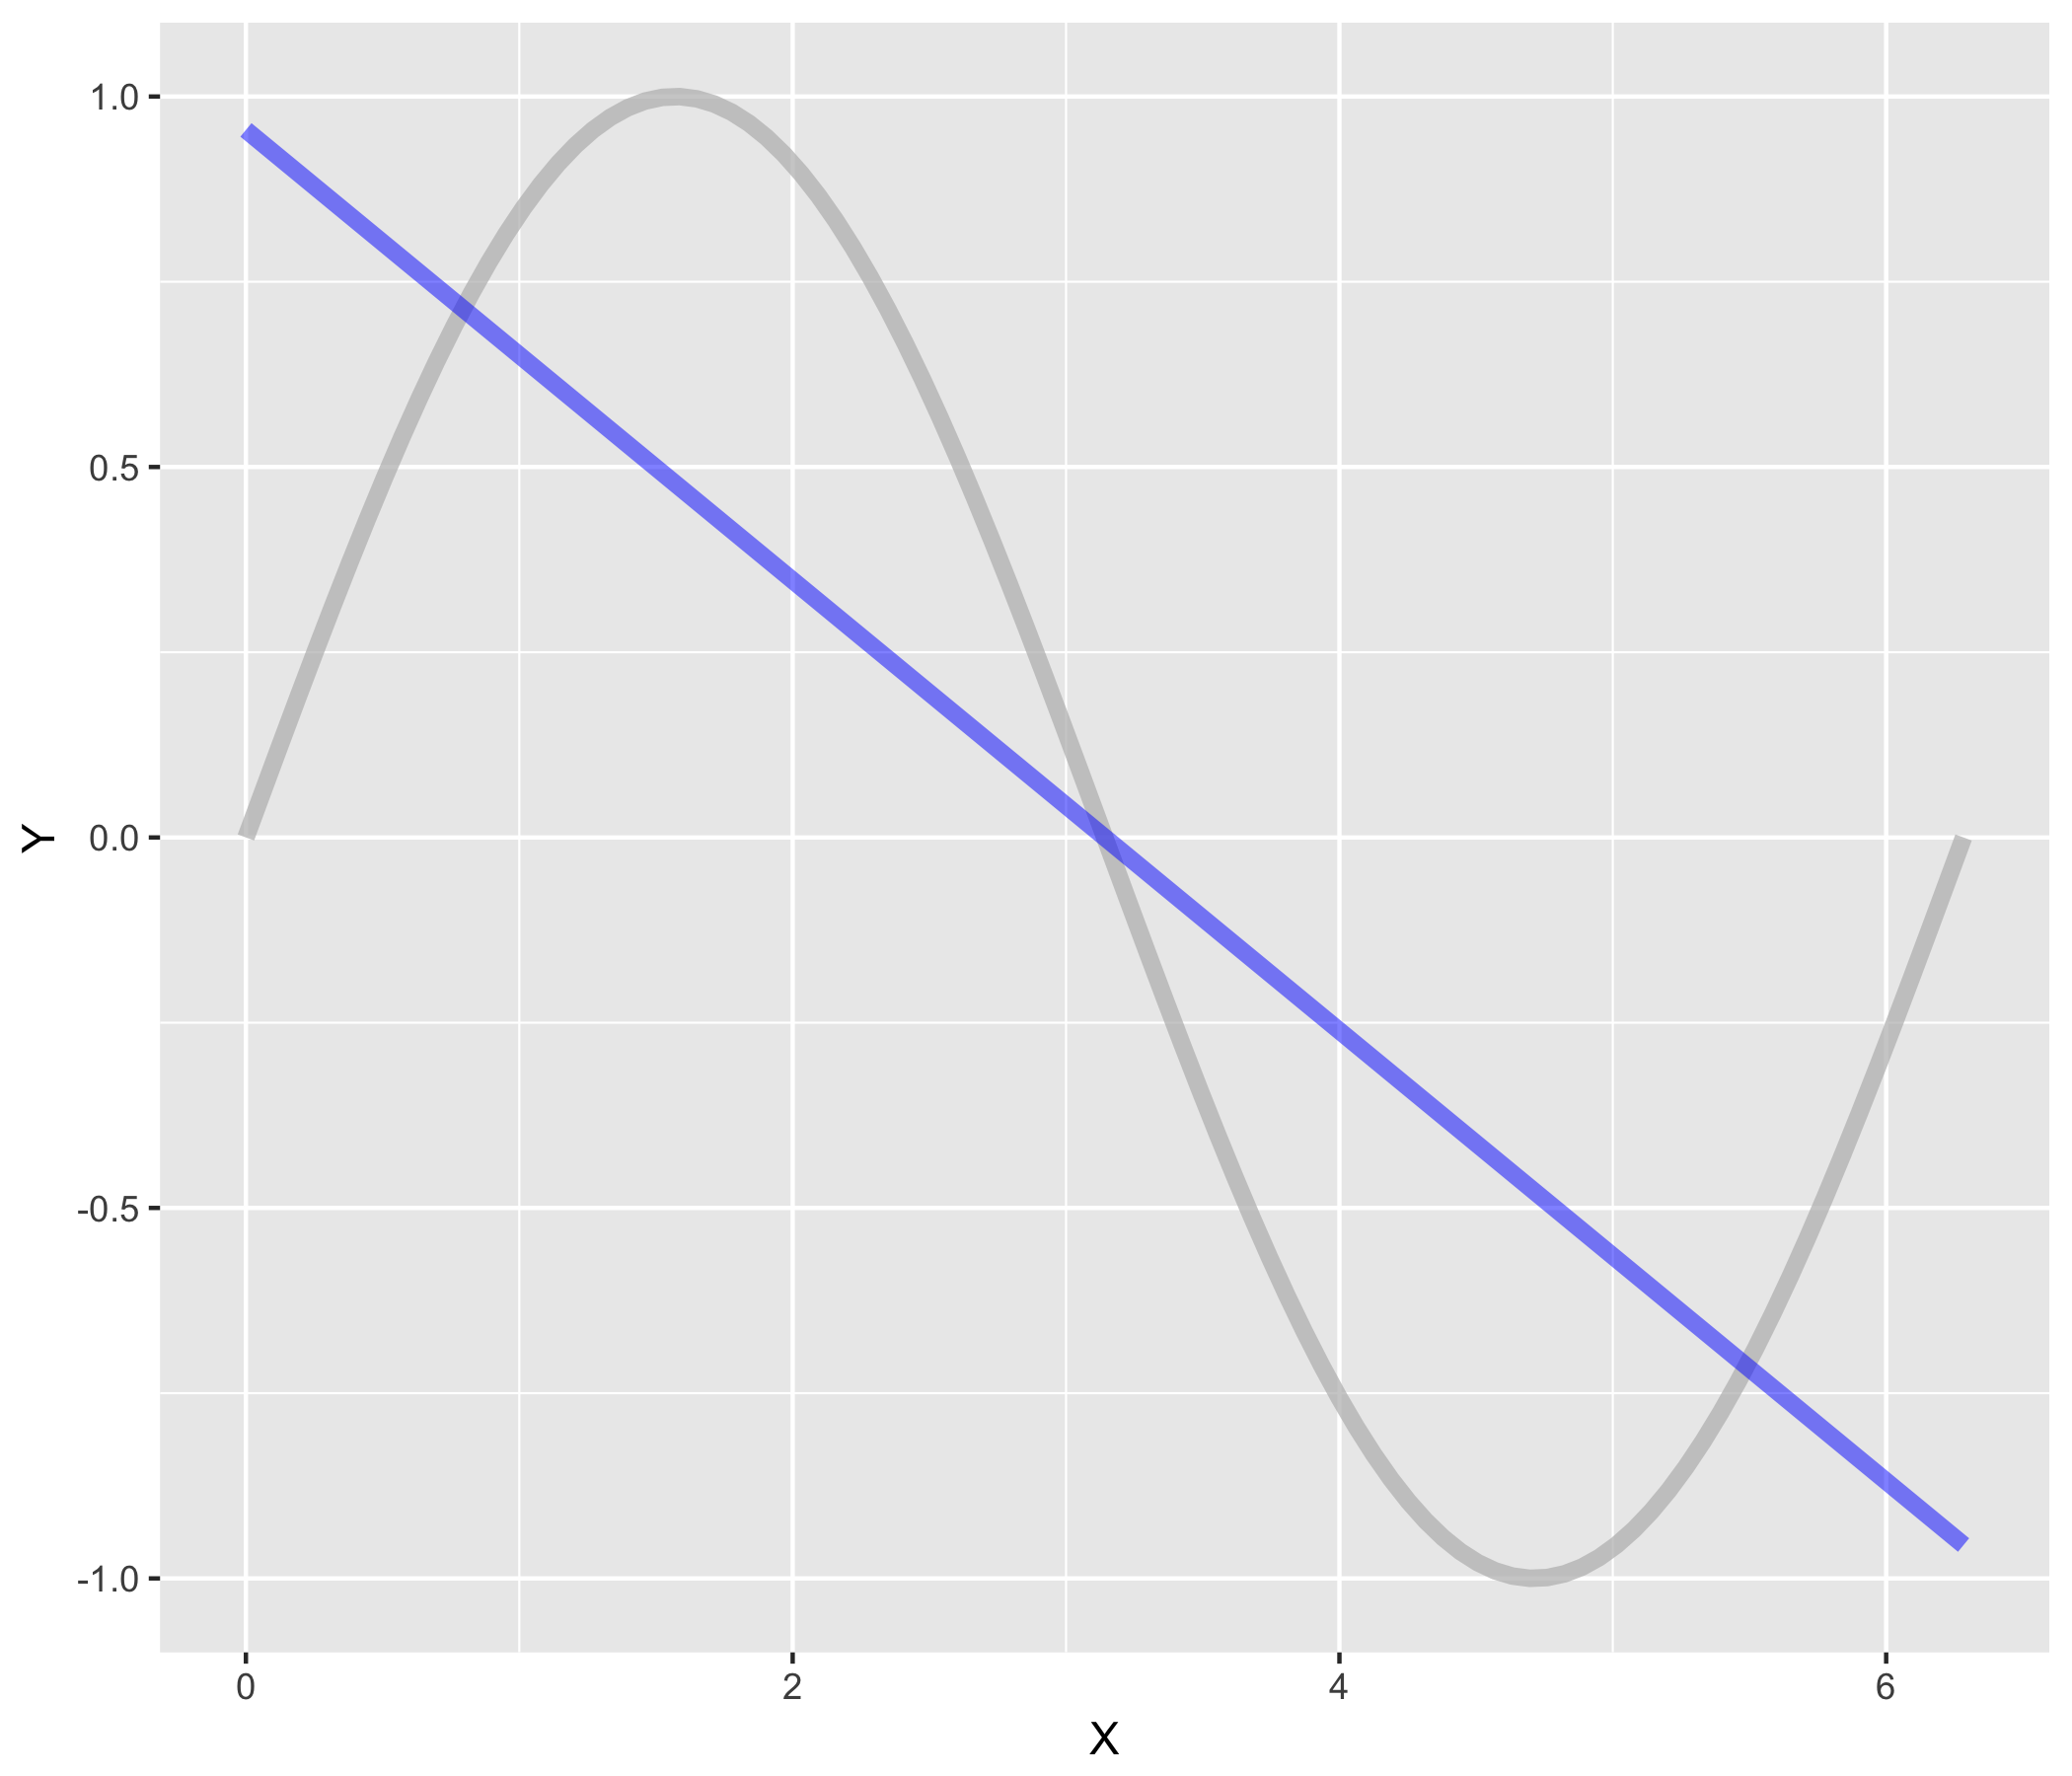
\includegraphics[scale=0.08]{best_linear_fit}
  \end{figure}
\end{frame}
%
%
\begin{frame}
  The total bias is the expectation of the pointwise bias.  Visually, we can
  think of the unsigned area between the best linear fit and the true signal:
  \begin{figure}
    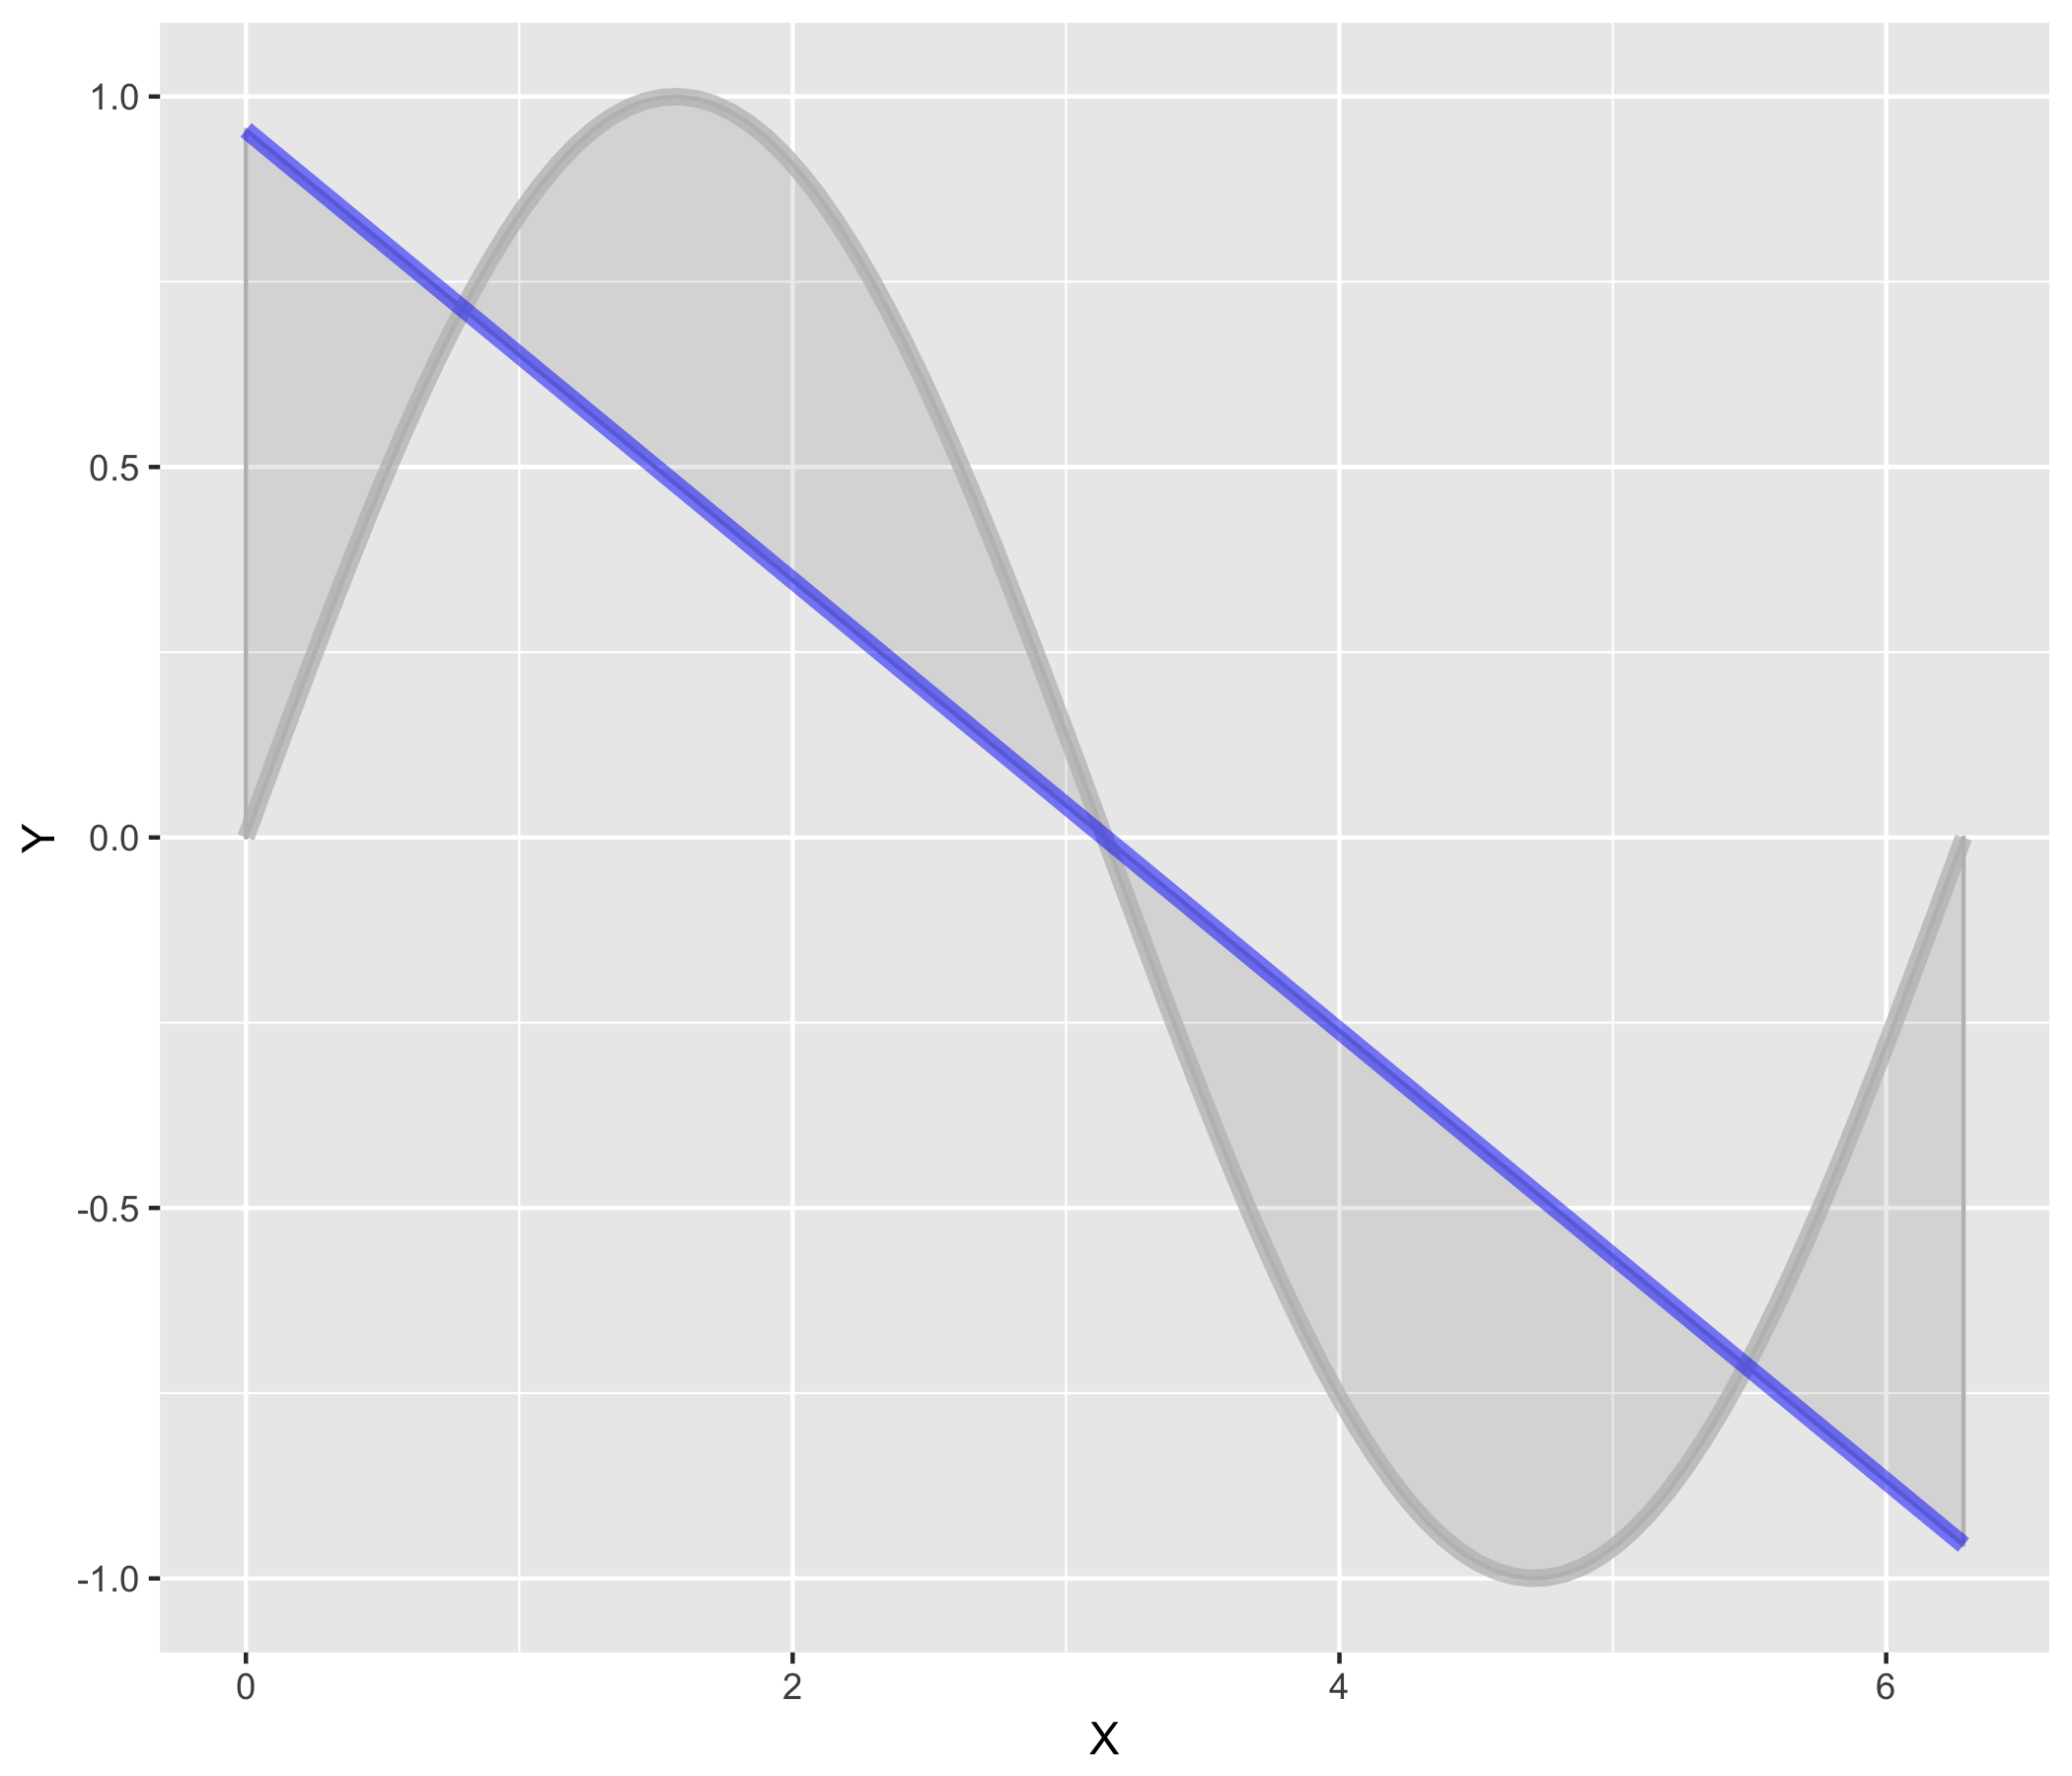
\includegraphics[scale=0.08]{model_bias}
  \end{figure}
\end{frame}
%
%
\begin{frame}
  The total bias can be explicitly calculated in this case (I used a numerical
  integration routine):
  $$ {\BIAS}^2 = E_X \left[ \left( \F(x) - Ef(x) \right)^2 \right] \approx 1.23
  $$
\end{frame}
%
%
\begin{frame}
  Bias can be lowered by making our learning algorithm more complex.  For
  example, fitting a \textit{cubic} regression lowers the bias of our model
  considerably:
  \begin{figure}
    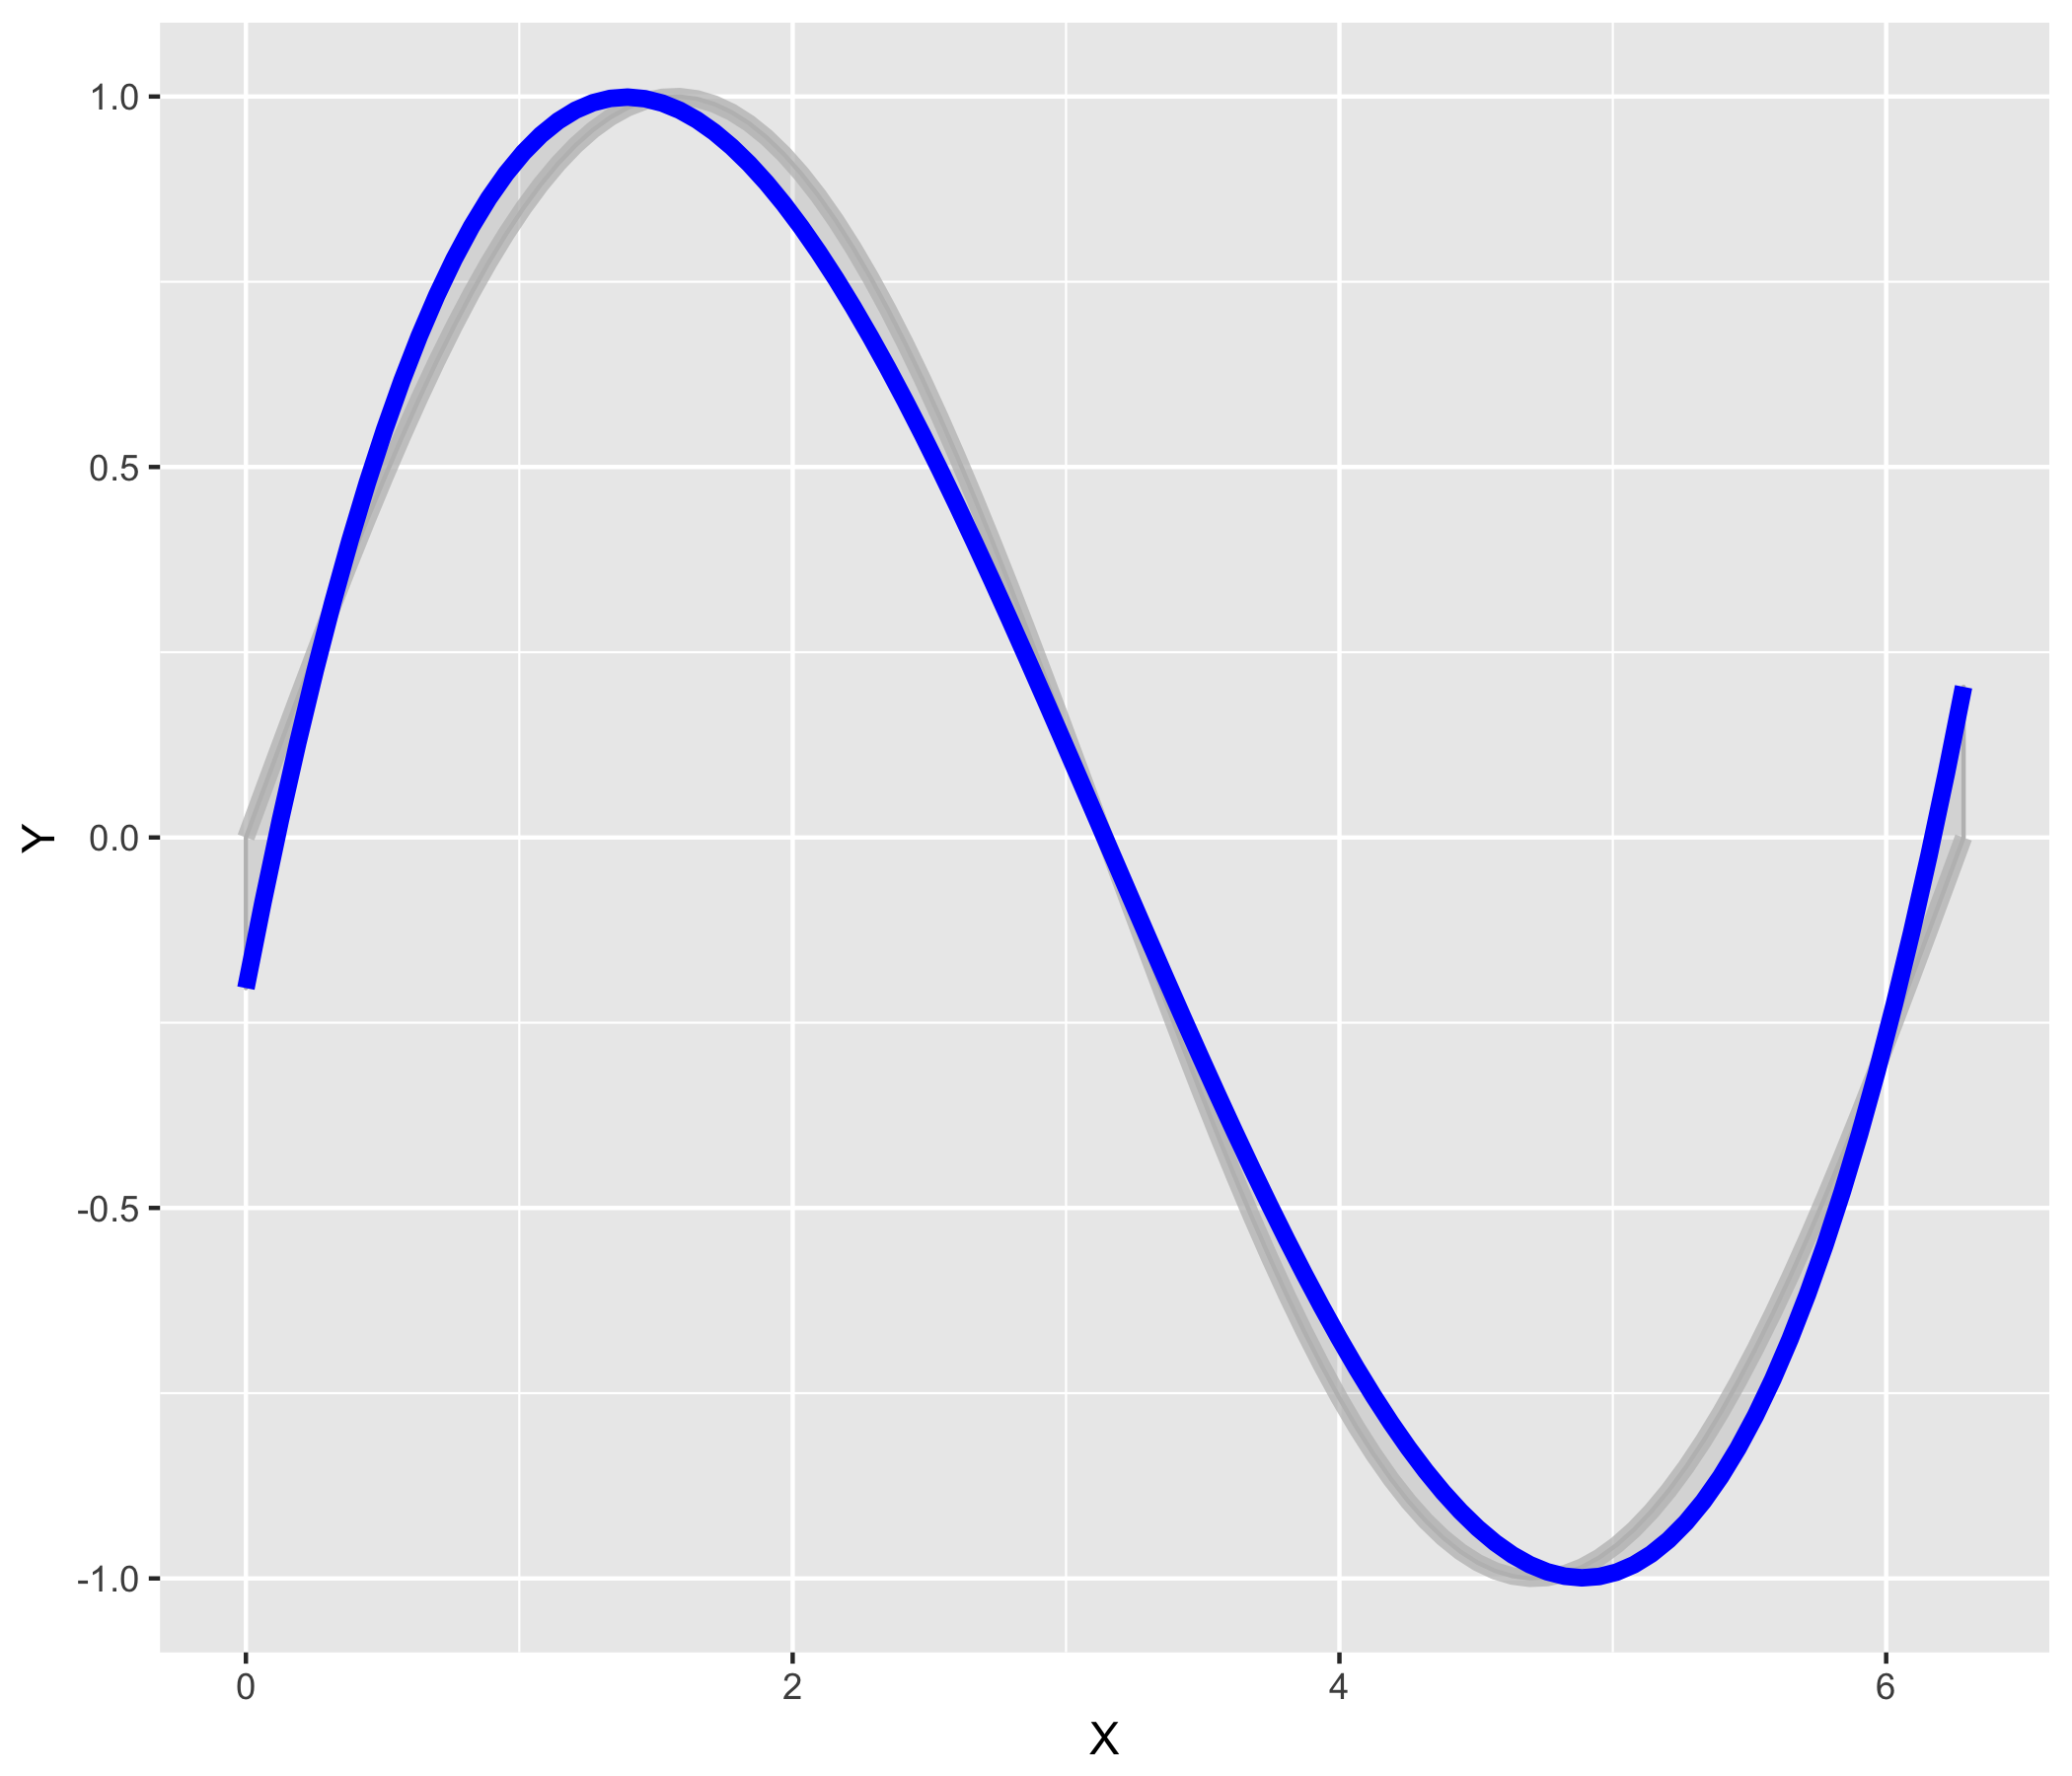
\includegraphics[scale=0.08]{cubic_model_bias}
  \end{figure}
  $$ {\BIAS}^2 = E_X \left[ \left( \F(x) - Ef(x) \right)^2 \right] \approx 0.028
  $$
\end{frame}
%
%
\begin{frame}
  It is tempting to want to lower the bias as much as possible, as this brings
  our expected model close to reality, unfortunately, the model variance is a
  price we pay.
\end{frame}
%
%
\begin{frame}
  The model variance measures how sensitive our estimate is to the specific
  training data used:
      $$ E_{\D} \left[ \left( Ef(x) - f(x,\D) \right)^2 \mid x \right] $$
\end{frame}
%
%
\begin{frame}
   Lines fit to different data sampled from our model distribution tend to
   cluster around the best linear fit, but there is a fair amount of variance in
   the clustering:
  \begin{figure}
    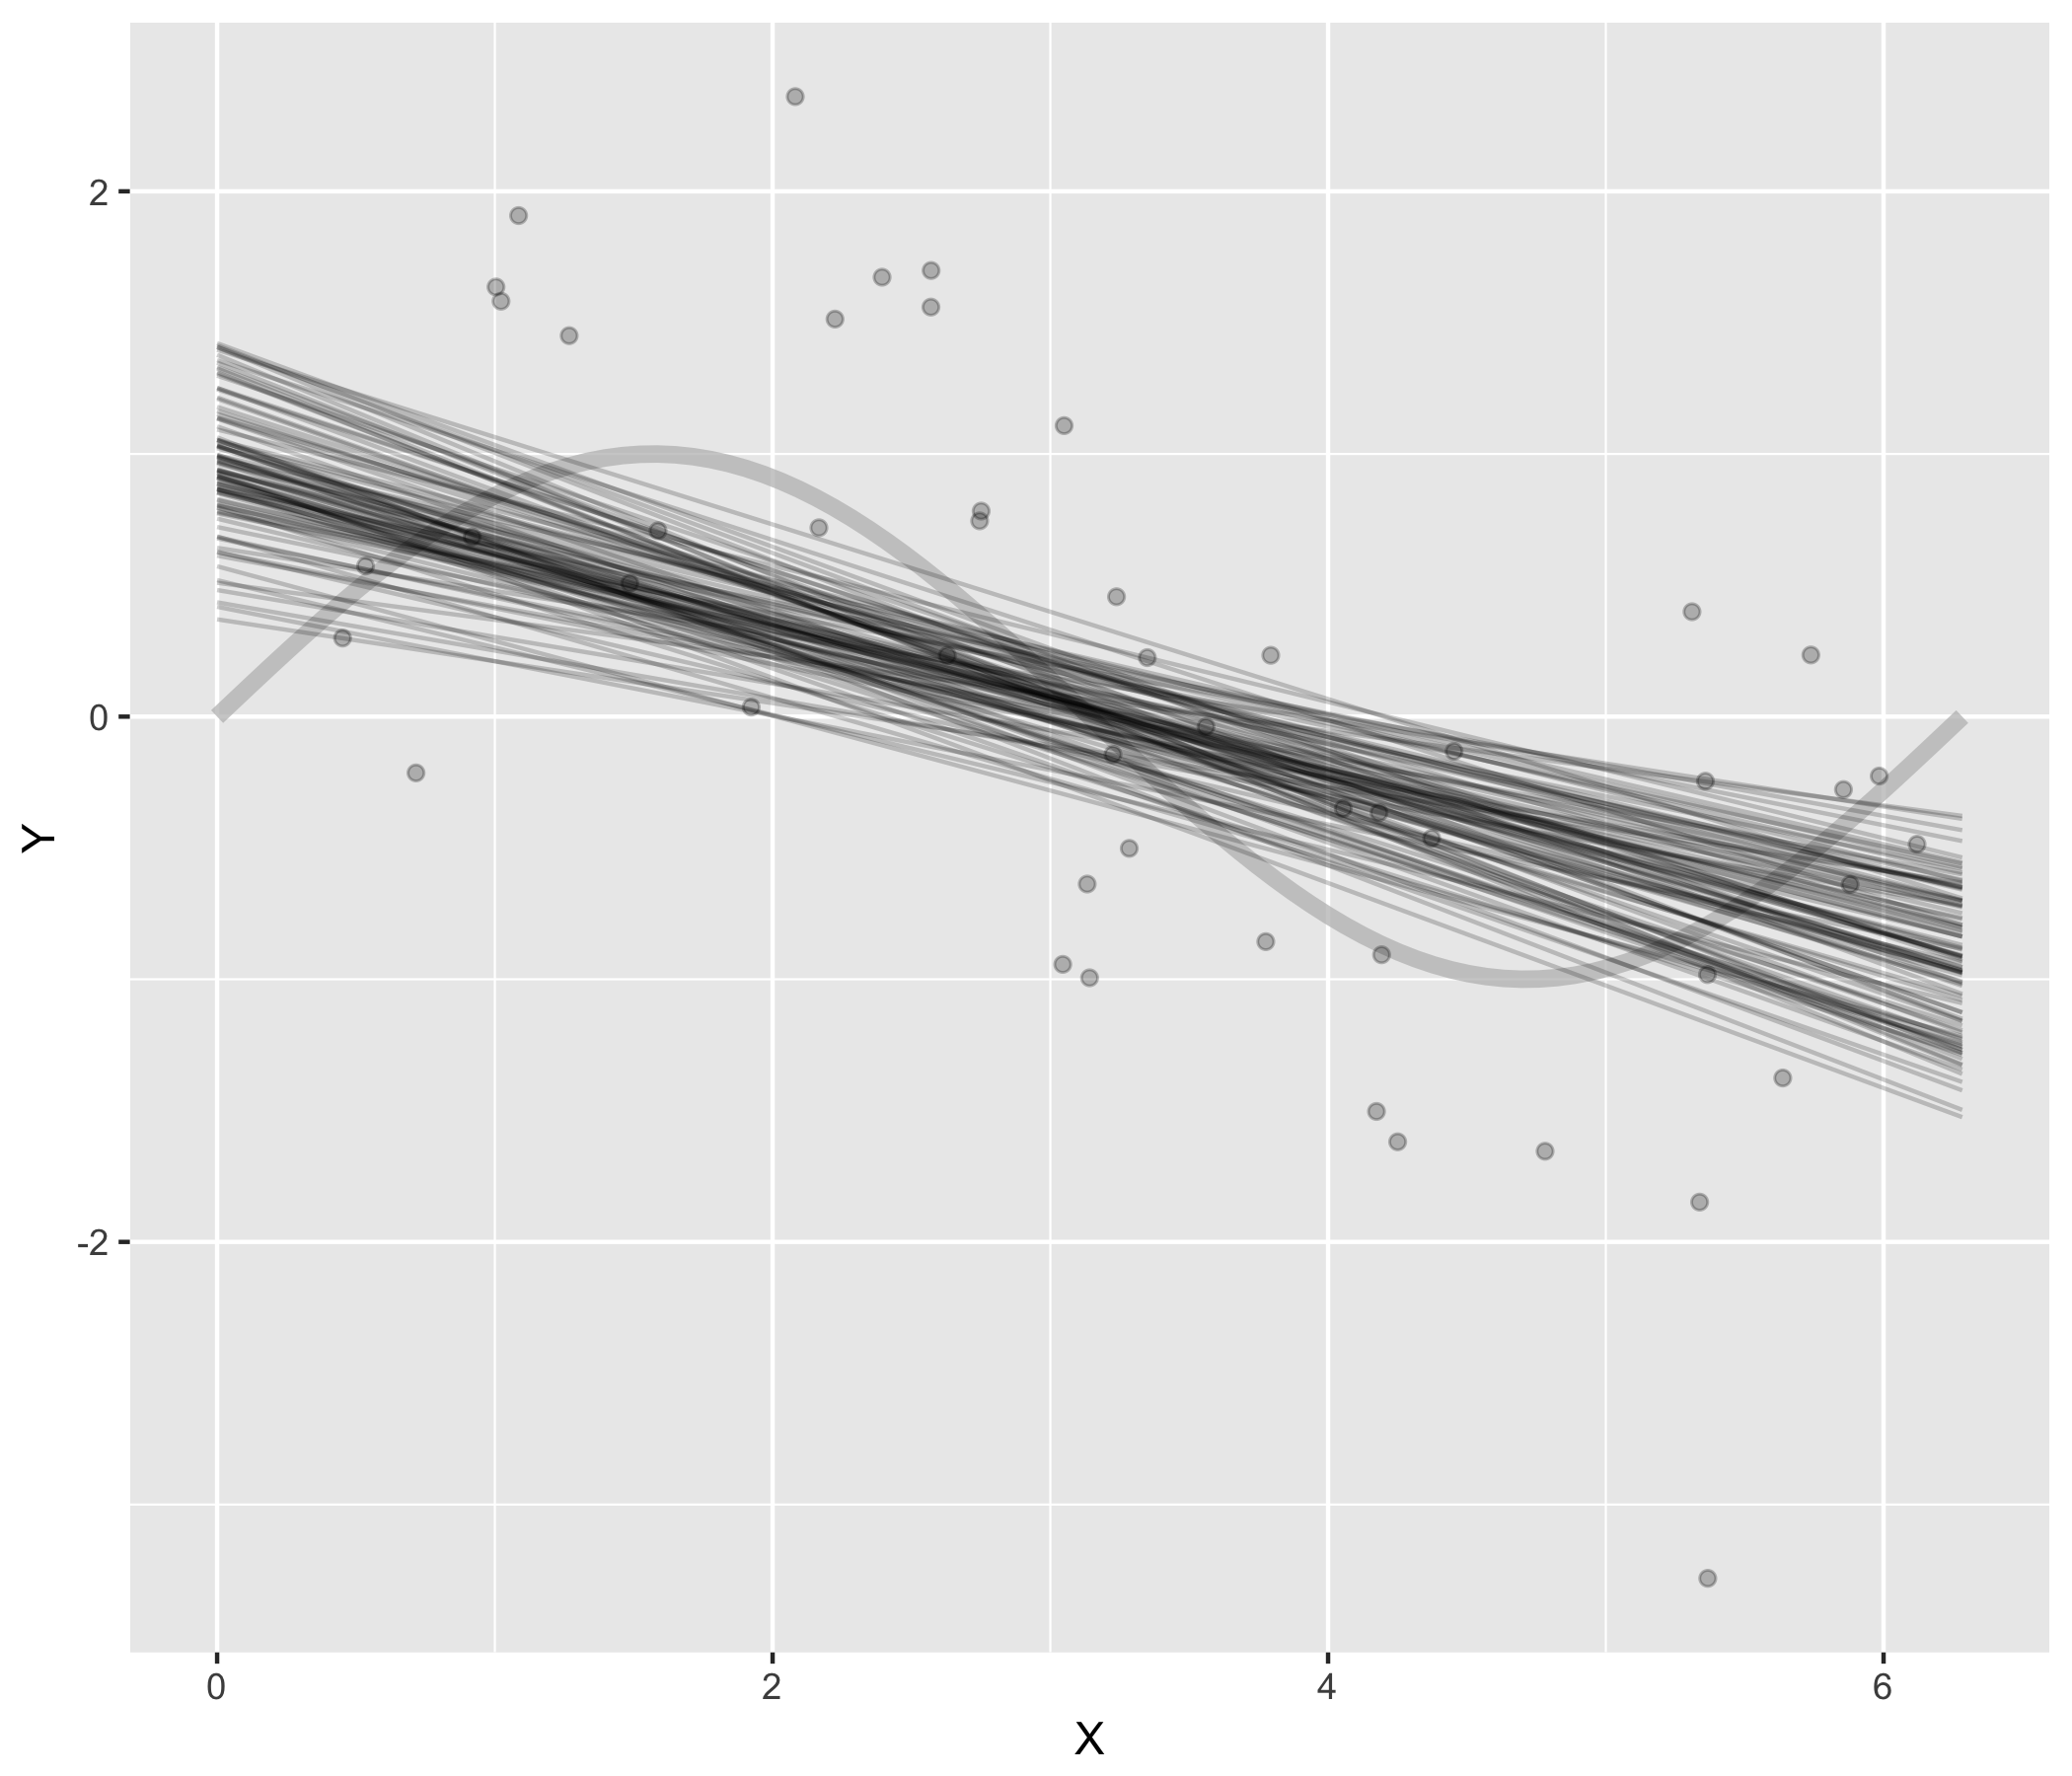
\includegraphics[scale=0.09]{model_variance_standard_samples}
  \end{figure}
\end{frame}
%
%
\begin{frame}
  Increasing the amount of data used to fit reduces the variance:
  \begin{figure}
    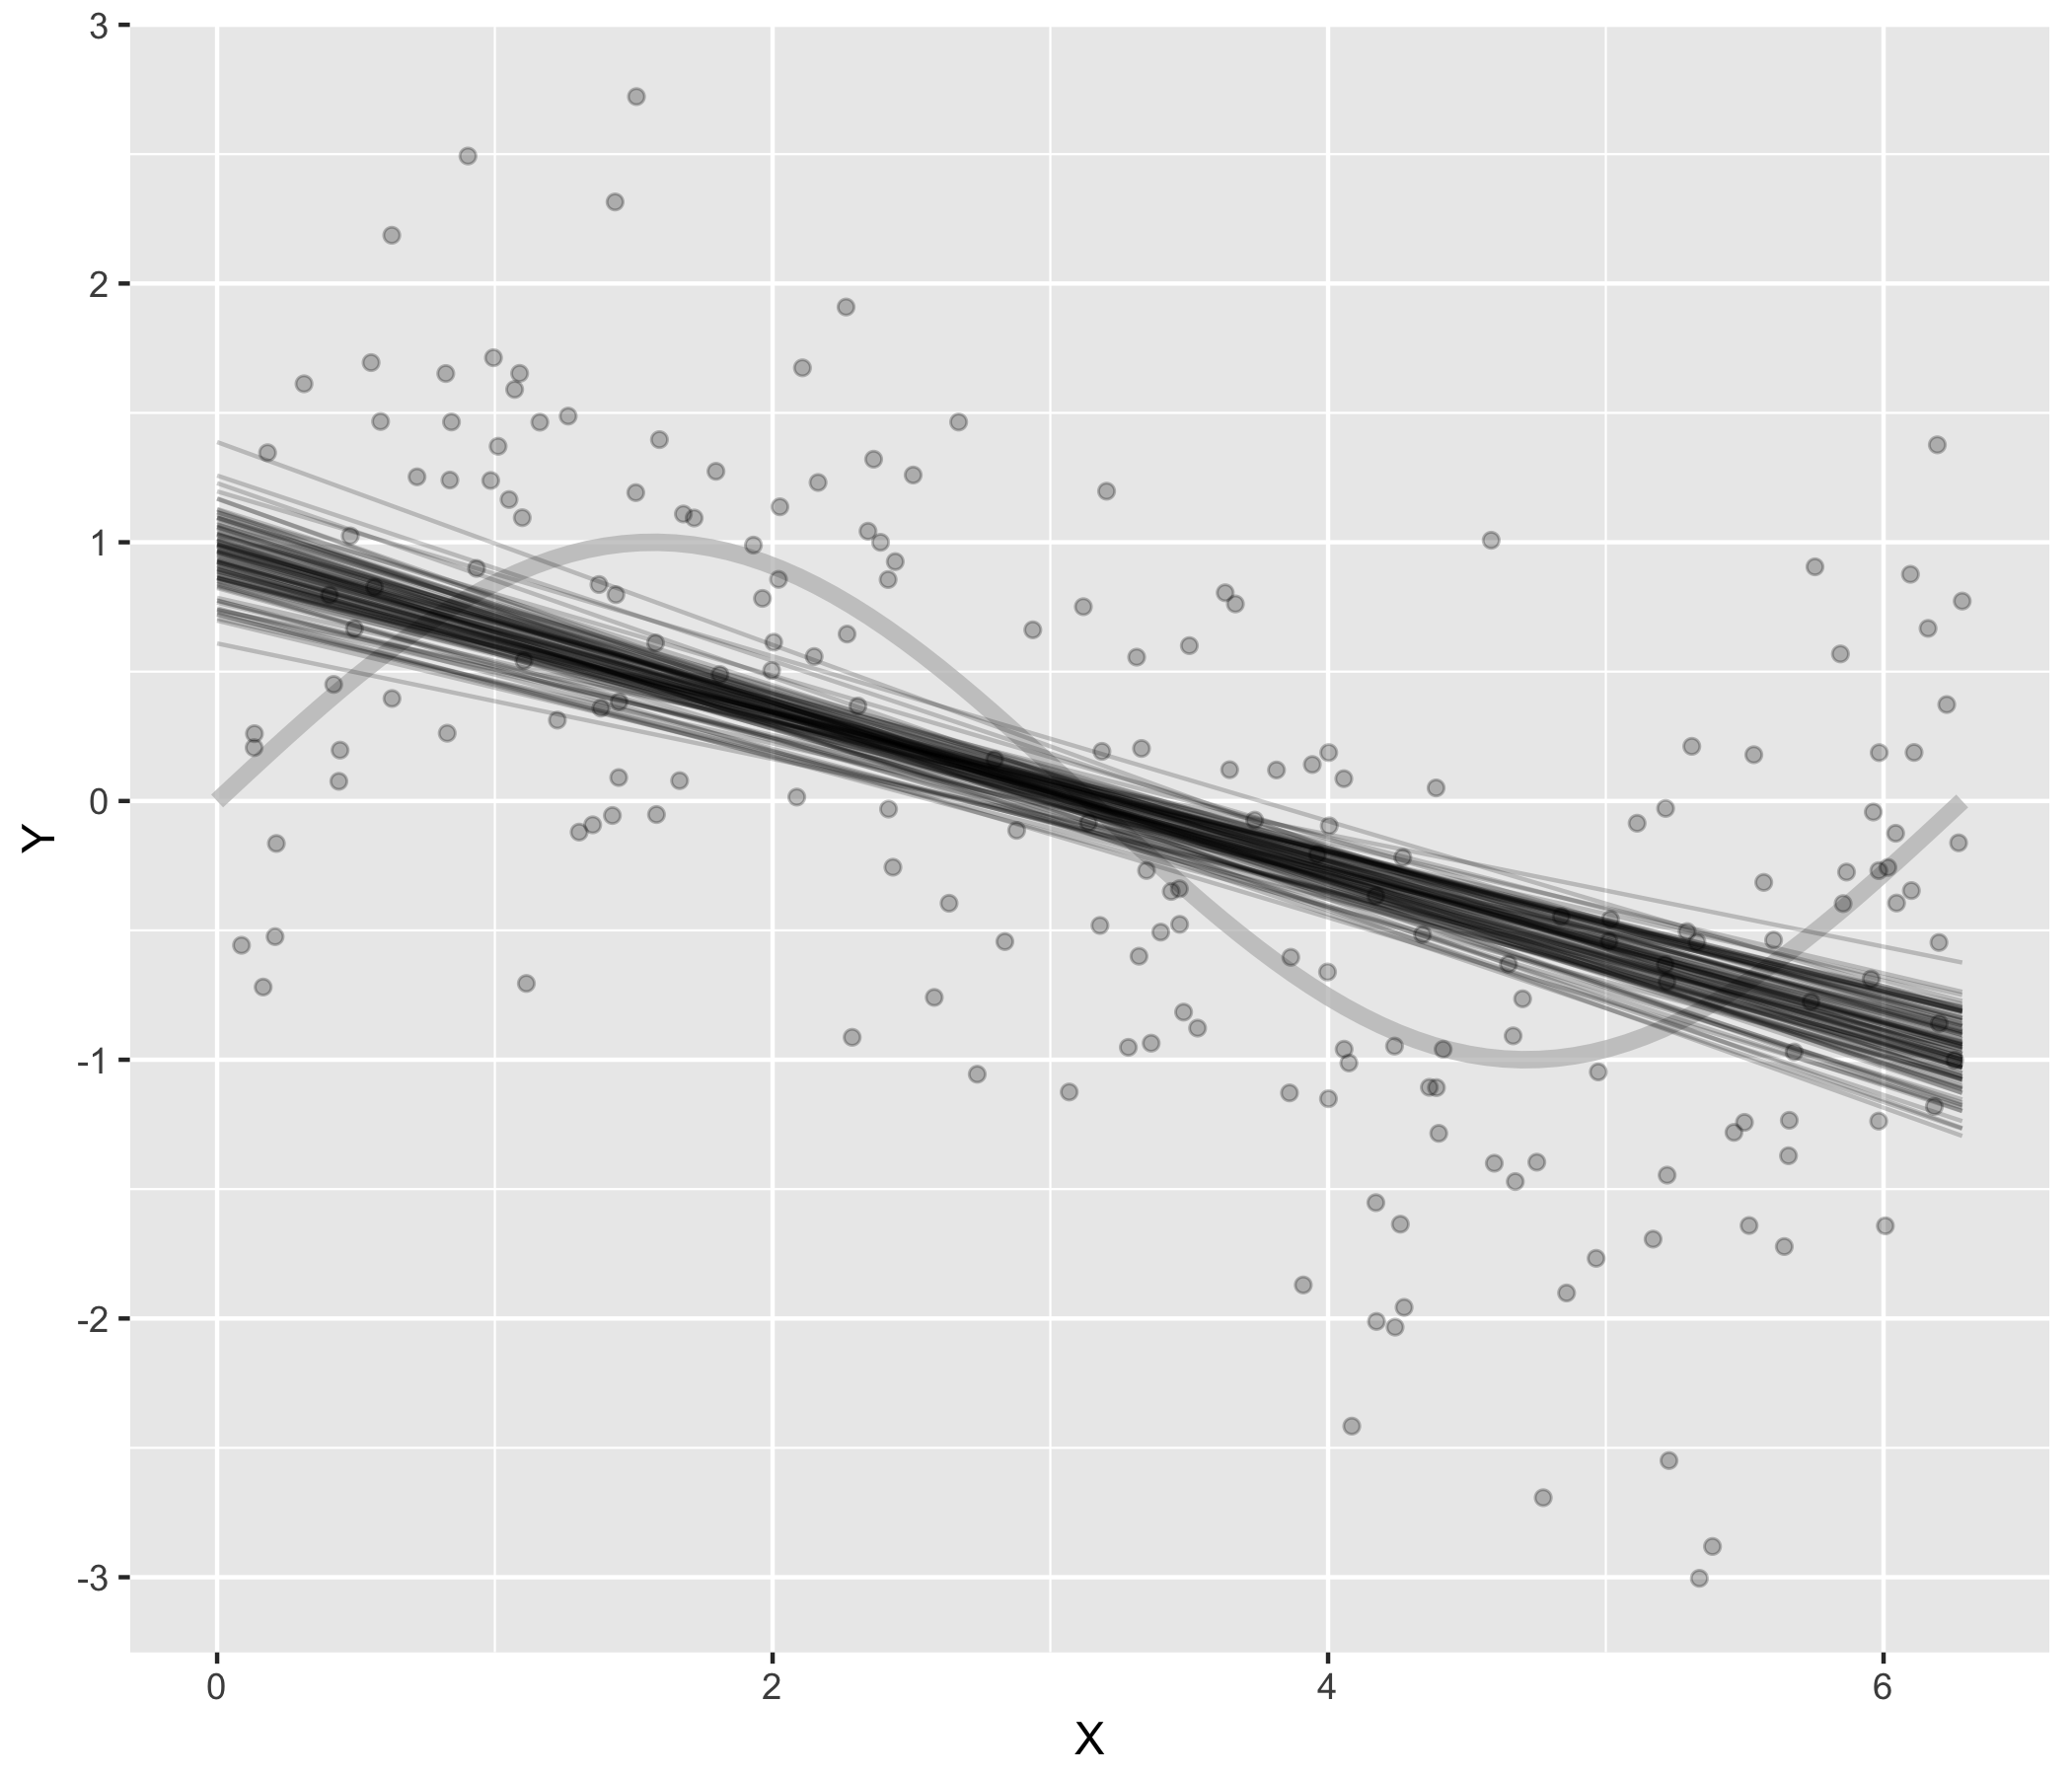
\includegraphics[scale=0.09]{model_variance_more_samples}
  \end{figure}
\end{frame}
%
%
\begin{frame}
  Decreasing the amount of data used to fit increases the variance:
  \begin{figure}
    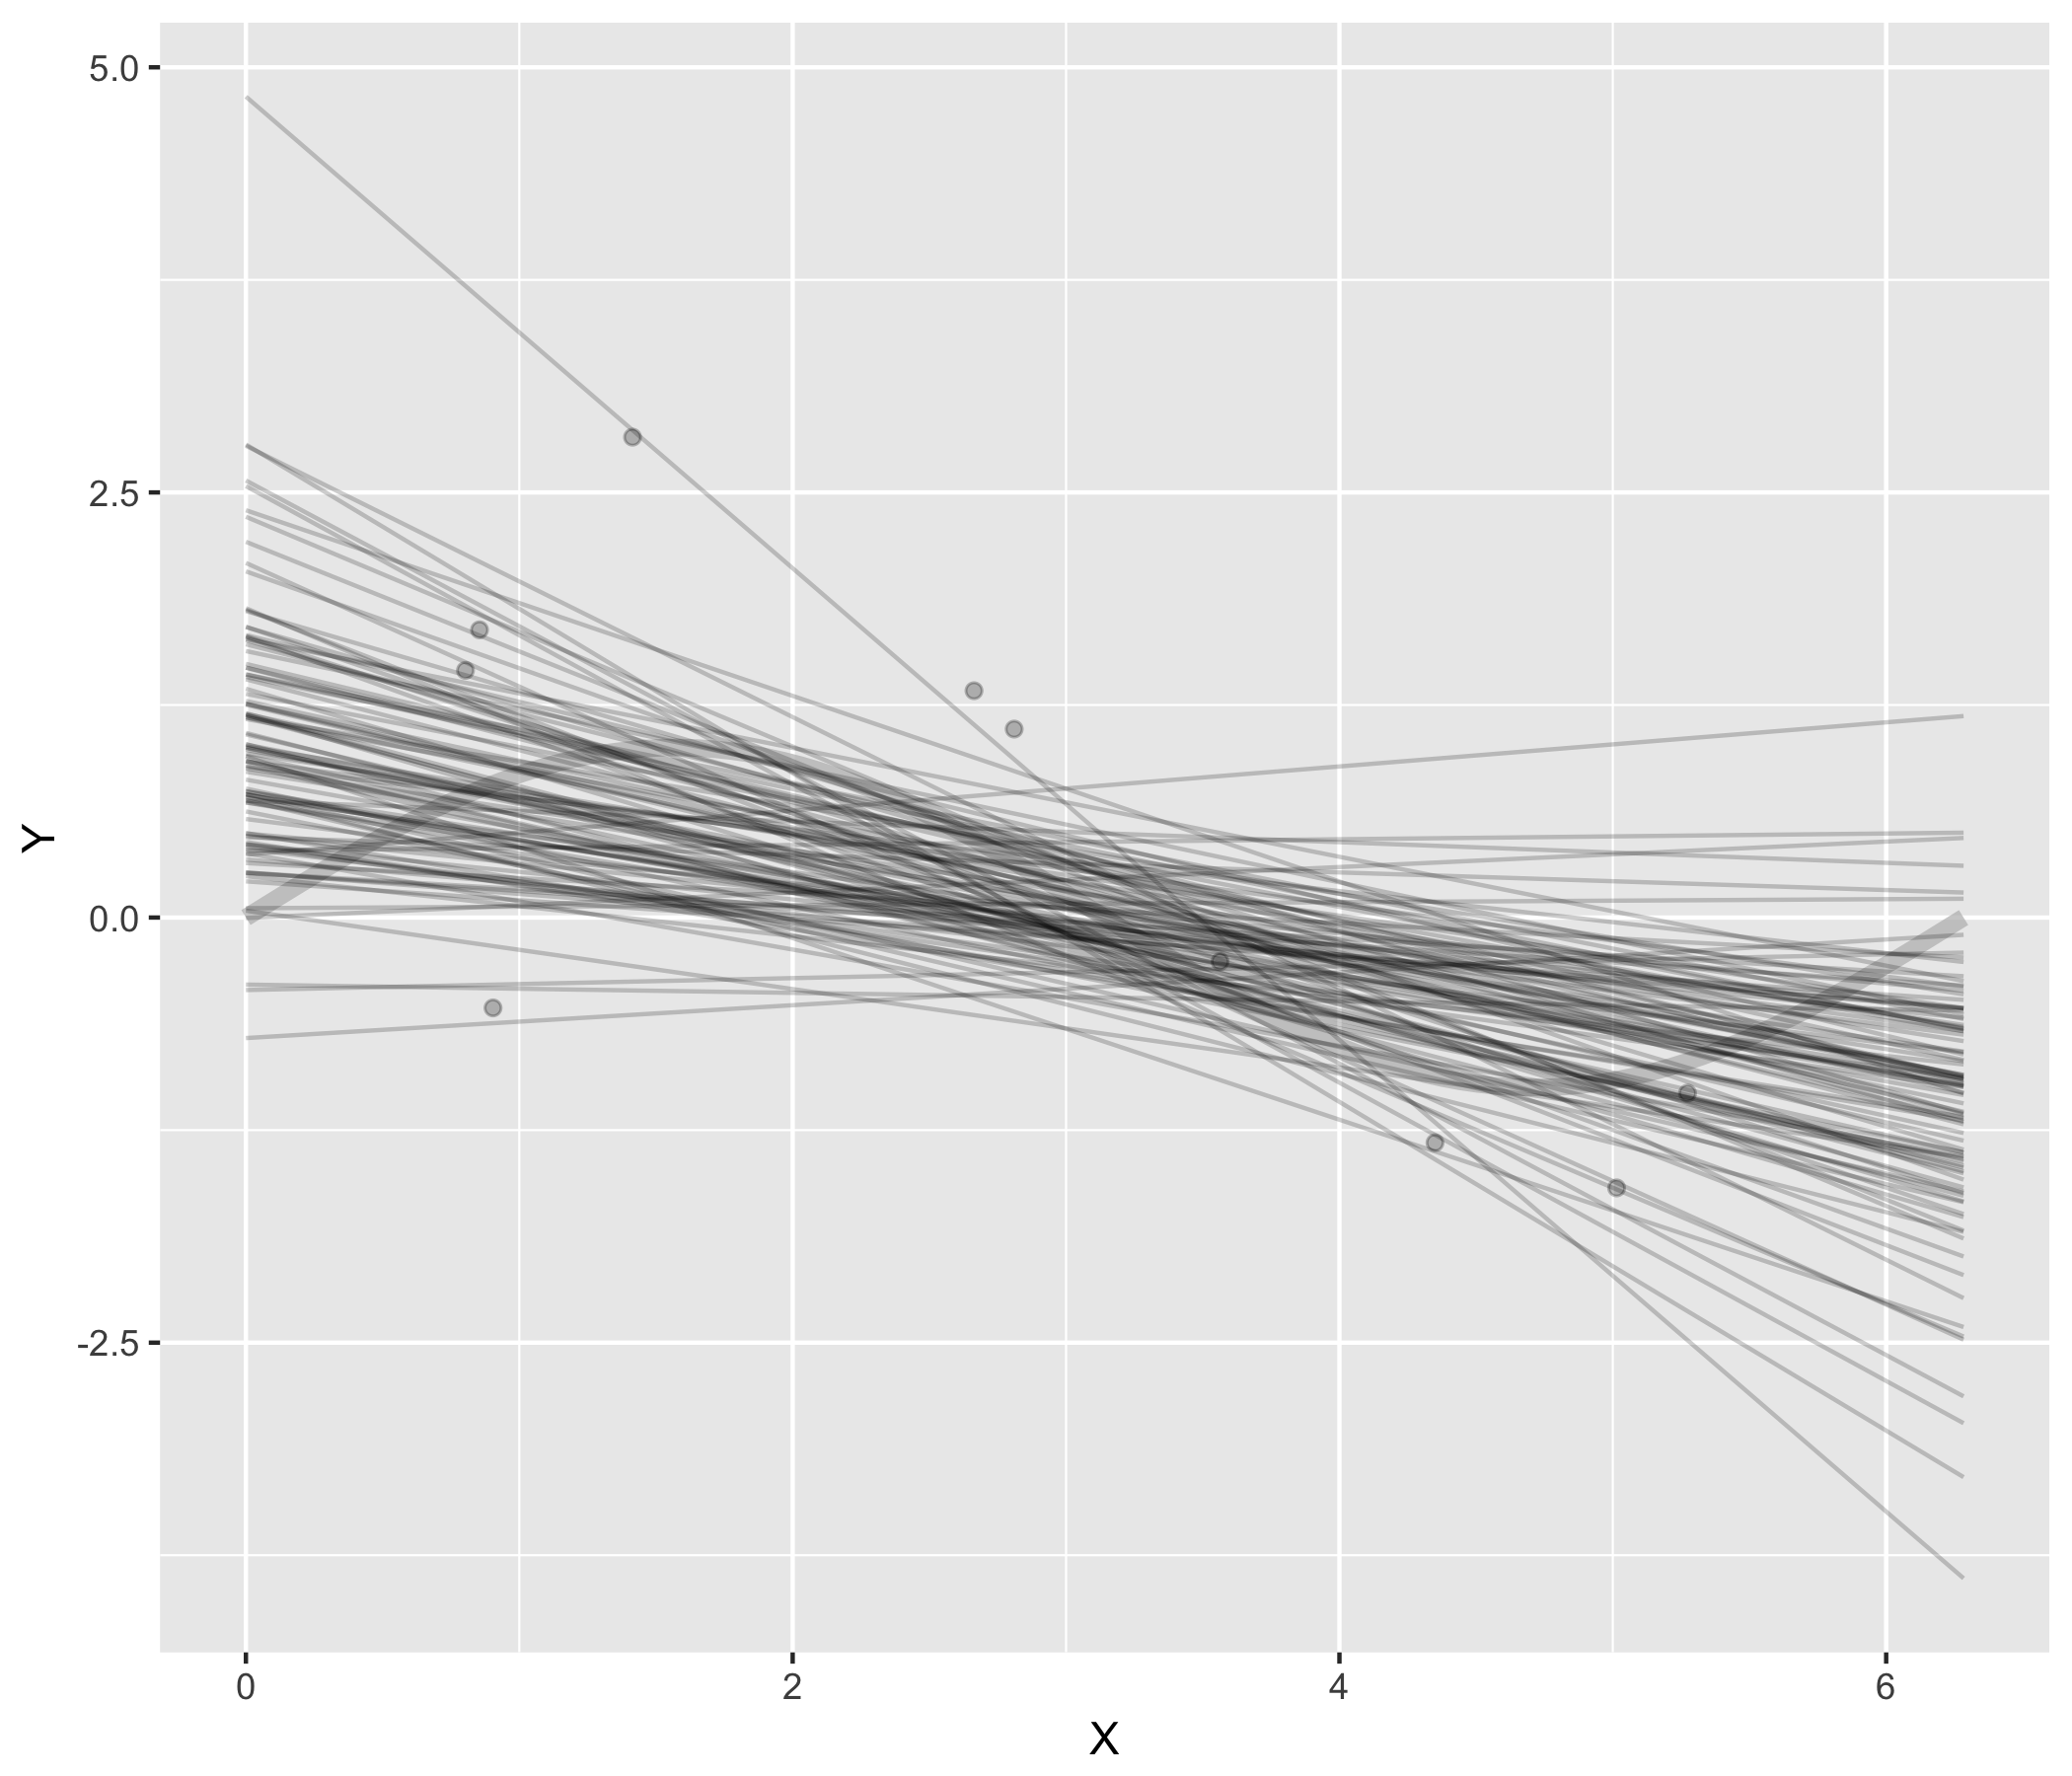
\includegraphics[scale=0.09]{model_variance_less_samples}
  \end{figure}
\end{frame}
%
%
\begin{frame}
  As the amount of data available for training is increased, estimates of
  expected error tend to approach a limit after which they cannot be decreased:
  \begin{figure}
    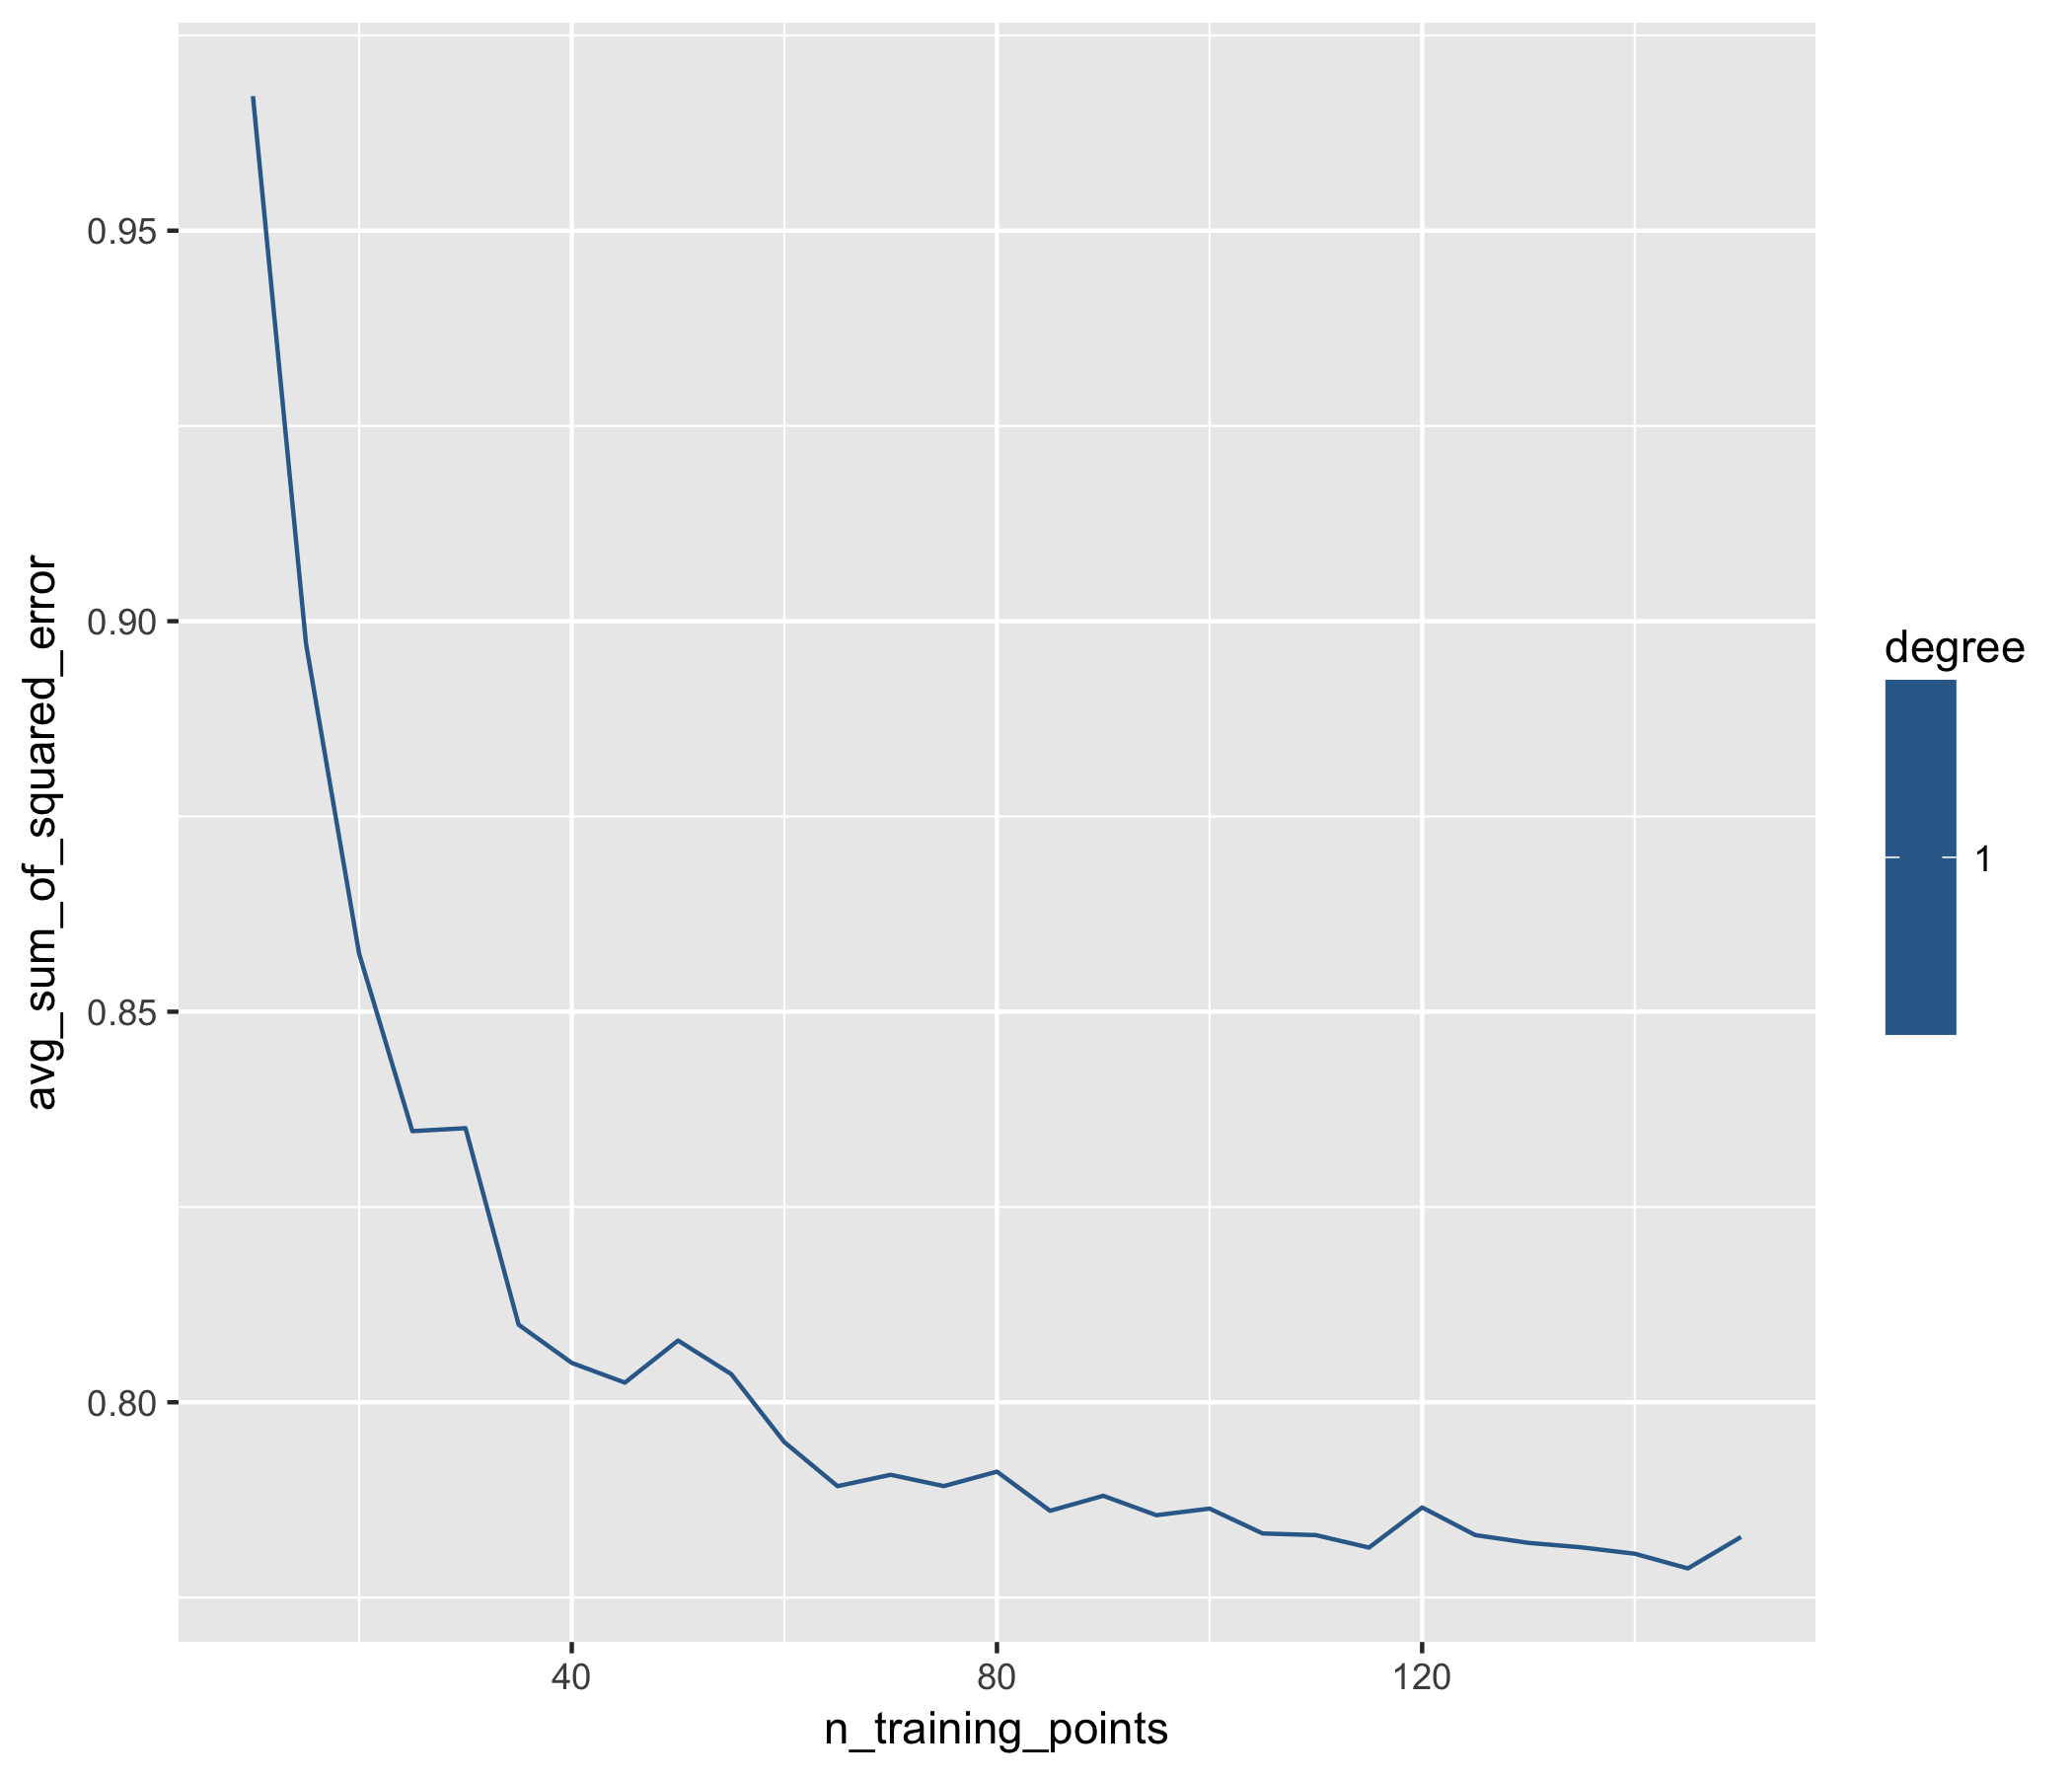
\includegraphics[scale=0.09]{out_of_sample_learning_curve}
  \end{figure}
\end{frame}
%
%
\begin{frame}
  The error remaining after the estimate stabilizes are due to the other error
  components: the irreducible error and the model bias.
  \begin{figure}
    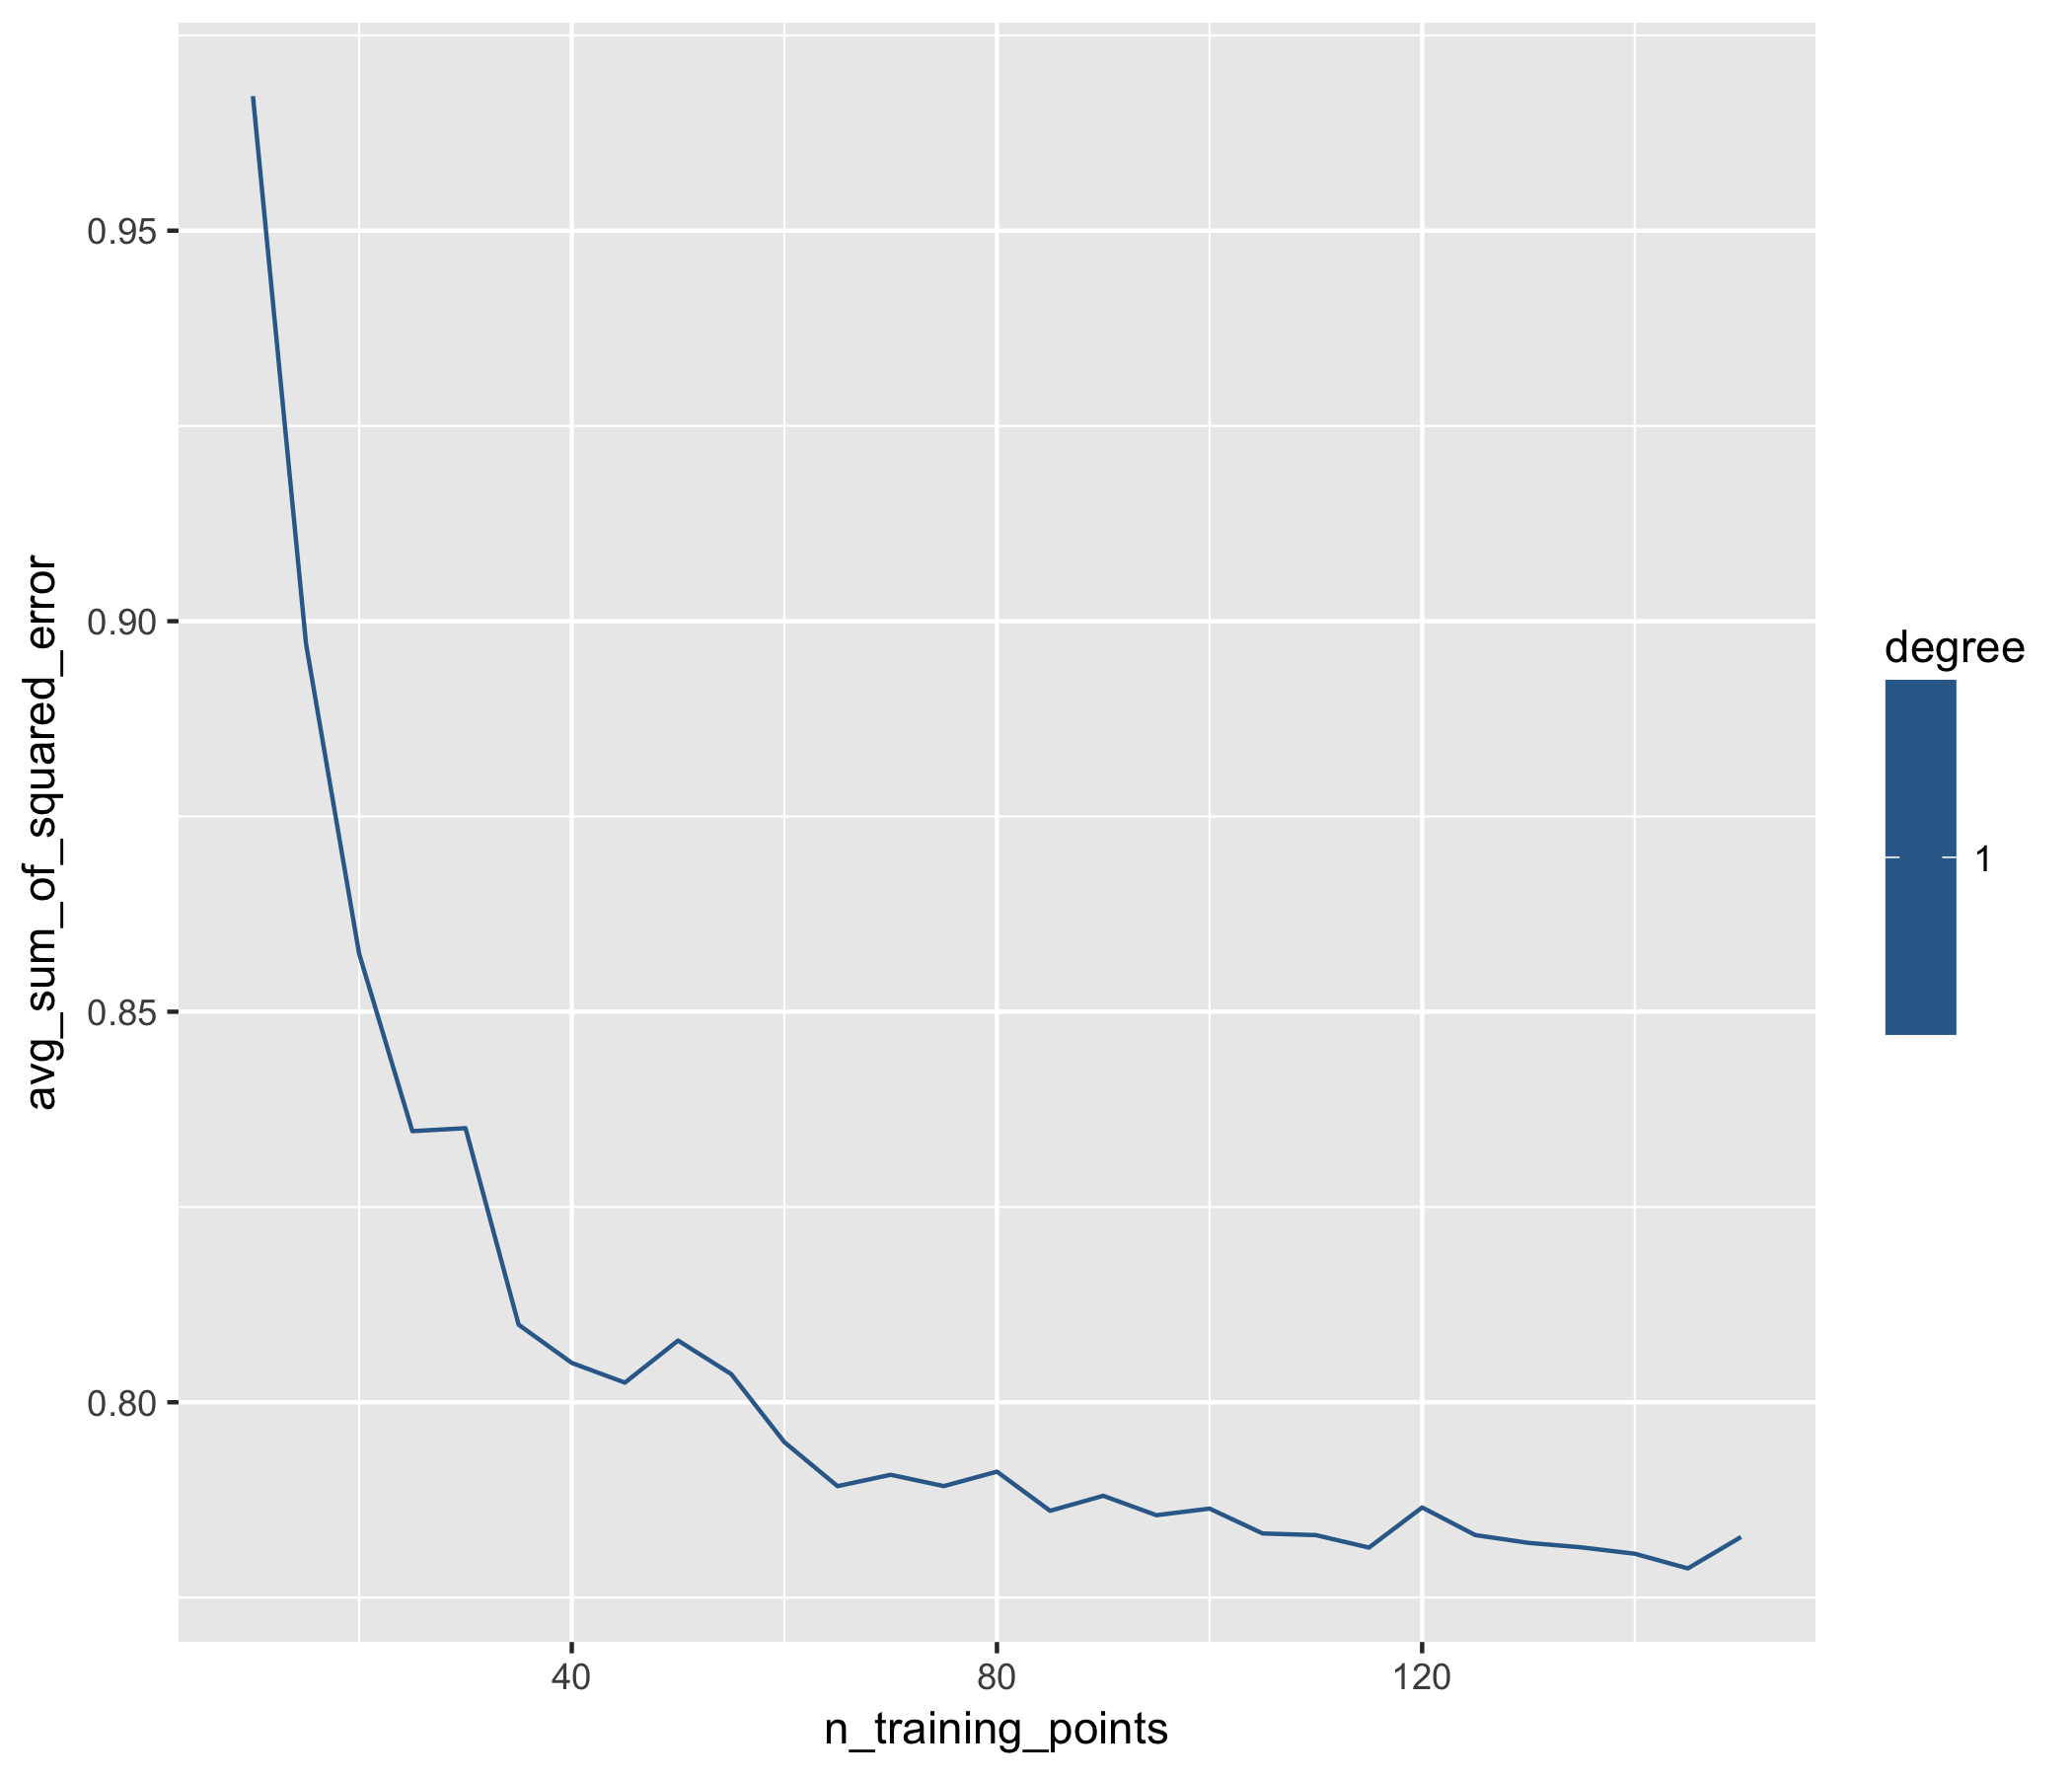
\includegraphics[scale=0.09]{out_of_sample_learning_curve}
  \end{figure}
\end{frame}
%
%
\begin{frame}
  Increasing the complexity of the model also tends to increase the model
  variance:
  \begin{figure}
      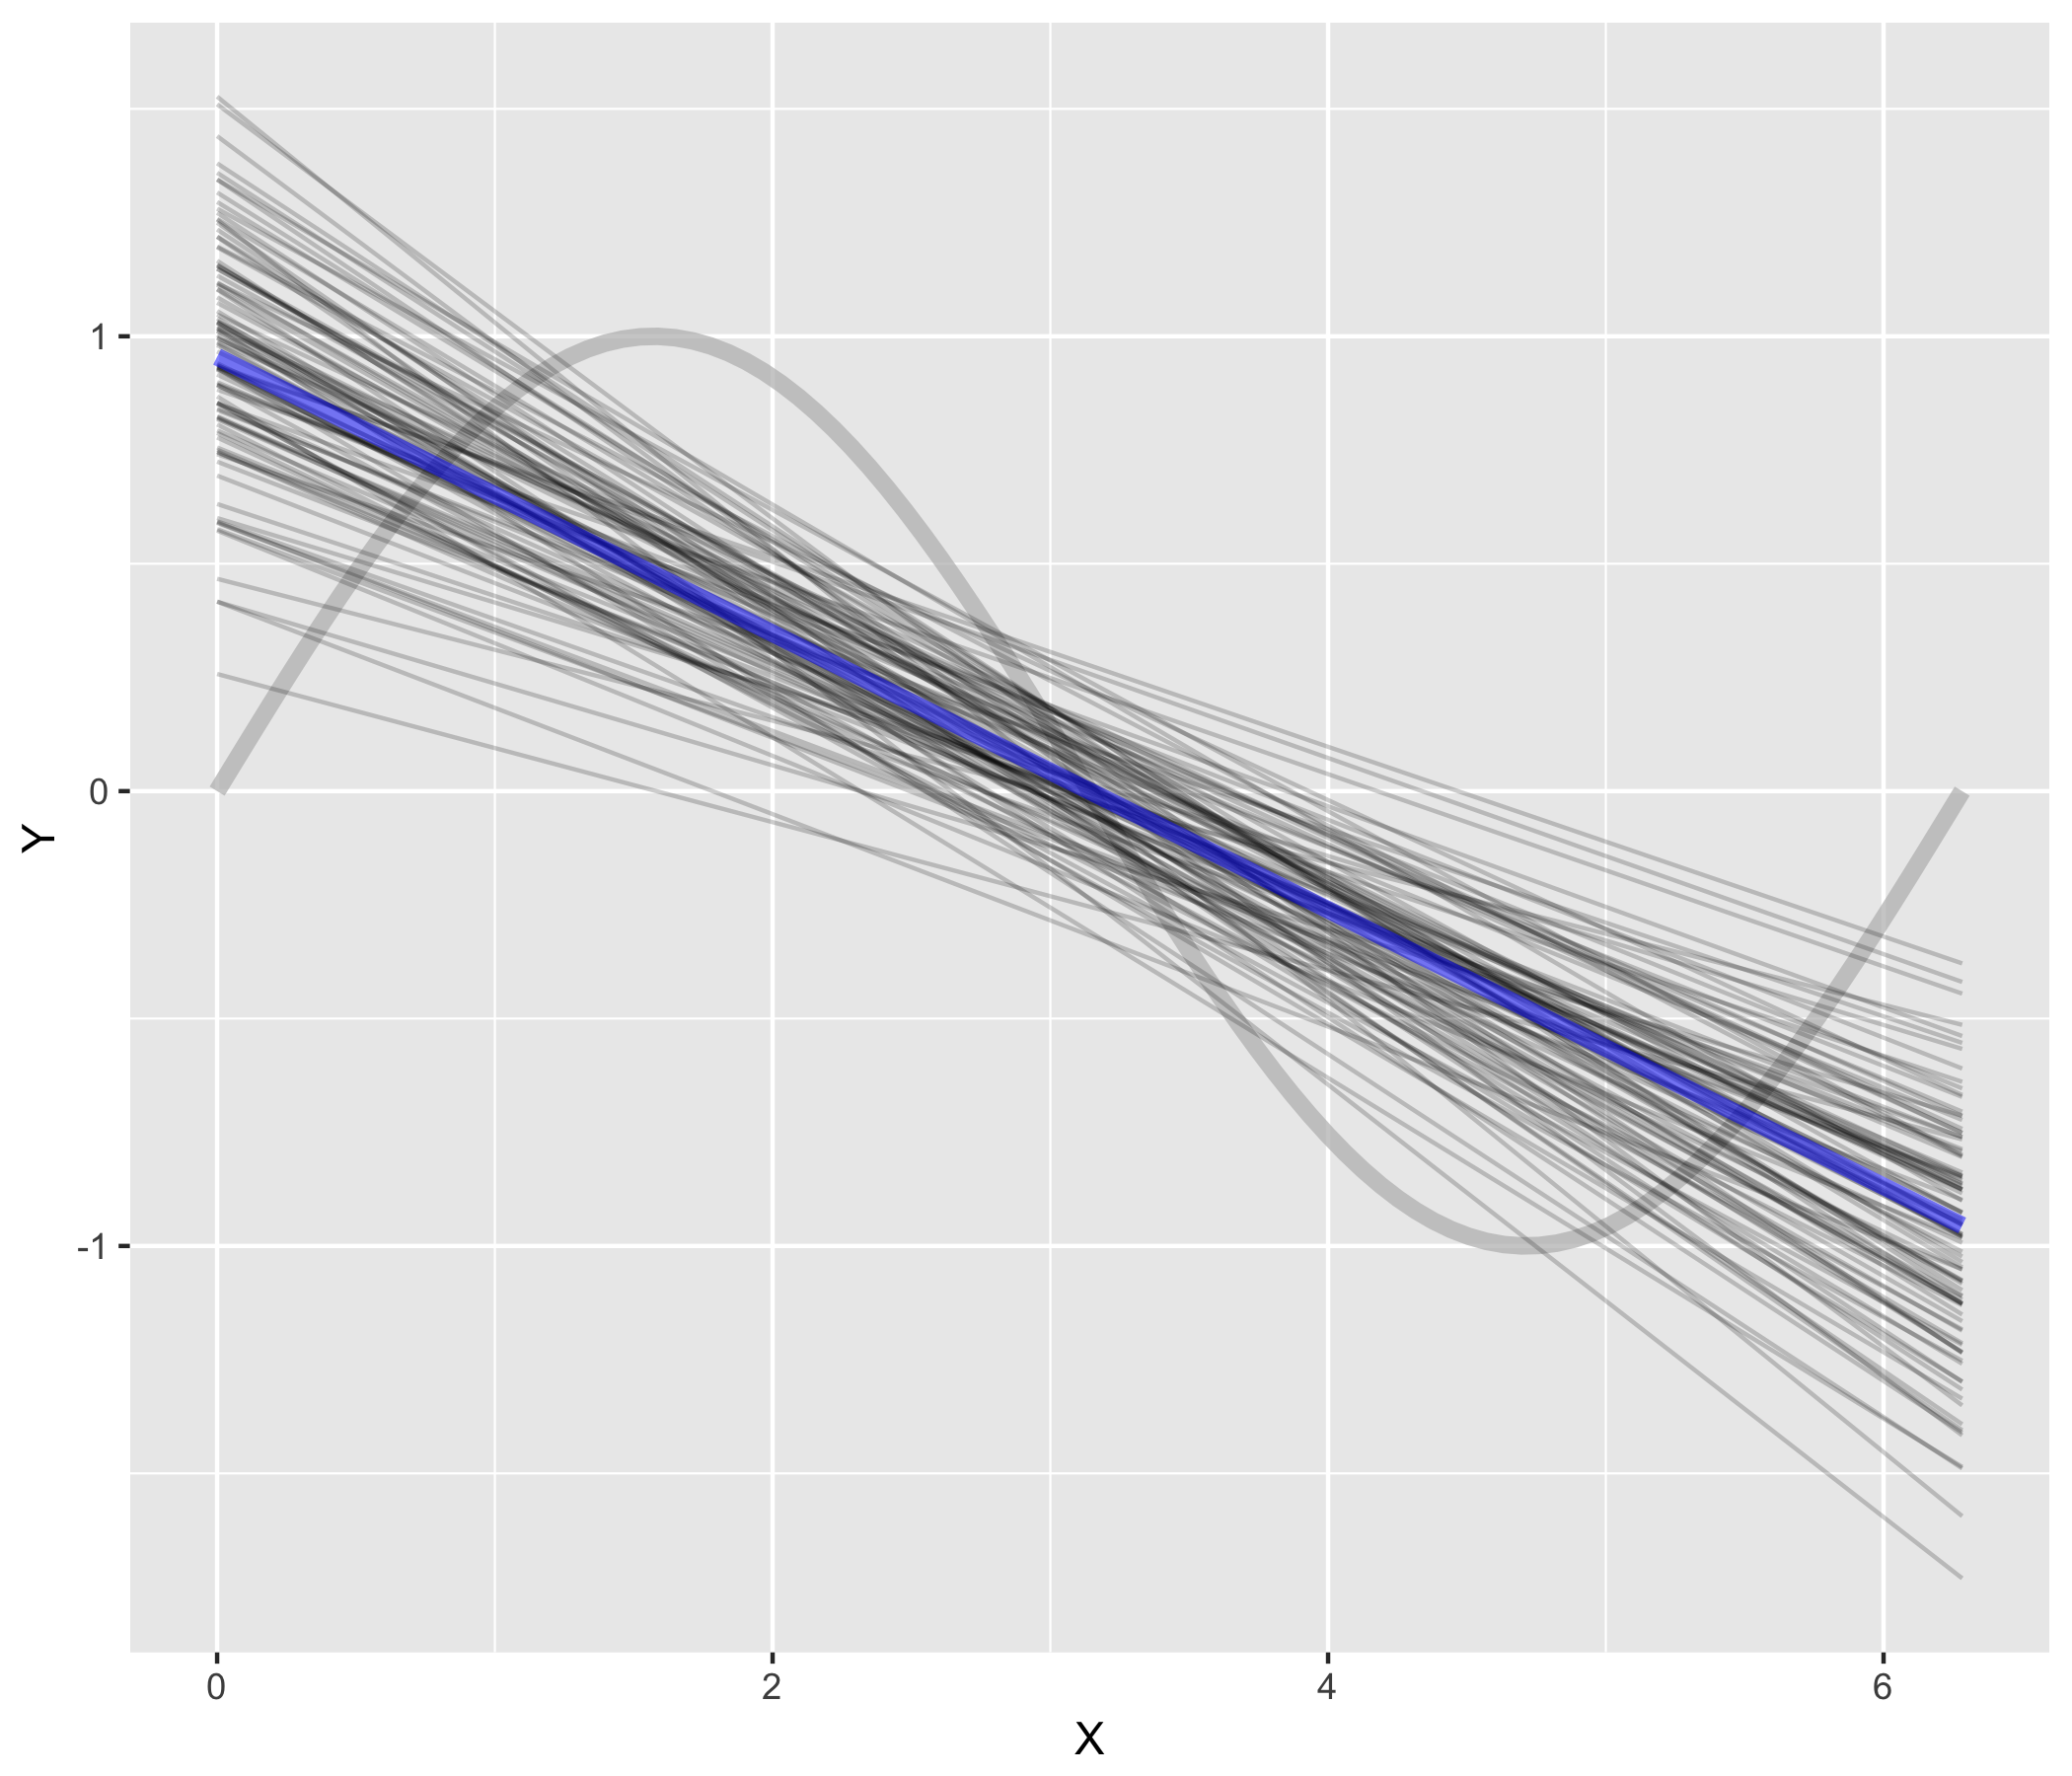
\includegraphics[scale=0.05]{model_variance}
      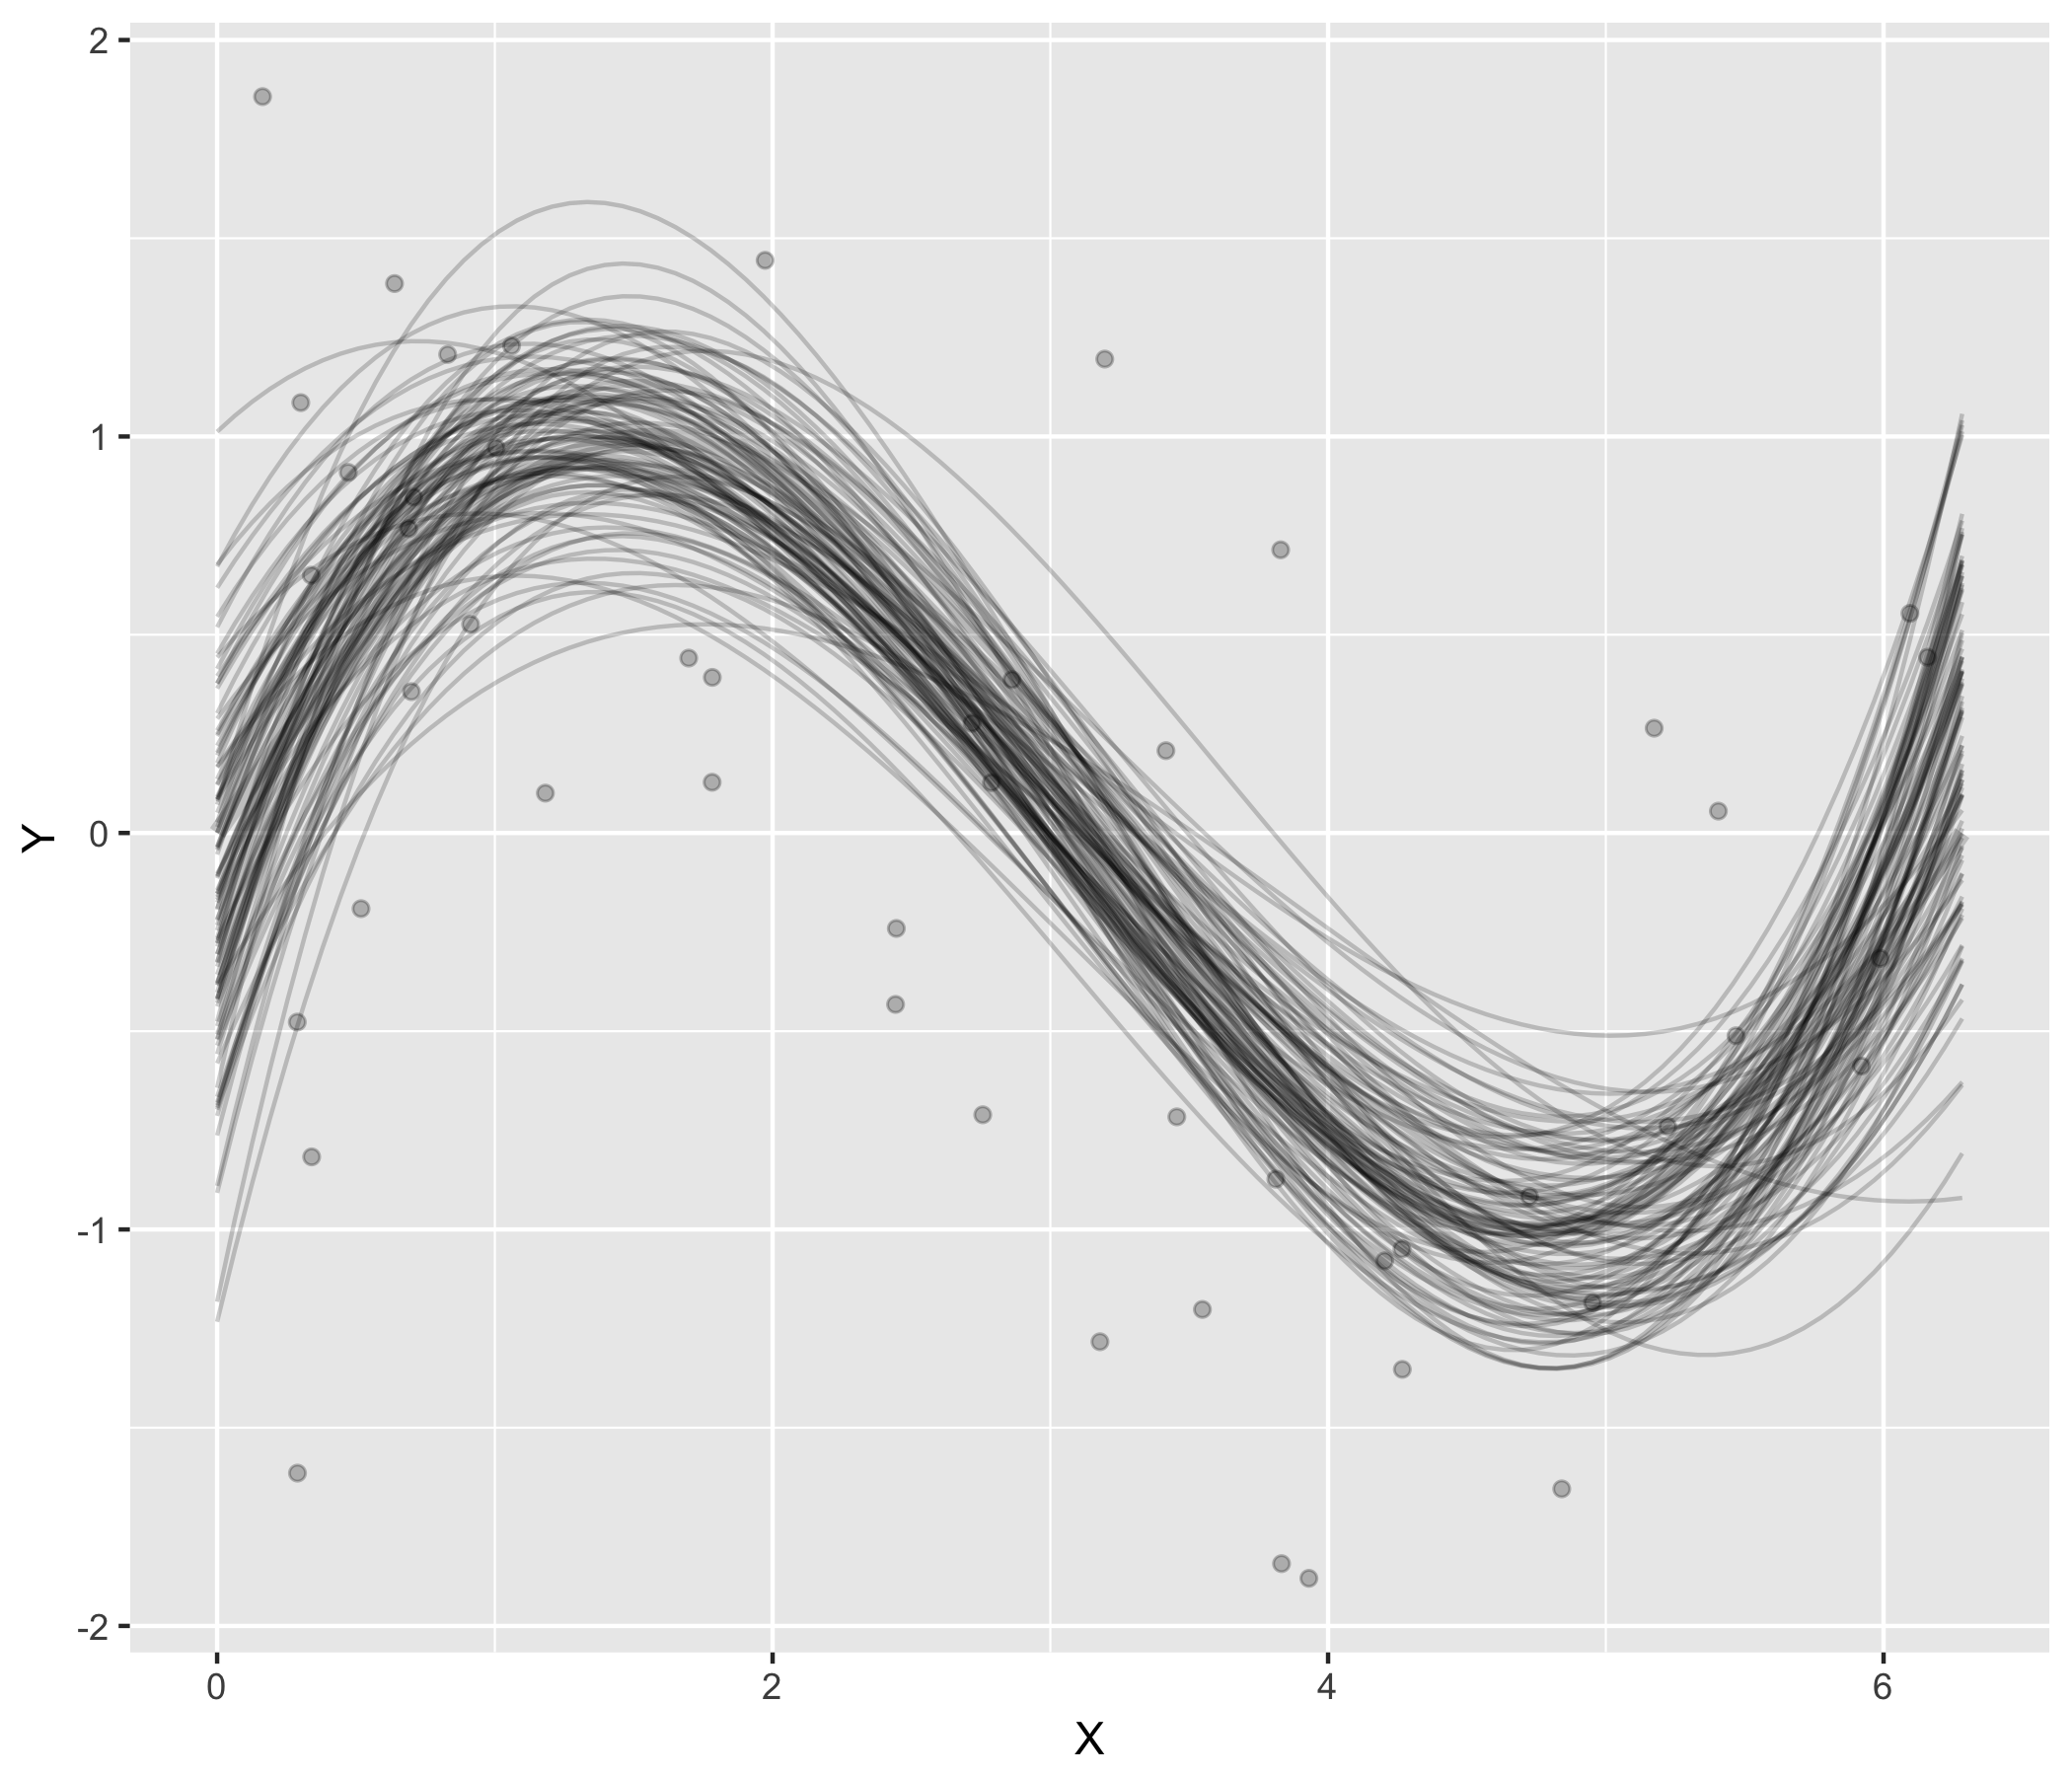
\includegraphics[scale=0.05]{model_variance_cubic}
  \end{figure}
  \begin{figure}
      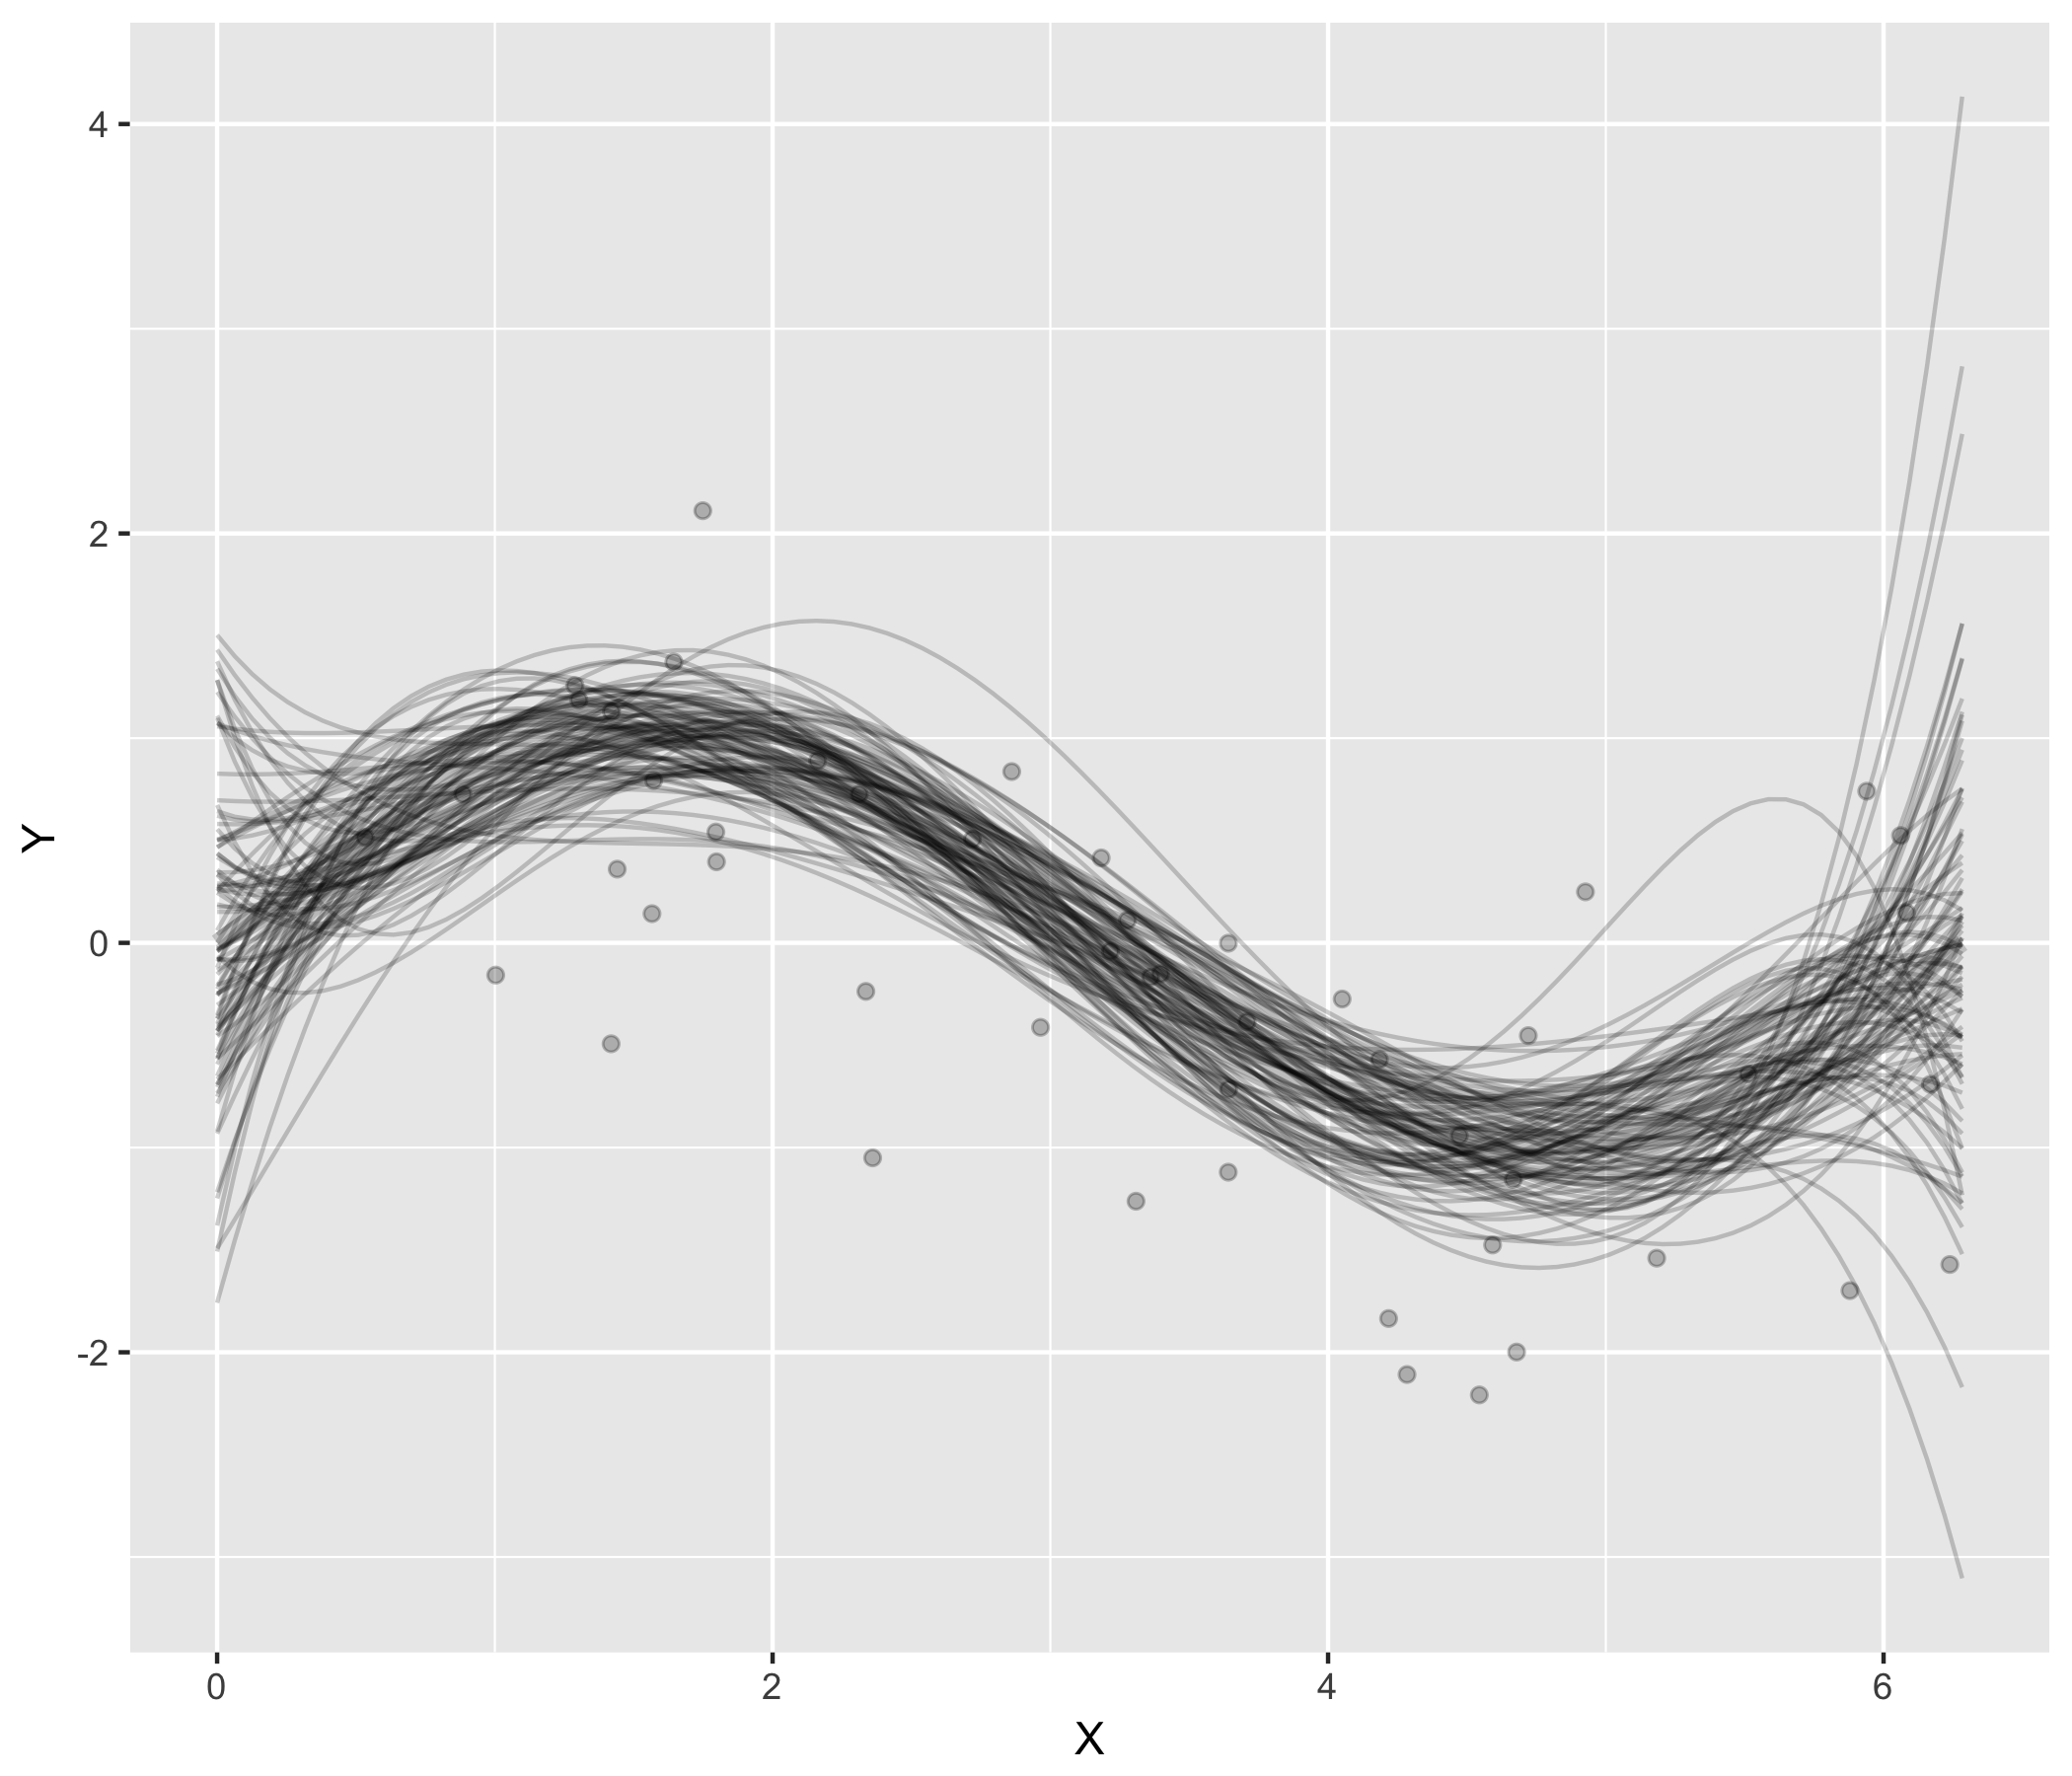
\includegraphics[scale=0.05]{model_variance_quartic}
      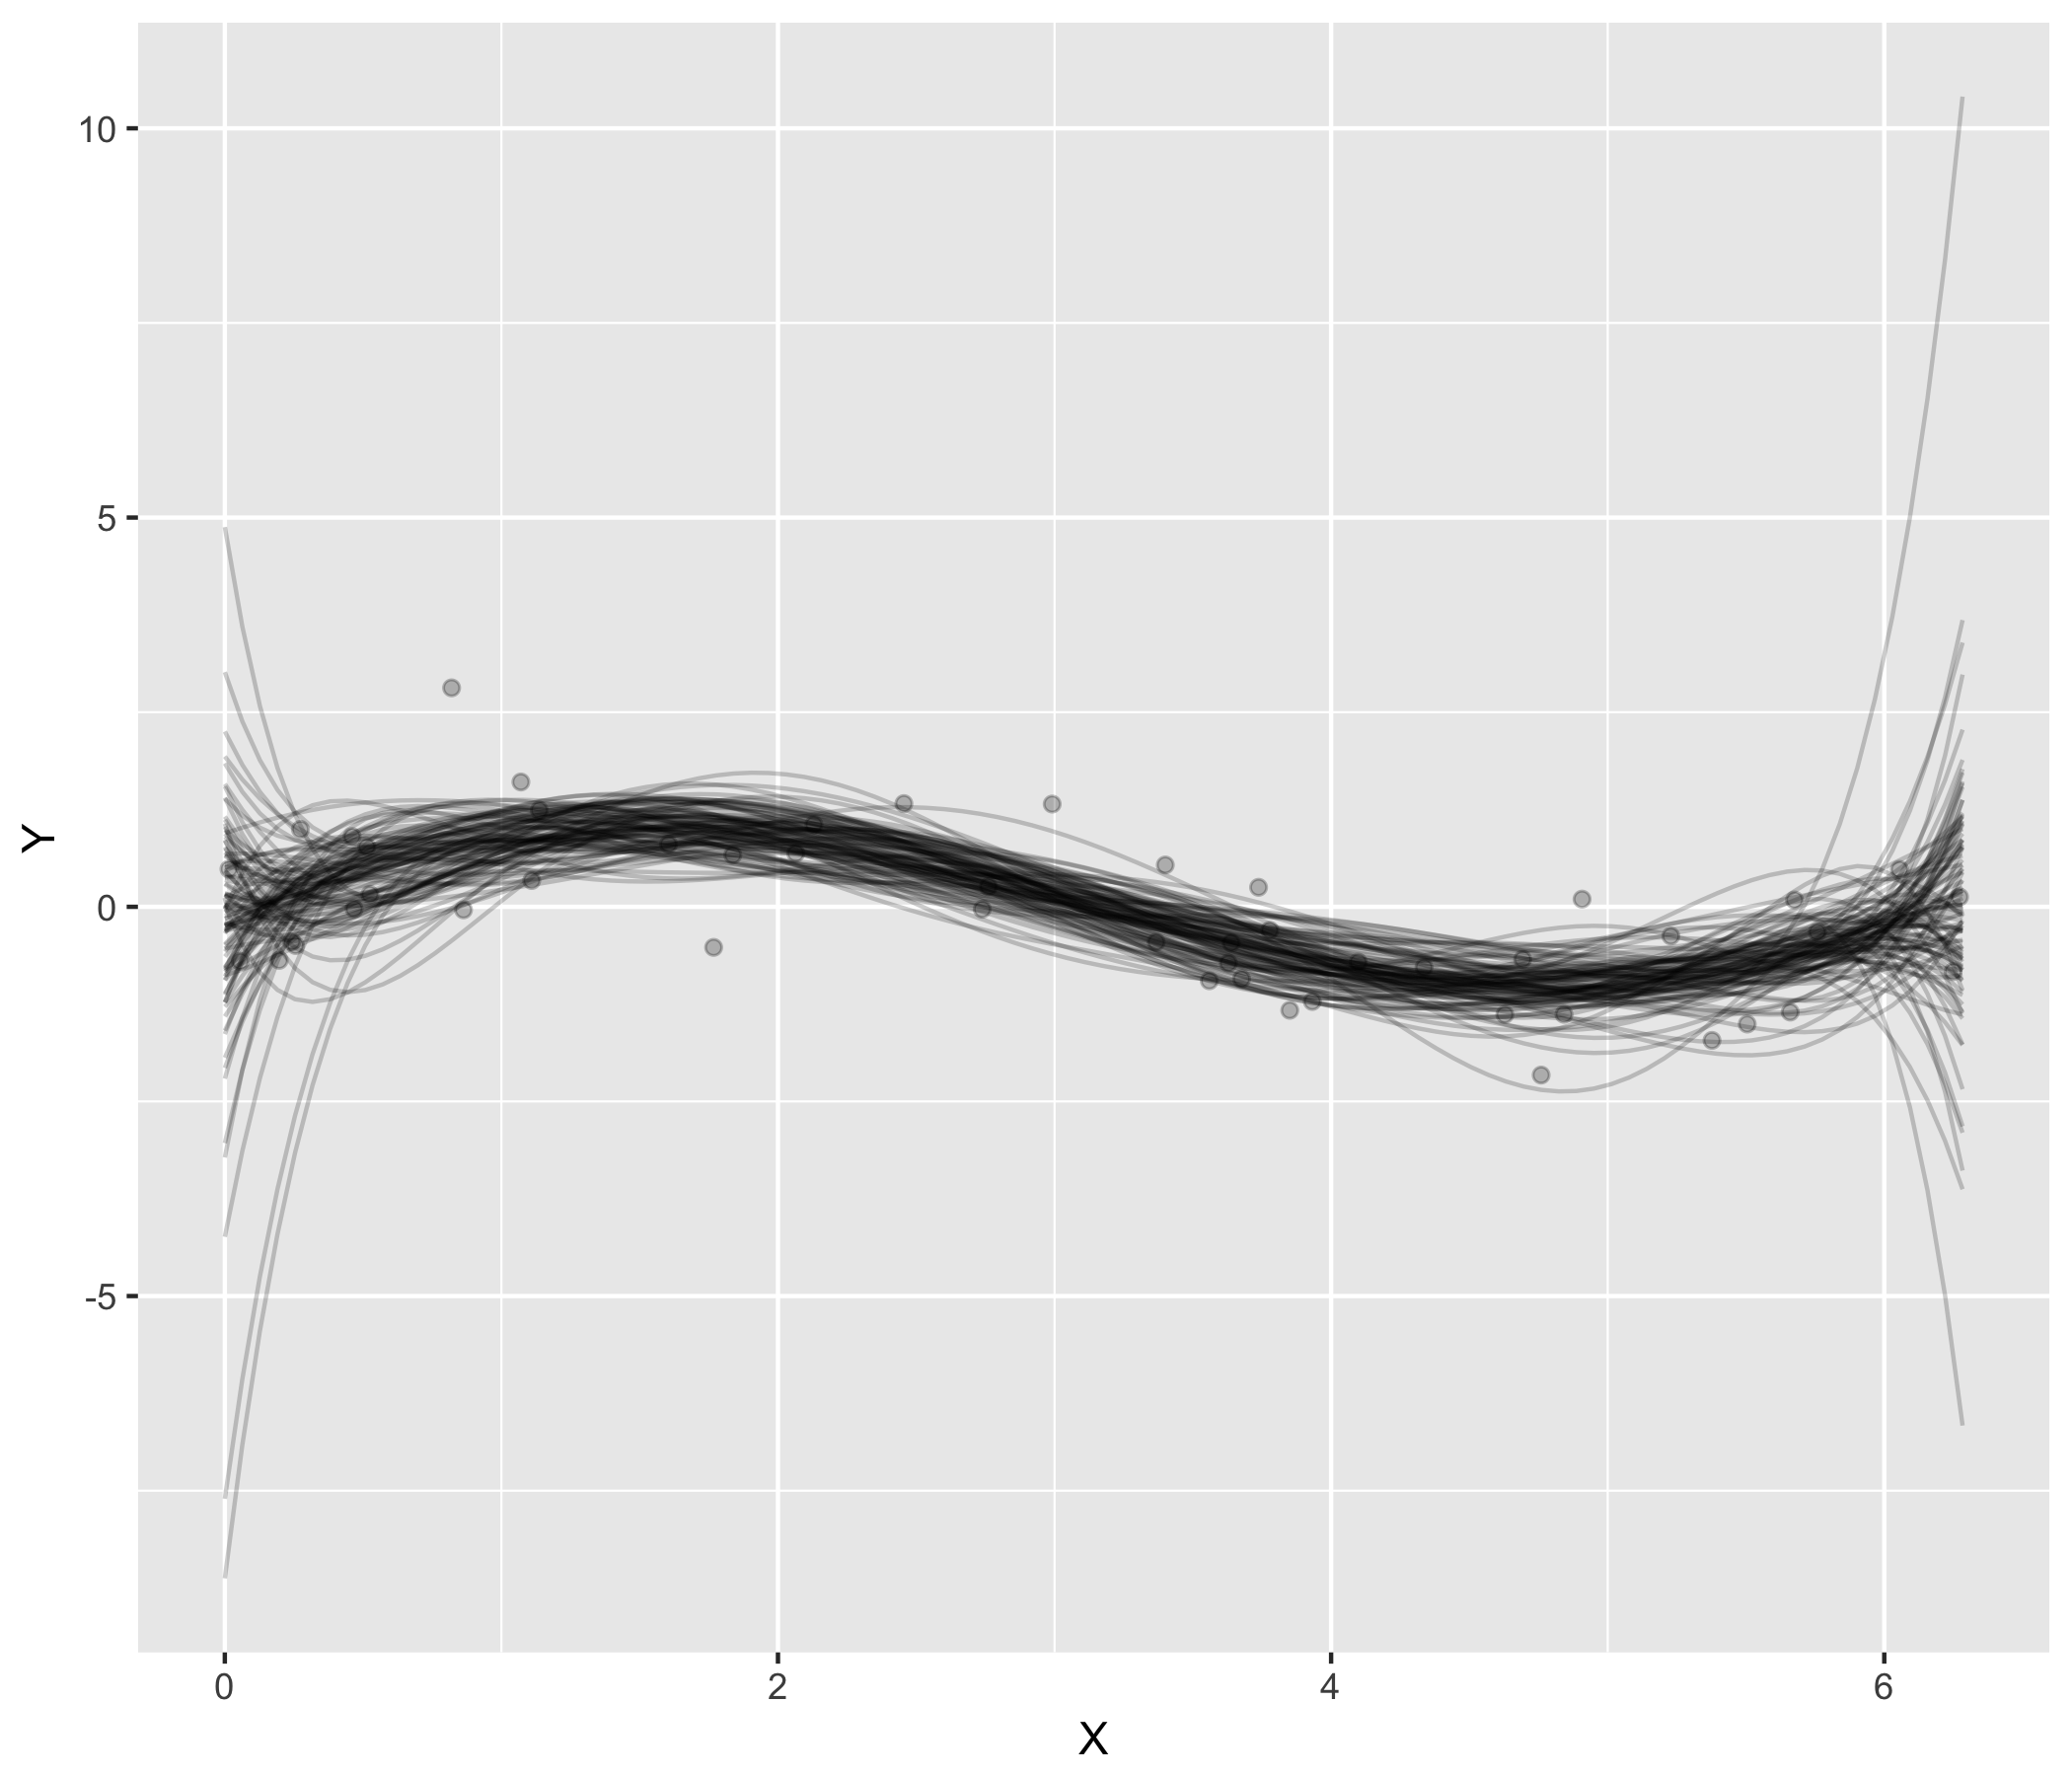
\includegraphics[scale=0.05]{model_variance_septic}
  \end{figure}
\end{frame}
%
%
\begin{frame}
  Near the boundaries of the data the pointwise model variance can be extremely
  large, and dominate the signal:
  \begin{figure}
    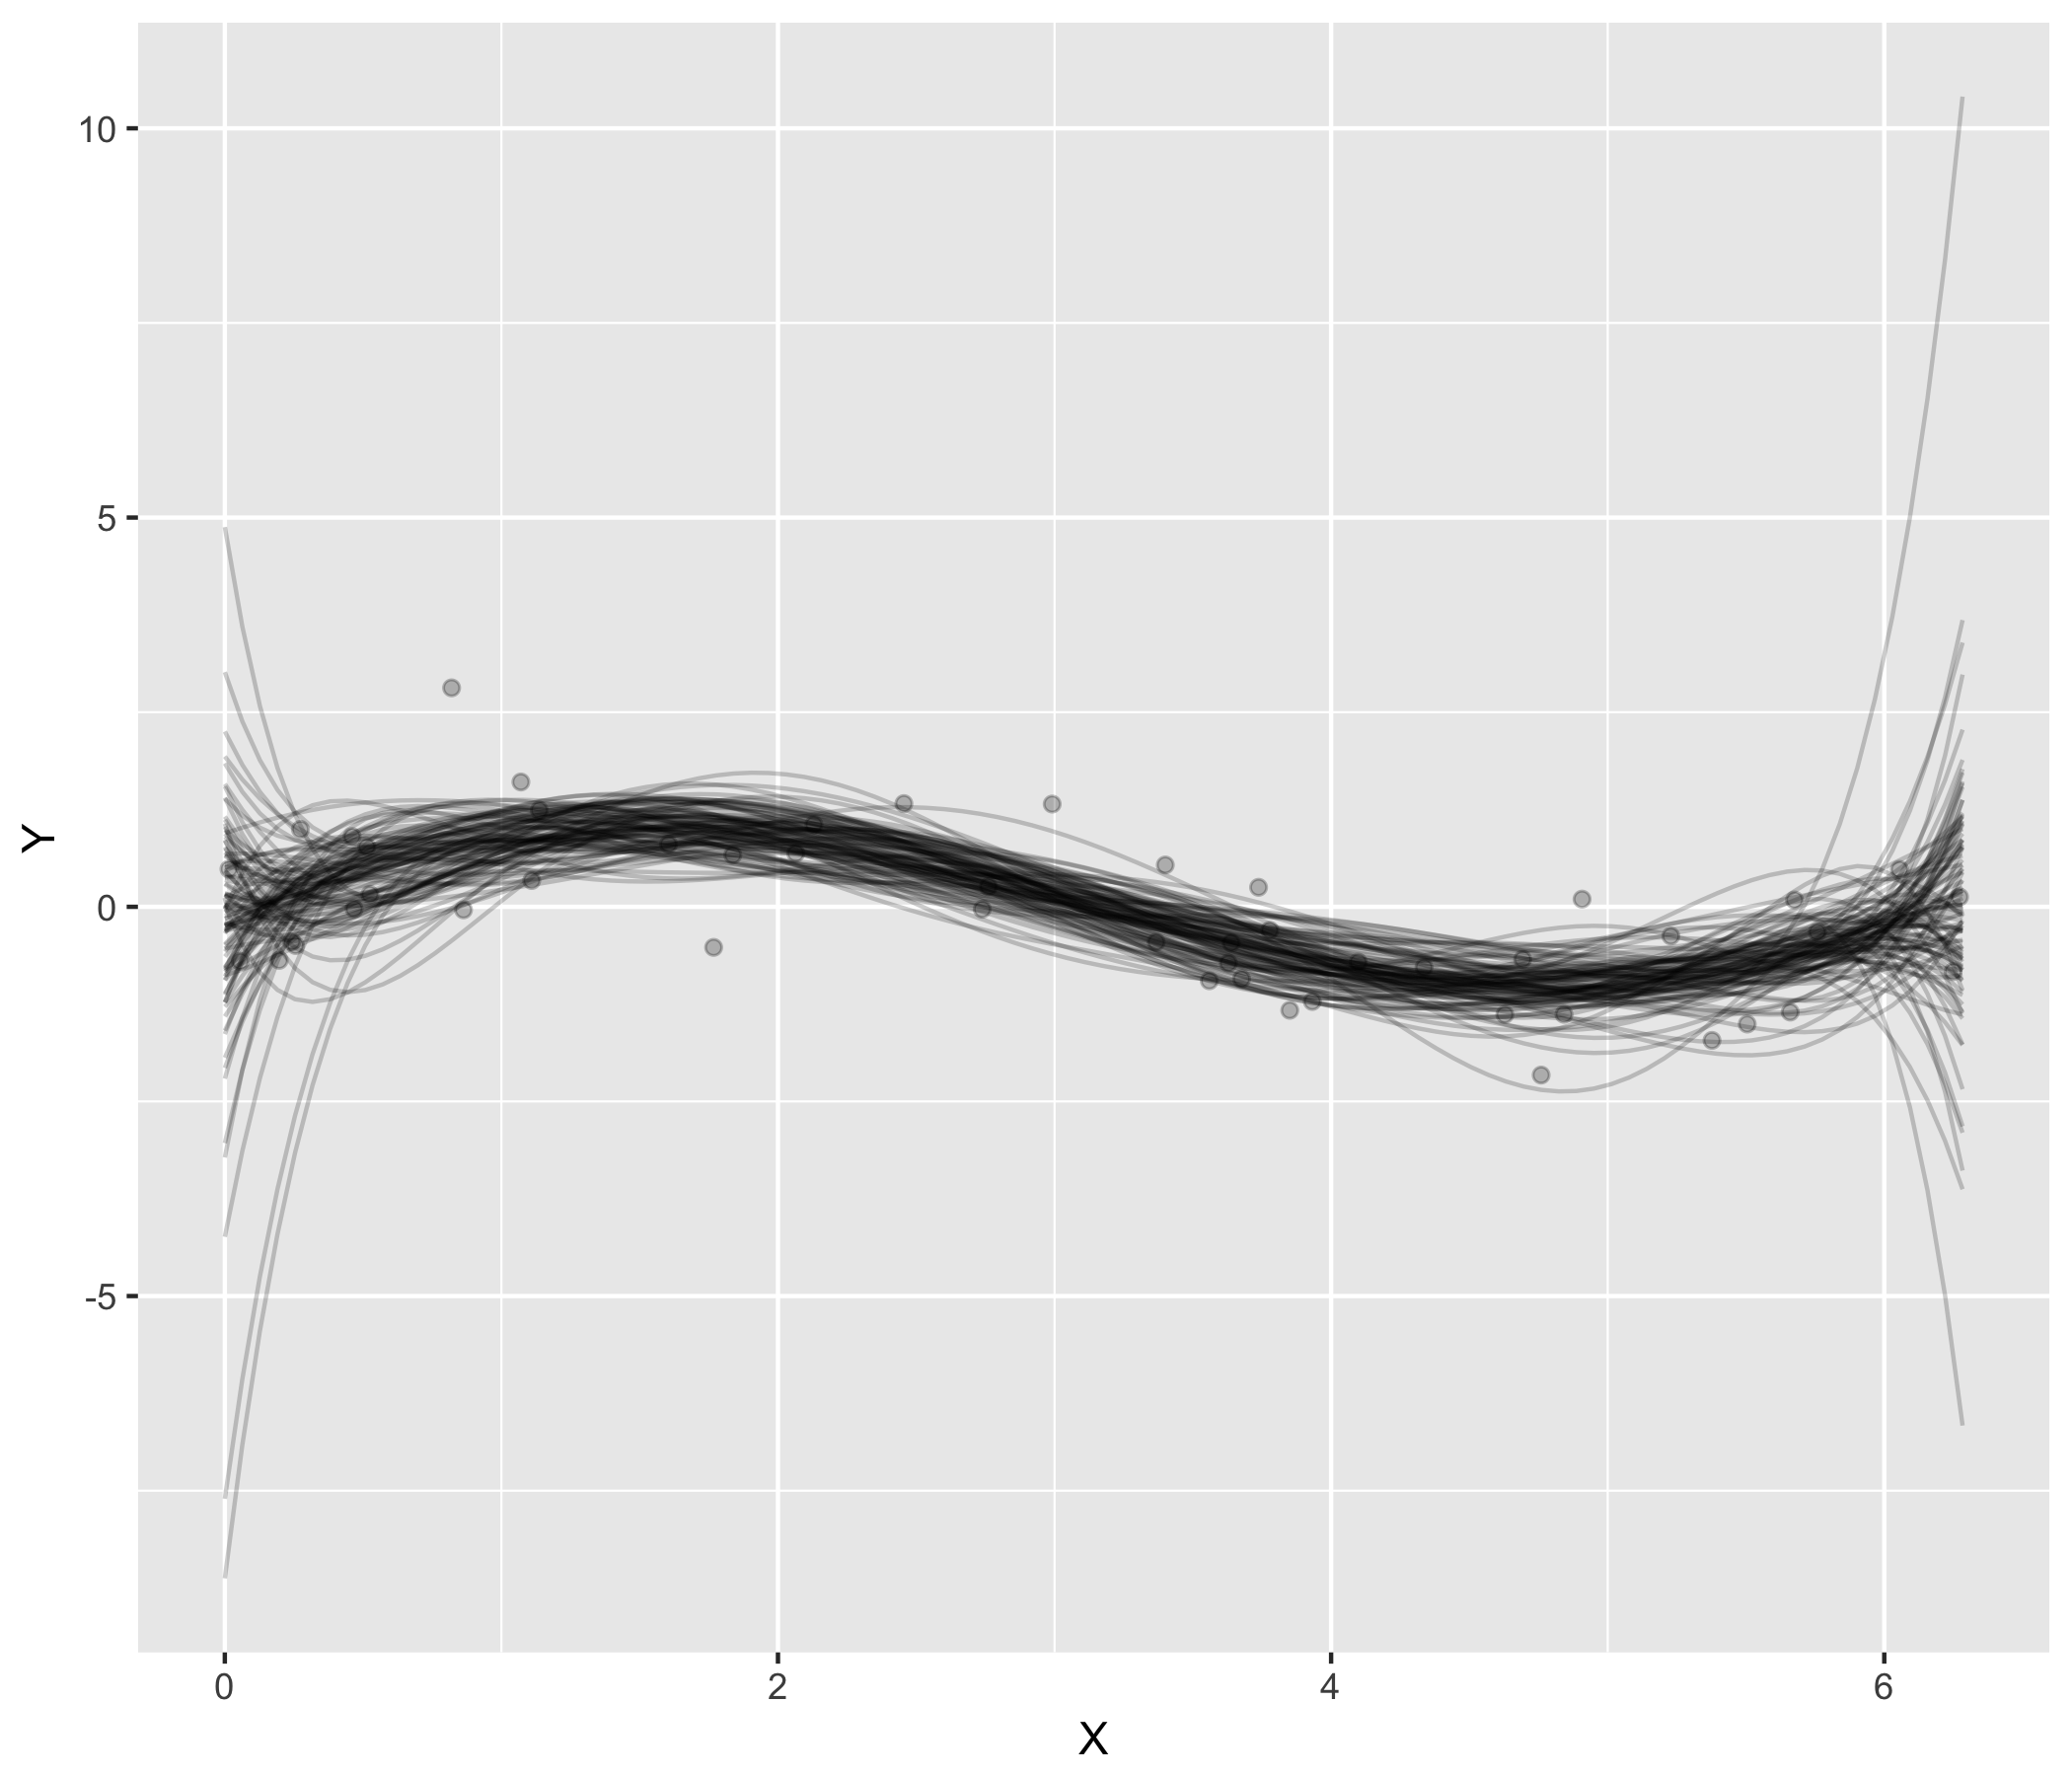
\includegraphics[scale=0.08]{model_variance_septic}
  \end{figure}
\end{frame}
%
%
\begin{frame}
  Increasing the complexity of the model can result in lower bias, and hence a
  lower asymptotic error rate, but enough data is needed to overcome the
  additional model variance:
  \begin{figure}
    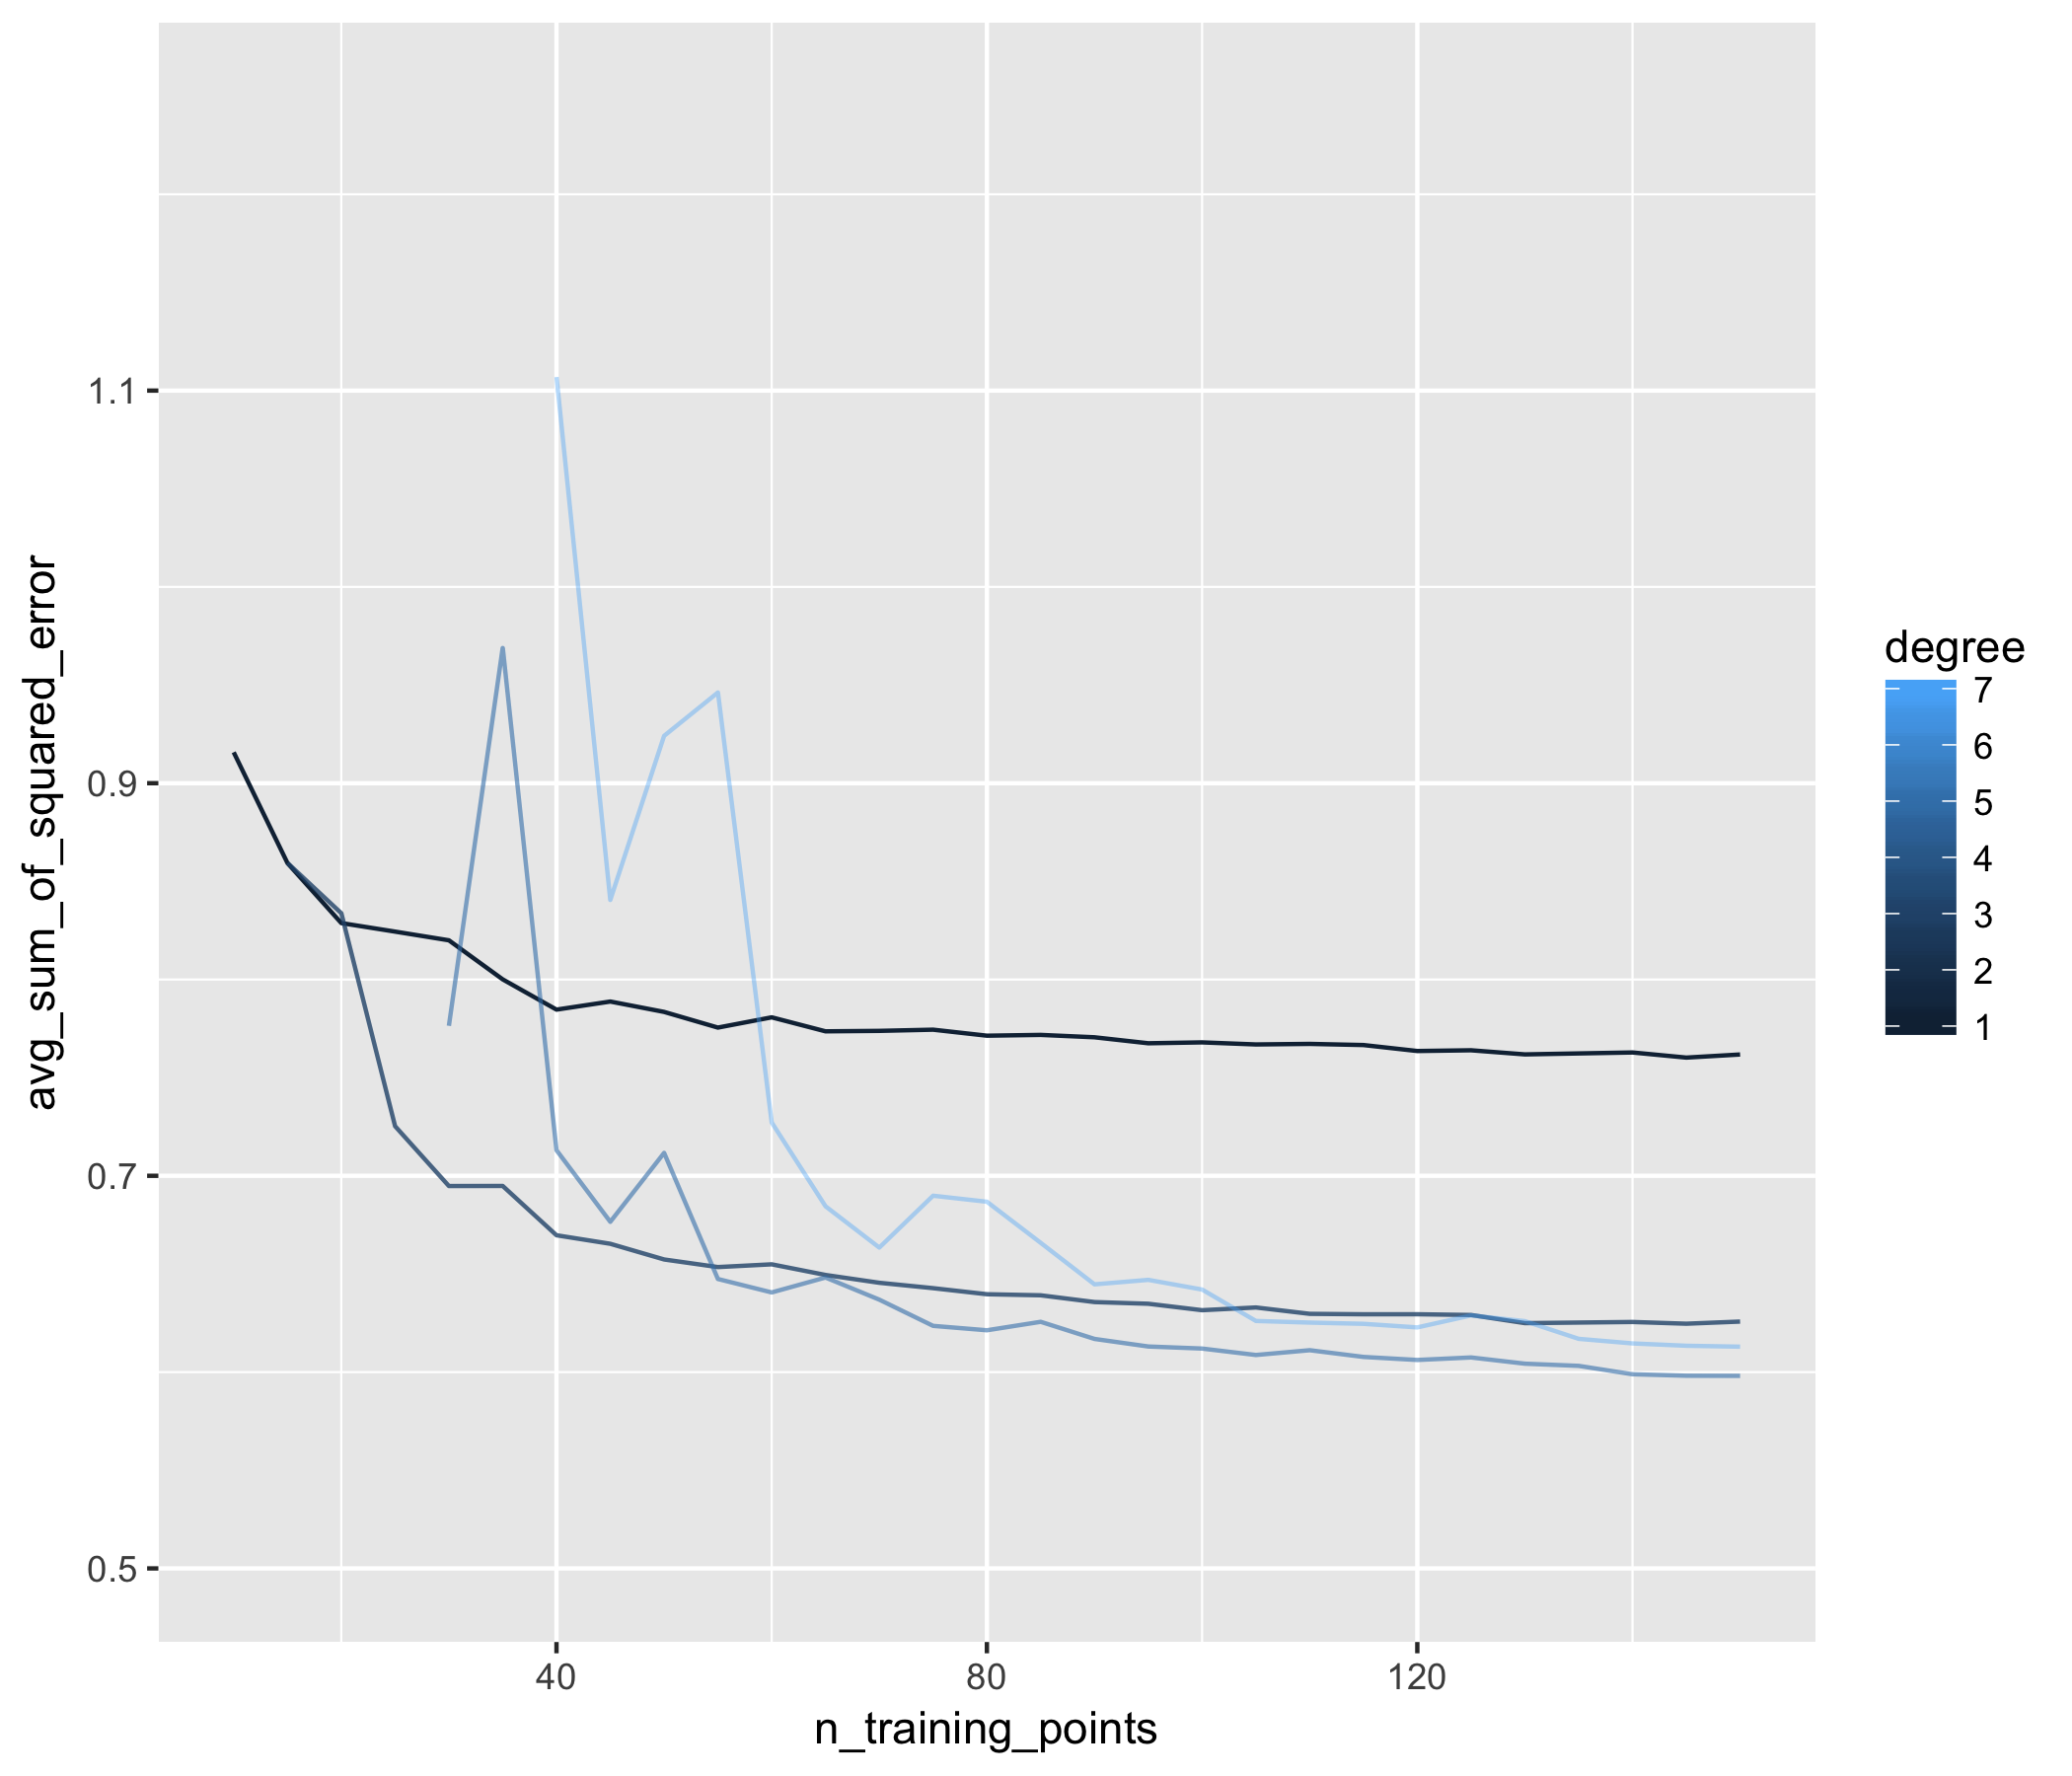
\includegraphics[scale=0.09]{out_of_sample_learning_curves}
  \end{figure}
\end{frame}
%
%
\begin{frame}
  If the complexity is increased too much, the variance can dominate, causing
  the expected error rate to increase
  \begin{figure}
    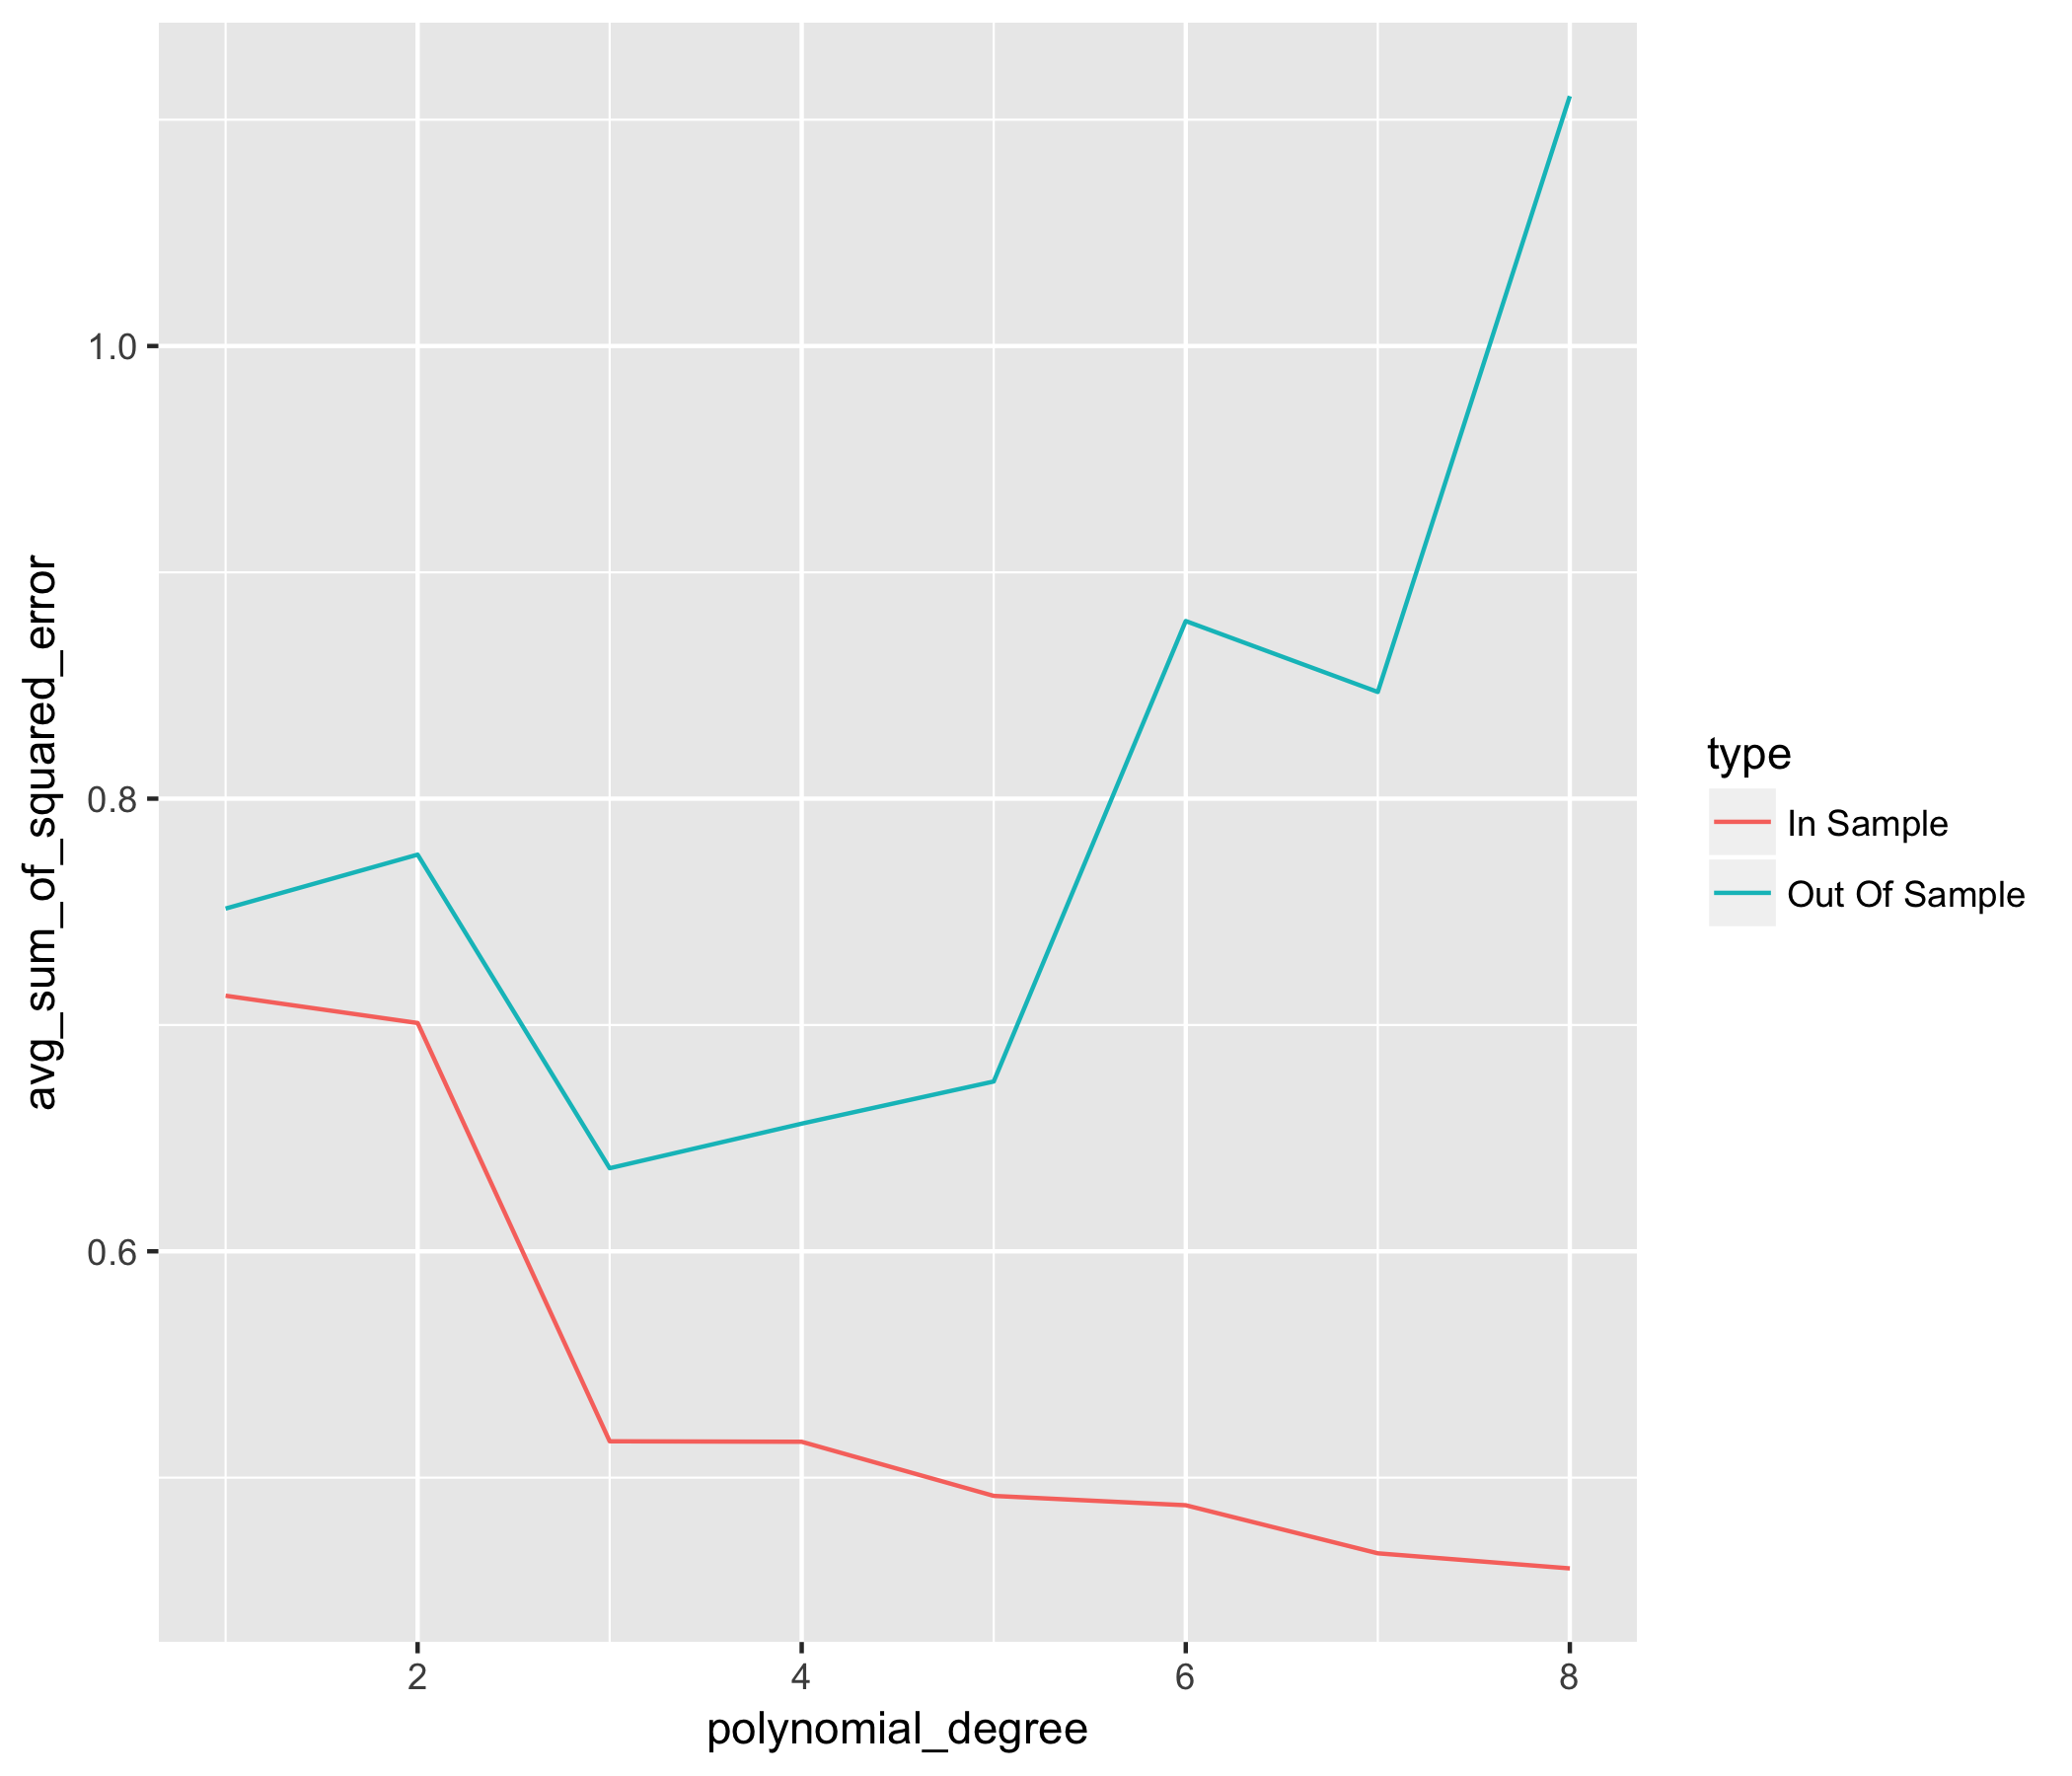
\includegraphics[scale=0.09]{learning_curves_by_degree}
  \end{figure}
\end{frame}
%
%
\begin{frame}
  Finally, increasing the irreducible error rate also increases the model variance:
  \begin{figure}
    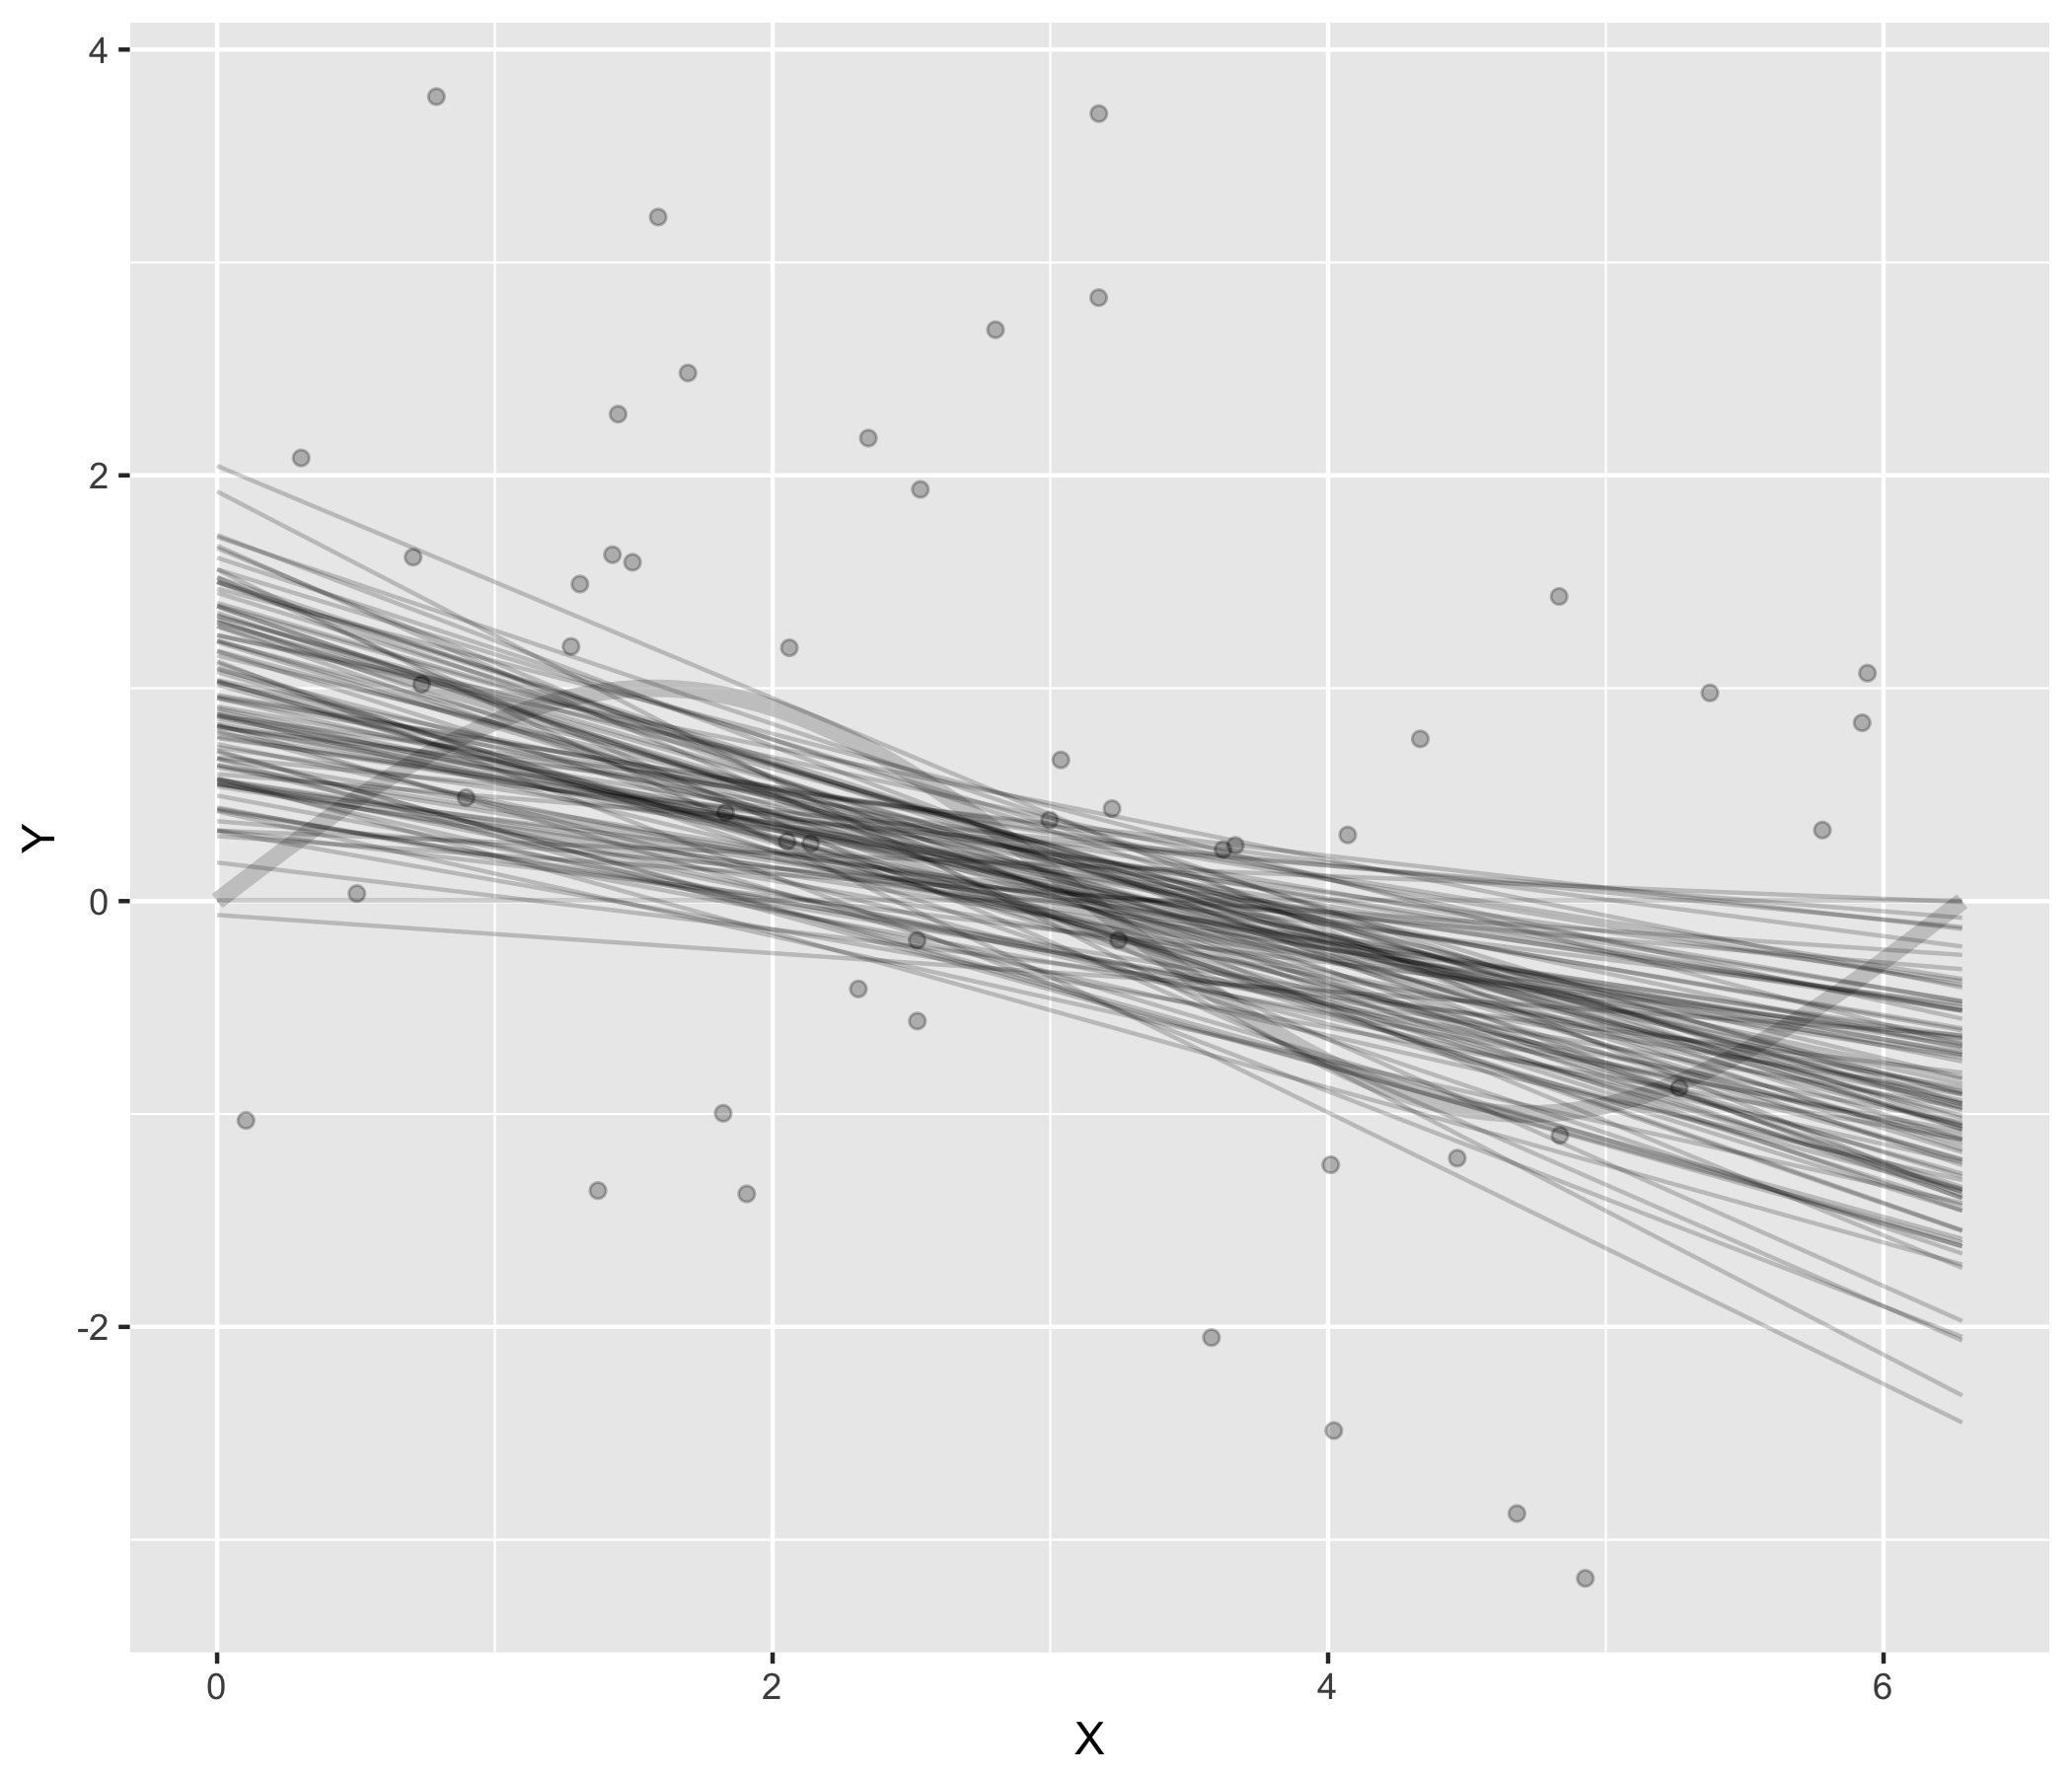
\includegraphics[scale=0.09]{model_variance_more_error}
  \end{figure}
\end{frame}
%
%
\begin{frame}
  A point derived from this discussion is especially important.  The complexity
  of a model should be a function of the \textbf{quantity} and \textbf{quality}
  of the data available.
  \begin{itemize}
    \item \textbf{Quantity}: The variance is a function of the number of samples
    available to train.
    \item \textbf{Quality}: The variance is a function of the irreducible error rate.
  \end{itemize}
\end{frame}
%
%gt
\begin{frame}
  The complexity of a model specification should \textbf{not} be based on
  supposed apriori knowledge of the complexity of the signal function, as
  seductive as this impulse is.
\end{frame}
%
%
\begin{frame}
  This is demonstrated here:
  \begin{figure}
    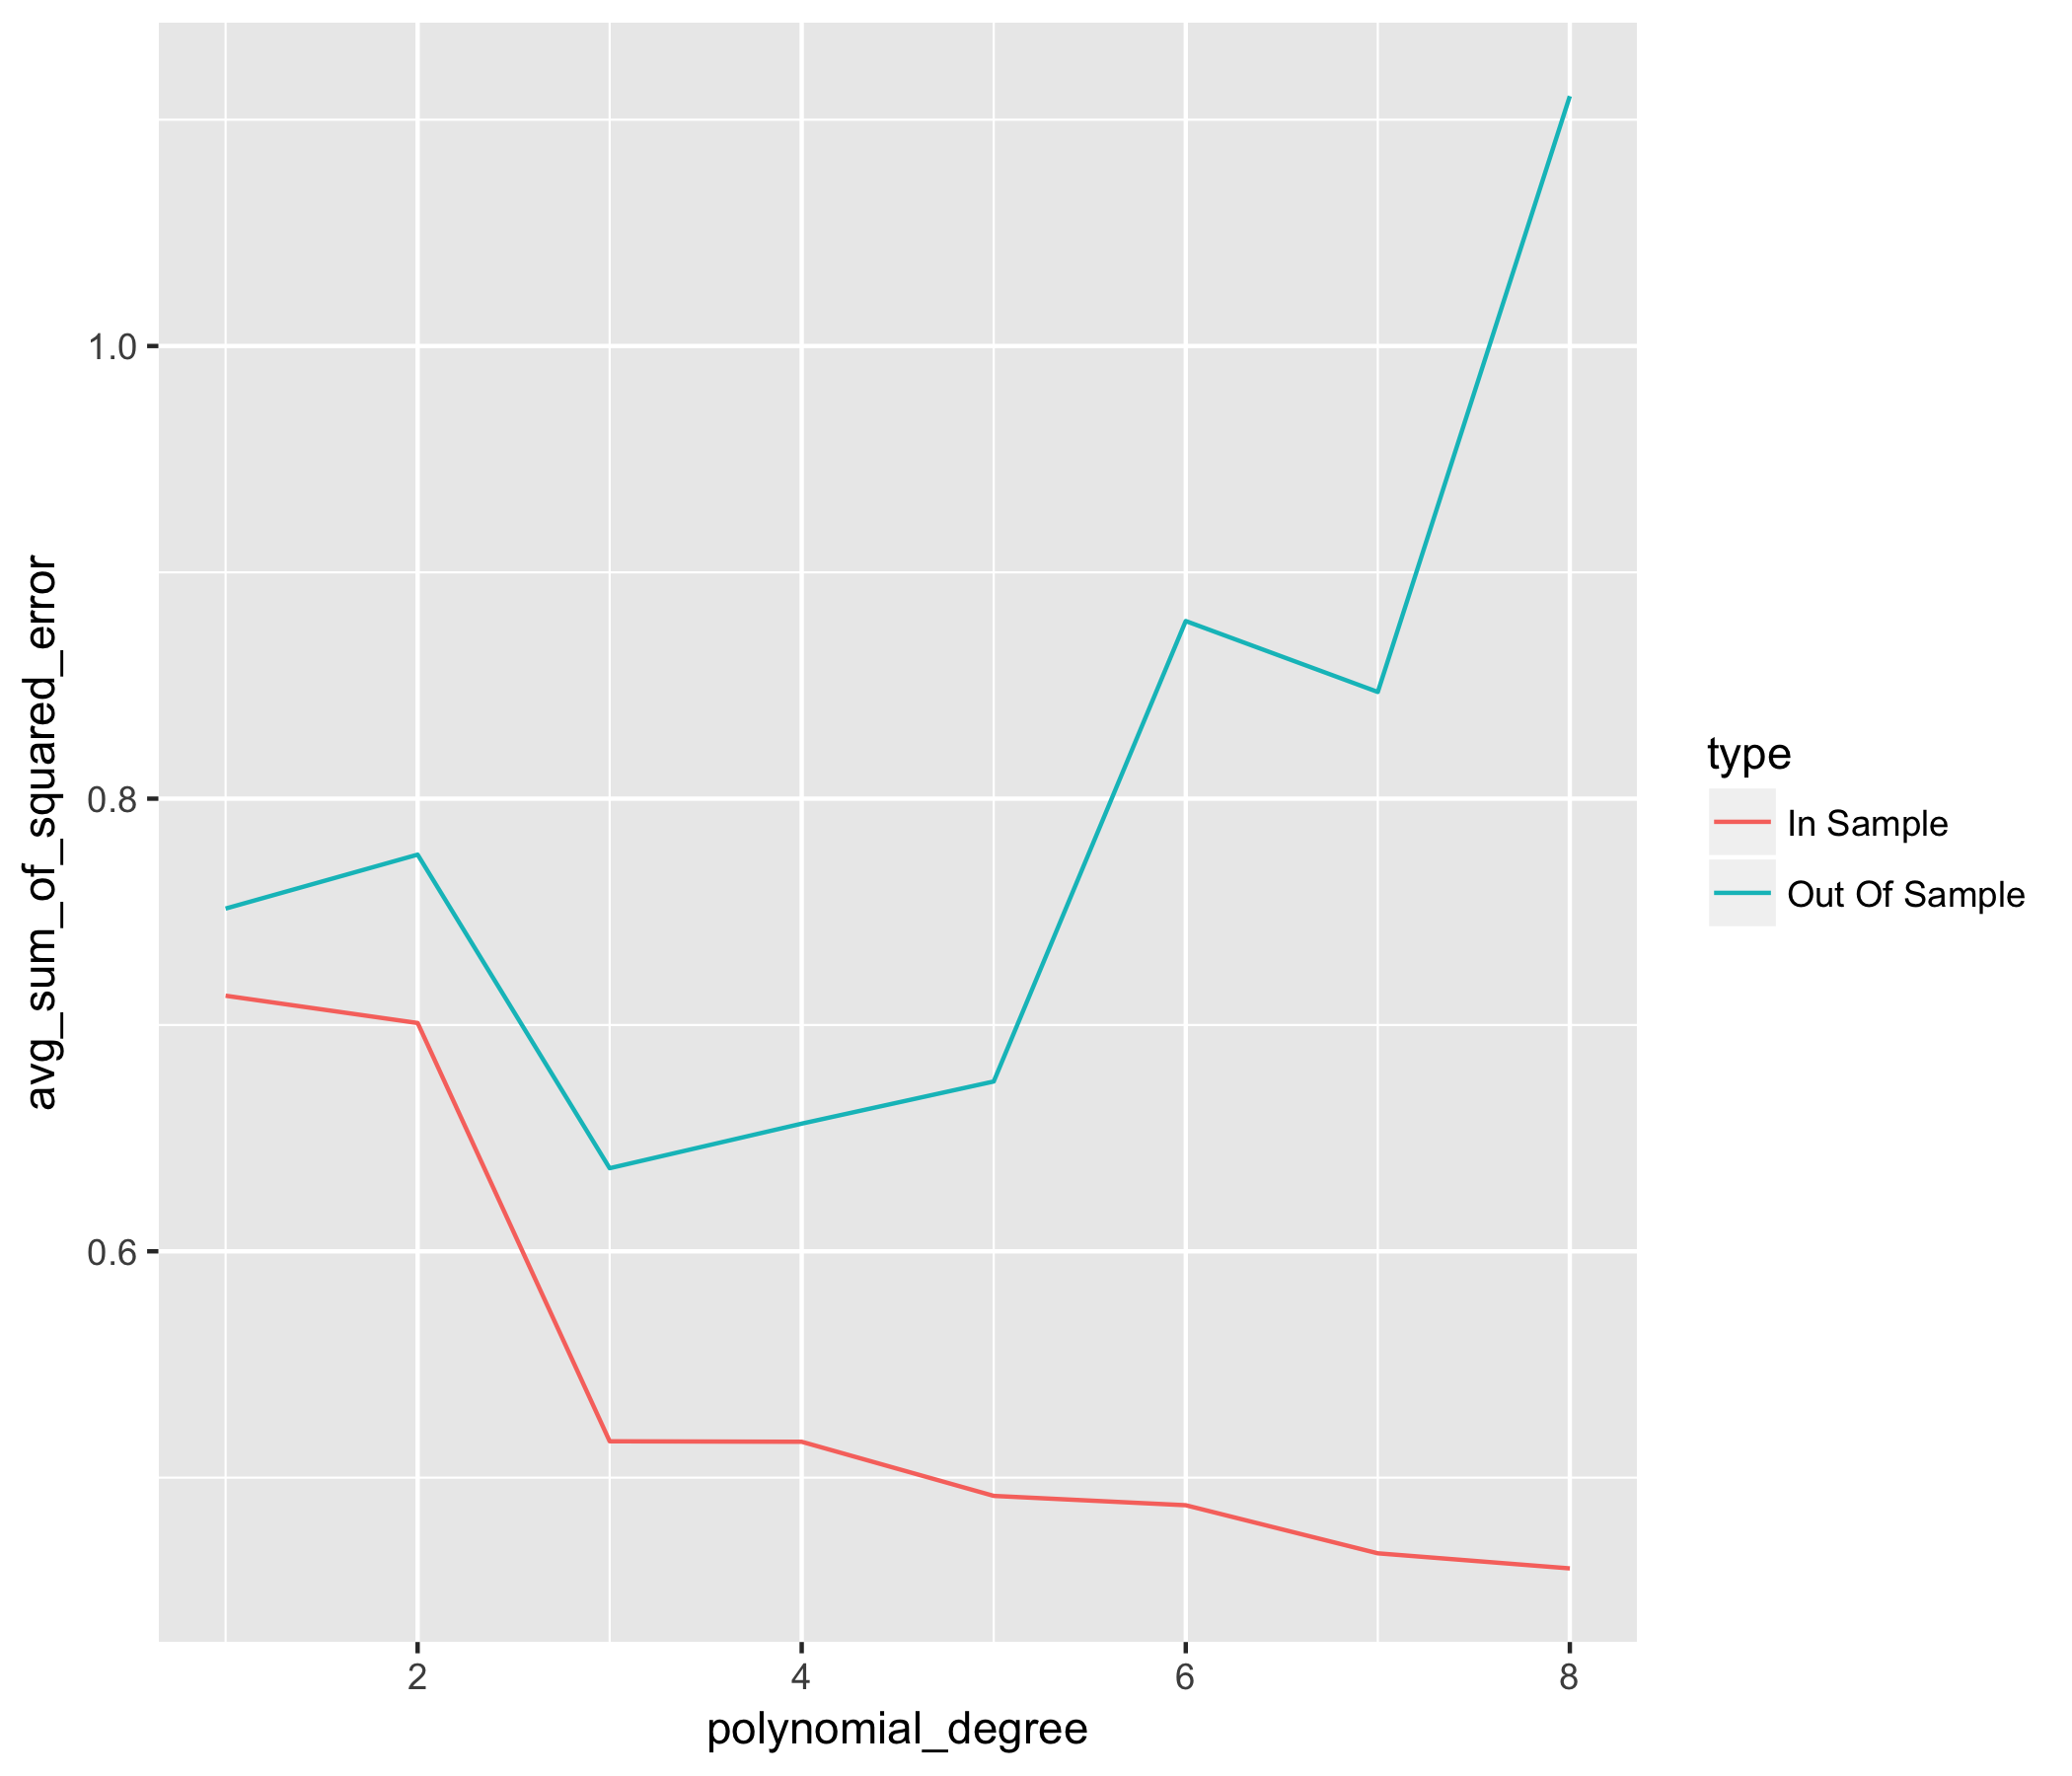
\includegraphics[scale=0.09]{learning_curves_by_degree}
  \end{figure}
  No polynomial curve can capture the true signal completely, but an ideal fit
  is closer the higher the degree.  None-the-less, the decrease in bias is
  overcome by the increase in variance.
\end{frame}

 % A Toy Model
\section{The Out of Sample Error Rate}
%
%
\begin{frame}
  The goal in building a predictive model is often to find an
  appropriate functional form that minimizes the expected error
  rate:
  $$\ESE(f) = E \left[ \left( y - f(x) \right)^2 \right]$$
\end{frame}
%
%
\begin{frame}
  In this section, we turn our attention to estimating this quantity.
\end{frame}
%
%
\begin{frame}
  The first difficulty is that there are different ways to interpret the error,
  depending on what is or is not considered at random.
\end{frame}
%
%
\begin{frame}
  We have already discussed the error when randomizing over both a training set
  and an out of training sample, called the \textbf{expected out of sample
  error}:

  $$\ESE = E_{X,Y,\D} \left[ \left( y - f(x; \D) \right)^2 \right]$$

  It is this quantity that we were able to decompose with the
  \textbf{bias-varaince} decomposition.
\end{frame}
%
%
\begin{frame}
  Possibly more relevant, is the error when randomizing over an out of training
  sample, but for a \textit{fixed} training set:

  $$\ESE(\T) = E_{X,Y} \left[ \left( y - f(x; \T) \right)^2 \right]$$
\end{frame}
%
%
\begin{frame}
  Also convenient is the \textbf{expected training error}, where the sample error is
  computed on the same dataset used to train the model:

  $$\ETE = E_{\T} \left[ \frac{1}{N} \sum_{x,y \in \T} (y - f(x; \T))^2 \right] $$
\end{frame}
%
%
\begin{frame}
  The expected training error is \textit{not} a good estimator of the expected
  out of sample error, because the modeling algorithm incentives fitting the
  training data as closely as possible:
  \begin{figure}
    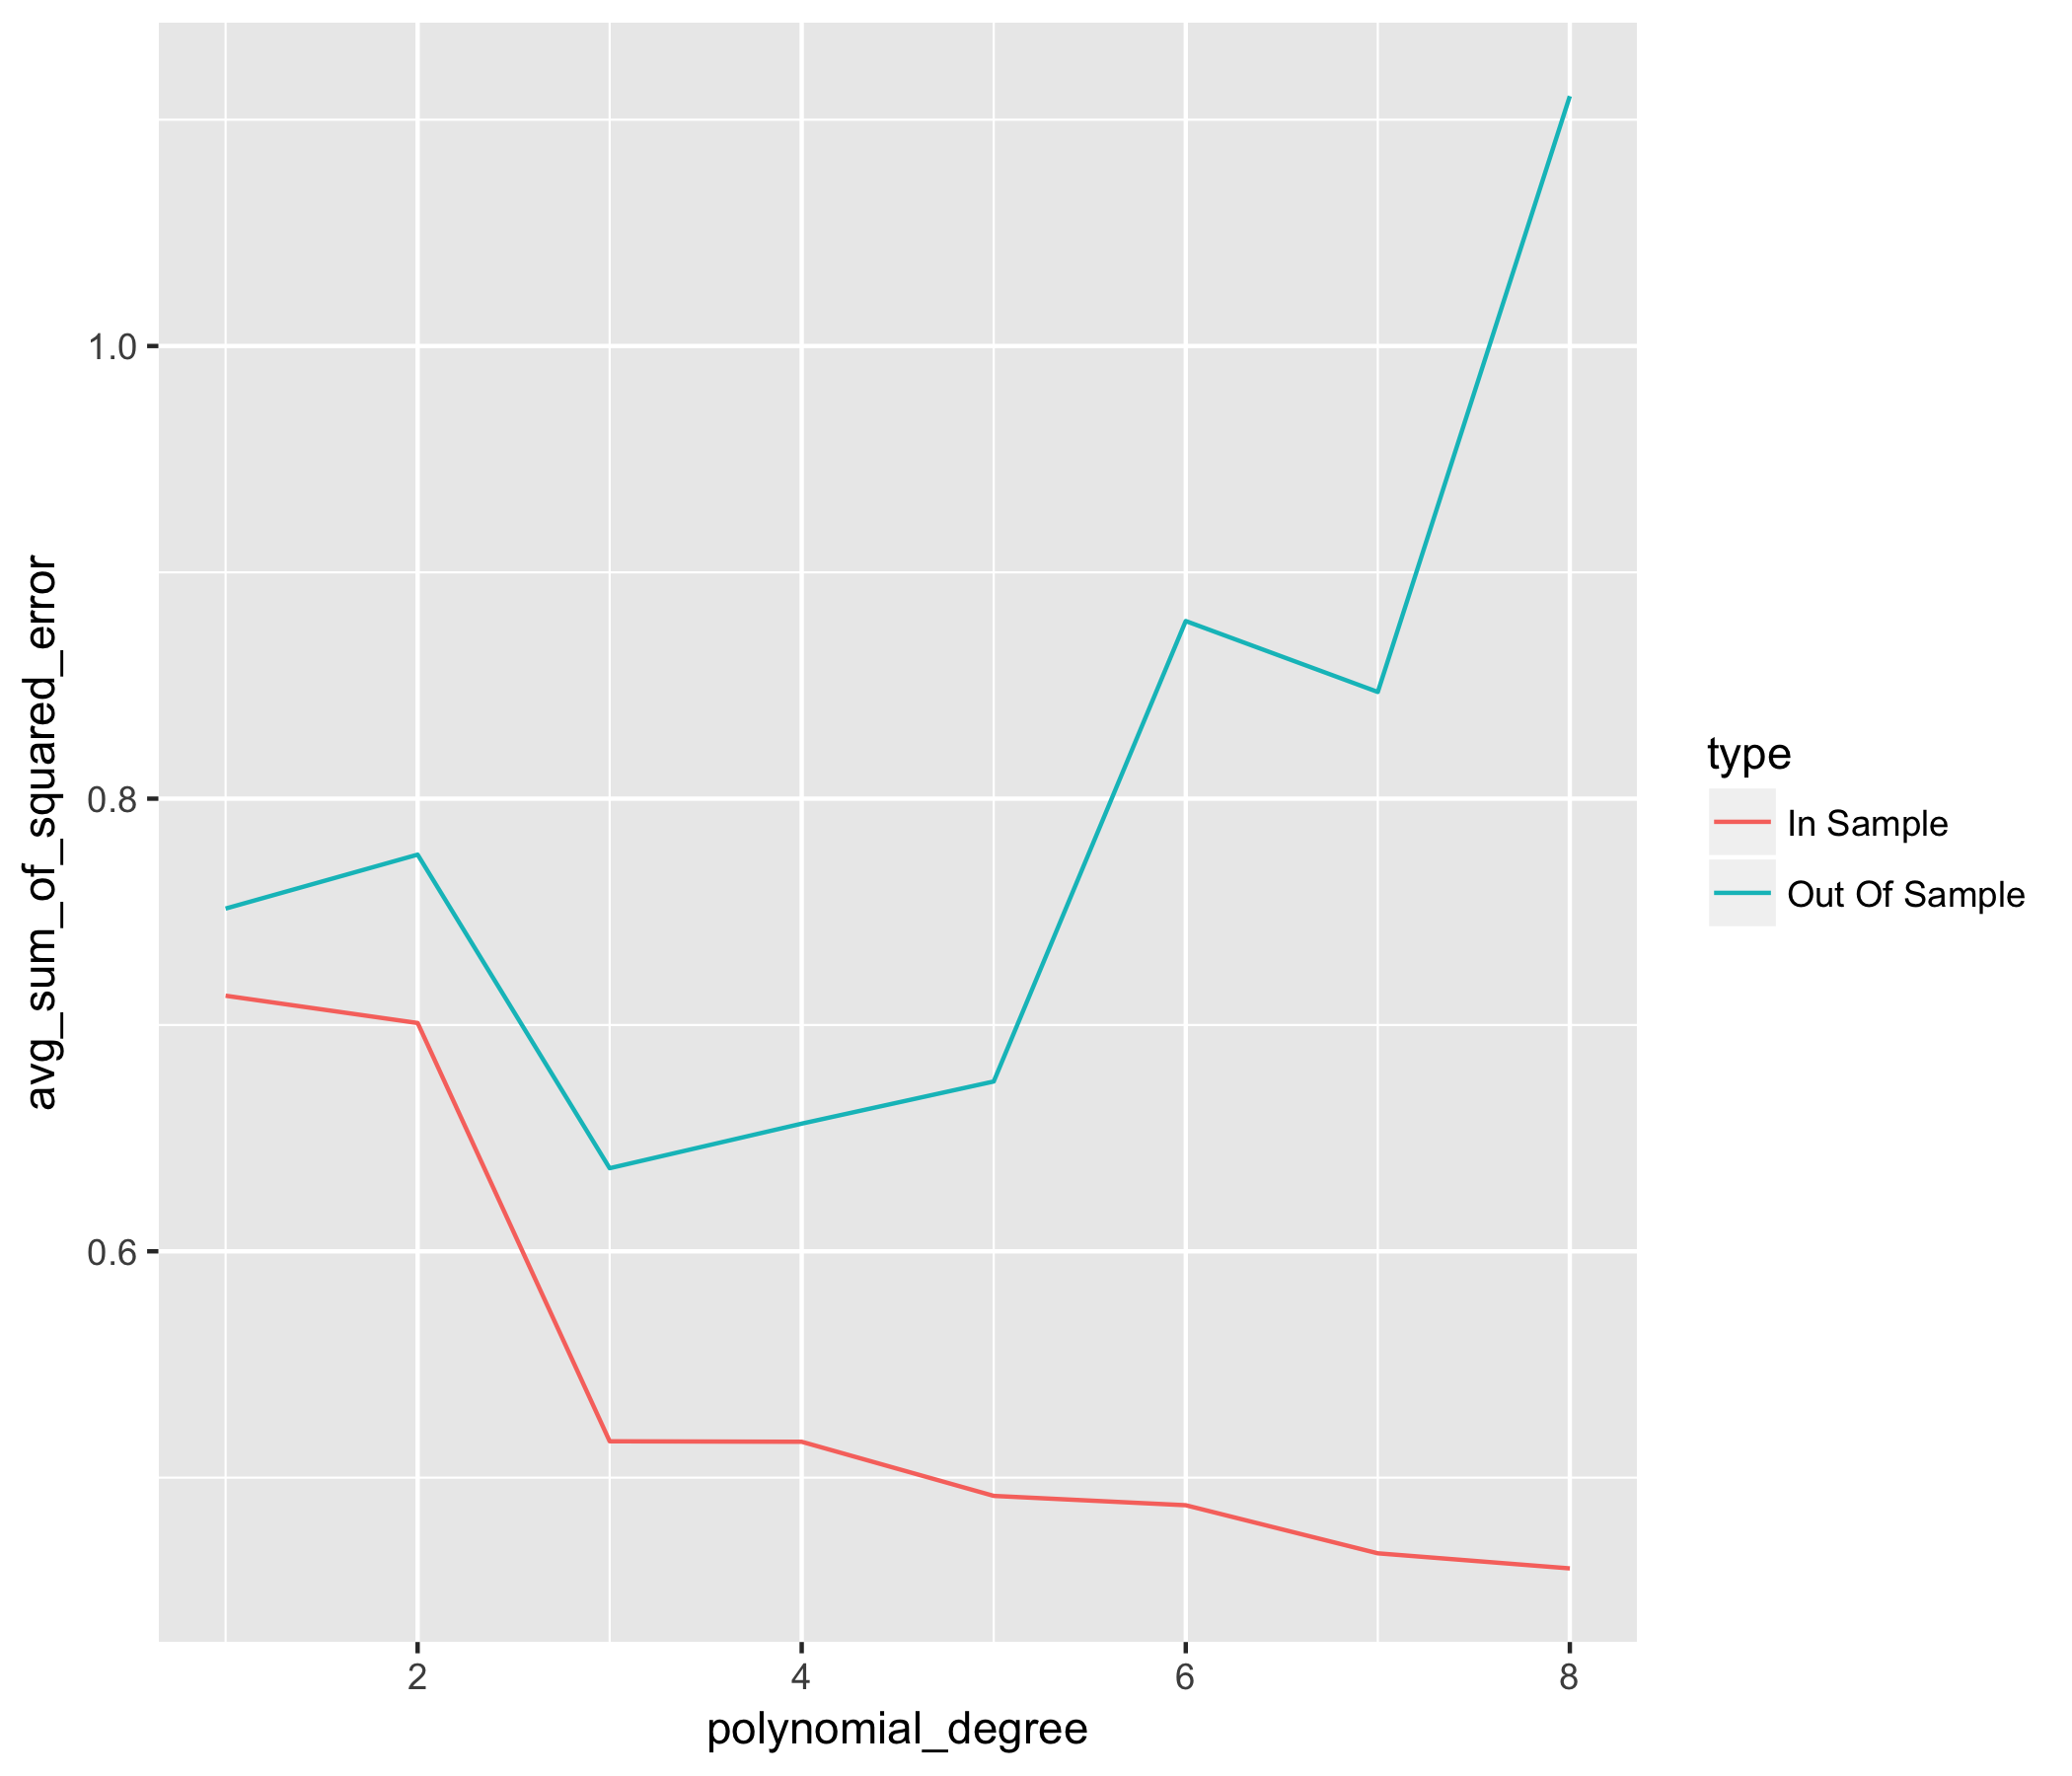
\includegraphics[scale=0.09]{learning_curves_by_degree}
  \end{figure}
\end{frame}
%
%
\begin{frame}
  The effect is amplified in high model variance situations (small data sets or
  noisy data):
  \begin{figure}
    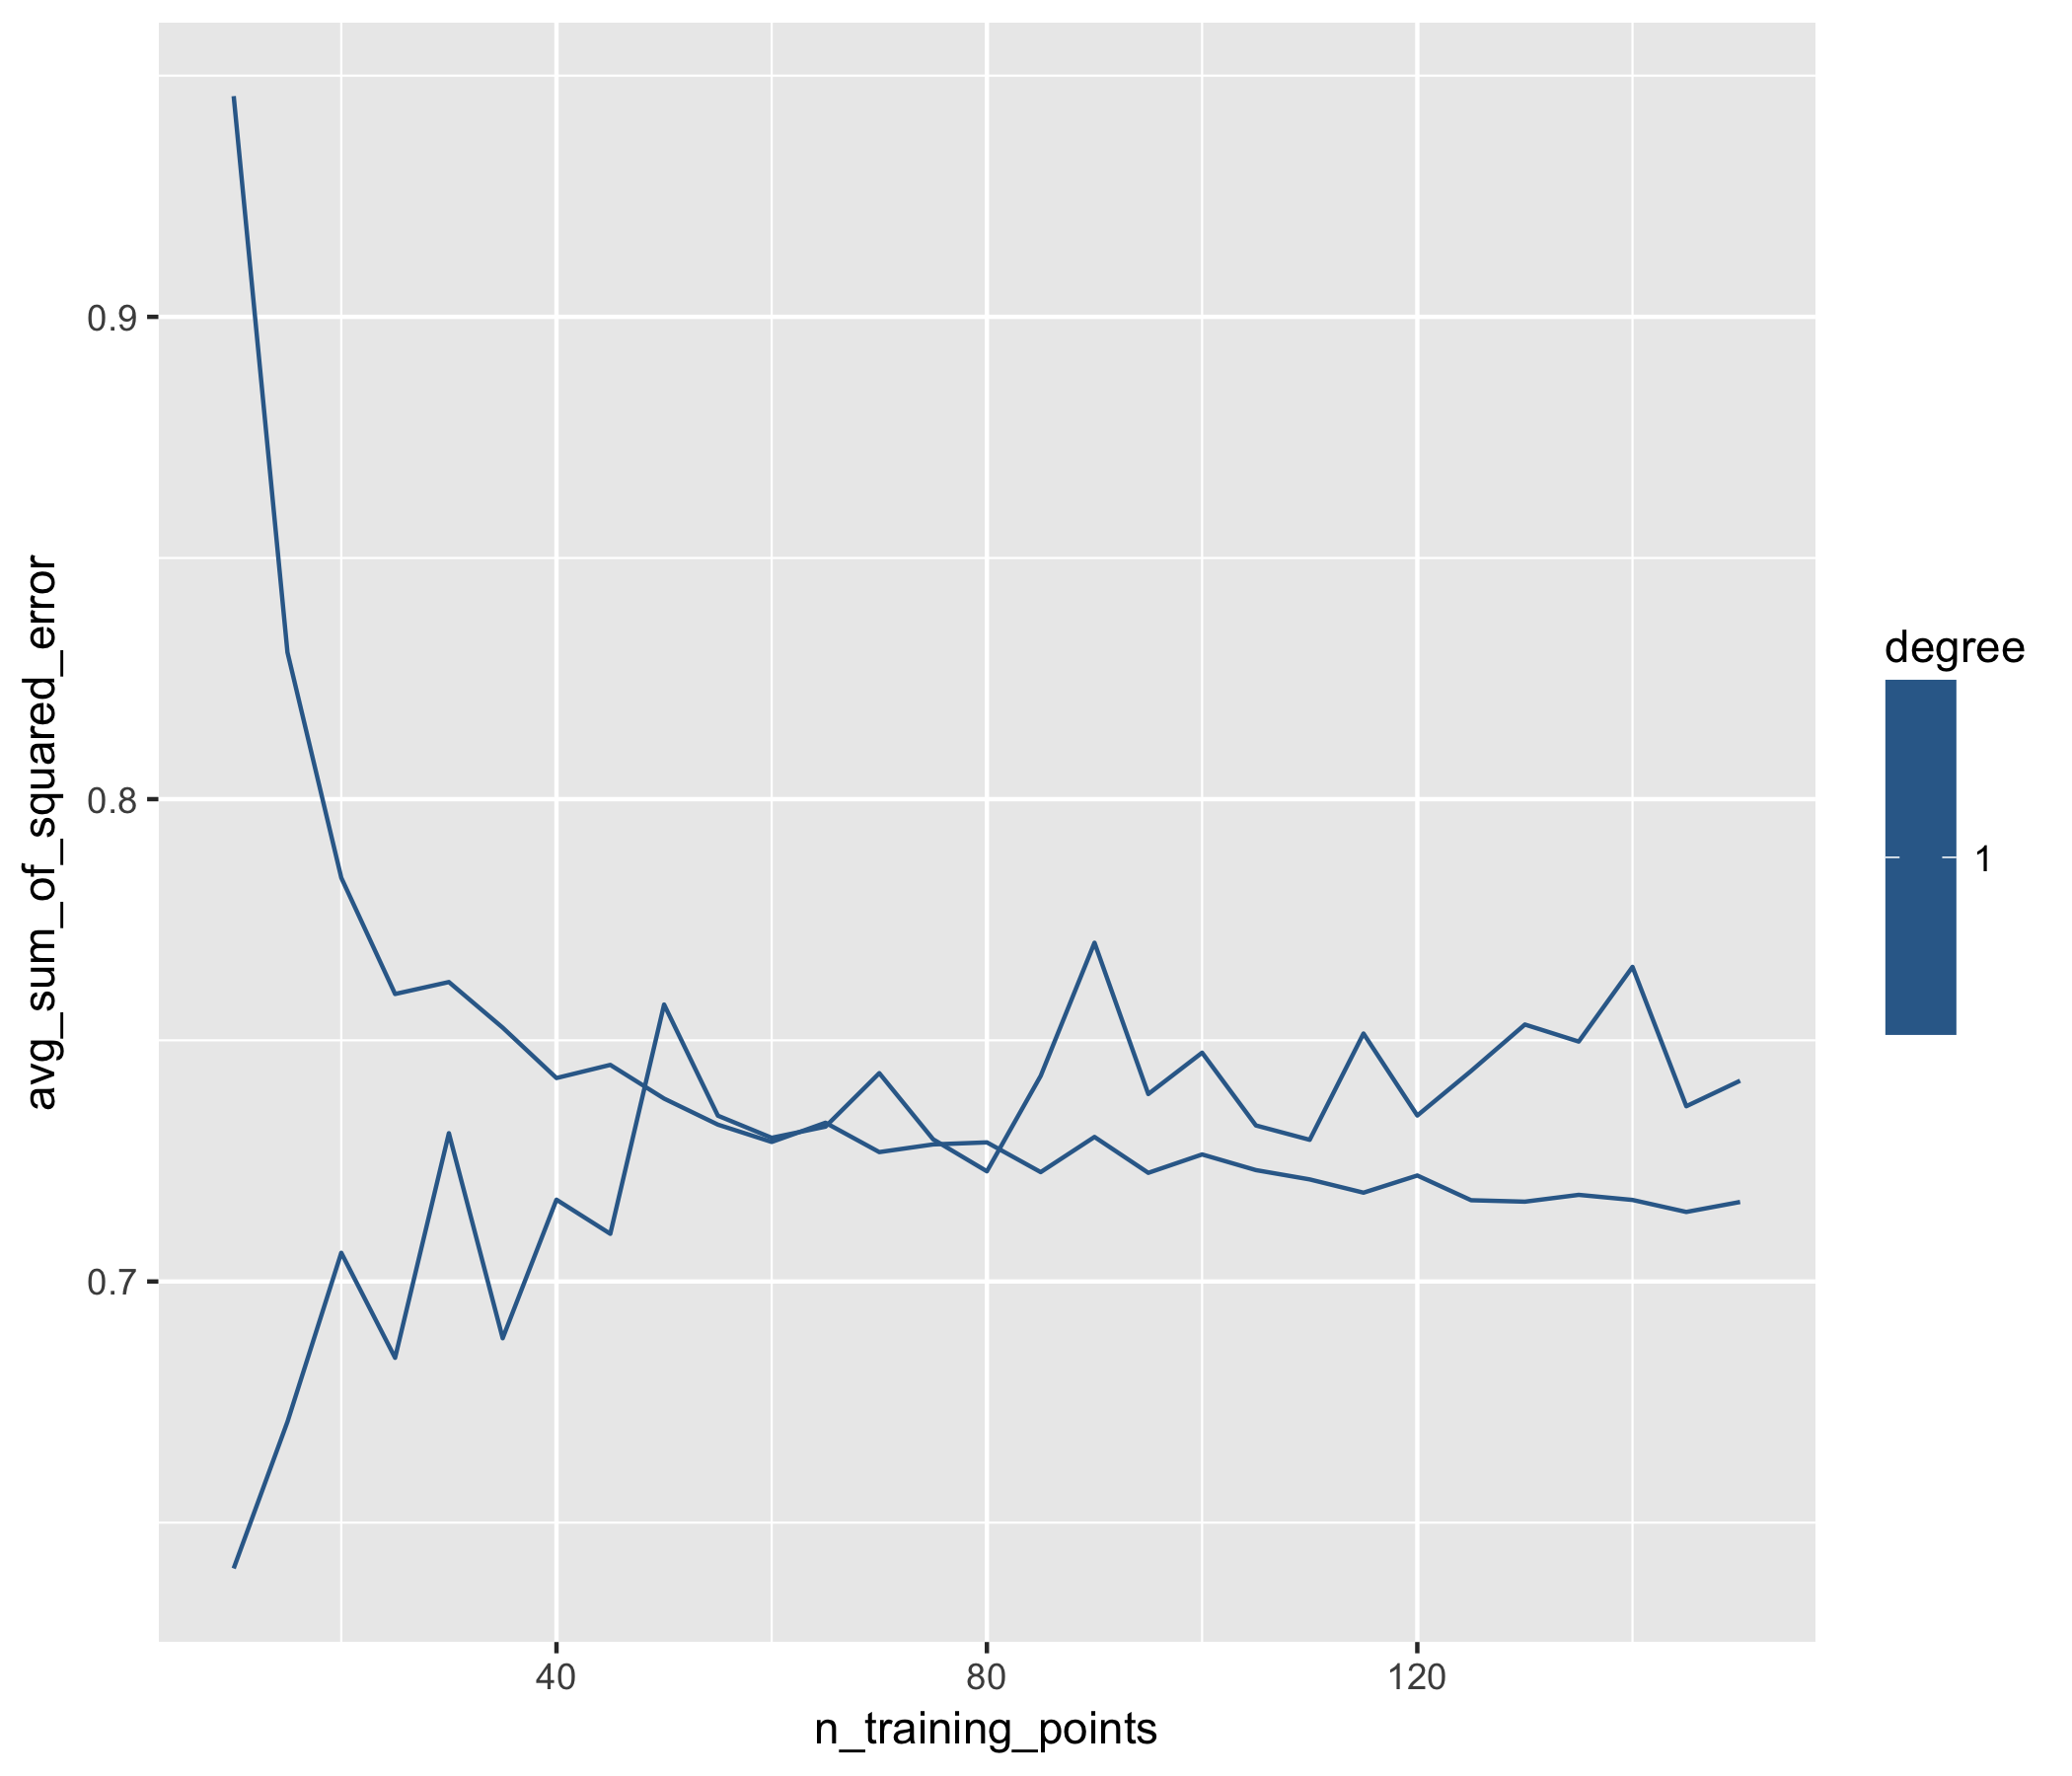
\includegraphics[scale=0.09]{in_and_out_of_sample_learning_curves}
  \end{figure}
\end{frame}
%
%
\begin{frame}
  The bias of the in sample error is so important, it's worth putting some math behind it:
  \begin{align*}
    \ESE &= E_{X,Y,\T} \left[ \left( y - f(x; \T) \right)^2 \right] \\
         \only<2->{
           &= E_{\D, \T} \left[ \frac{1}{N} \sum_{x,y \in \D} (y - f(x; \T))^2
           \right] \\
         }
         \only<3>{
           &\geq E_{\D} \left[ \frac{1}{N} \sum_{x,y \in \D} (y - f(x; \D))^2 \right]
         }
         \only<4>{
           &\geq E_{\T} \left[ \frac{1}{N} \sum_{x,y \in \T} (y - f(x; \T))^2 \right]
         }
  \end{align*}

  \only<2>{
    We can replace the expectation of distribution with the expectation of its
    sample means.
  }
  \only<3>{
    This is the definition of $f(X, \D)$, it has smaller error than all other
    possible $f$ when the sample error is evaluated on $\D$.
  }
  \only<4>{
    Changing the name of a free variable.
  } 
\end{frame}
%
%
\begin{frame}
  Since the training error is not a good estimate of the out of sample error, we
  need an alternative way to get at this quantity.  There are two major
  approaches:
  \begin{itemize}
    \item Using a \textbf{hold out set}.
    \item Using \textbf{cross validation}.
  \end{itemize}
\end{frame}
%
%
\begin{frame}
  If a dataset $\Holdout$ has participated in neither the training of the model, or
  the decision making process, then:

  $$ \frac{1}{N} \sum_{x,y \in \Holdout} (y - f(x; \T))^2 $$

  is an unbias estimate of $\ESE(\T)$ (the expected out of sample error with a
  fixed training set).
\end{frame}
%
%
\begin{frame}
  Holding out data is \textit{not} costless, as there is less data available for
  training and a smaller data set will increase the variance of the estimated
  model:
  \begin{figure}
    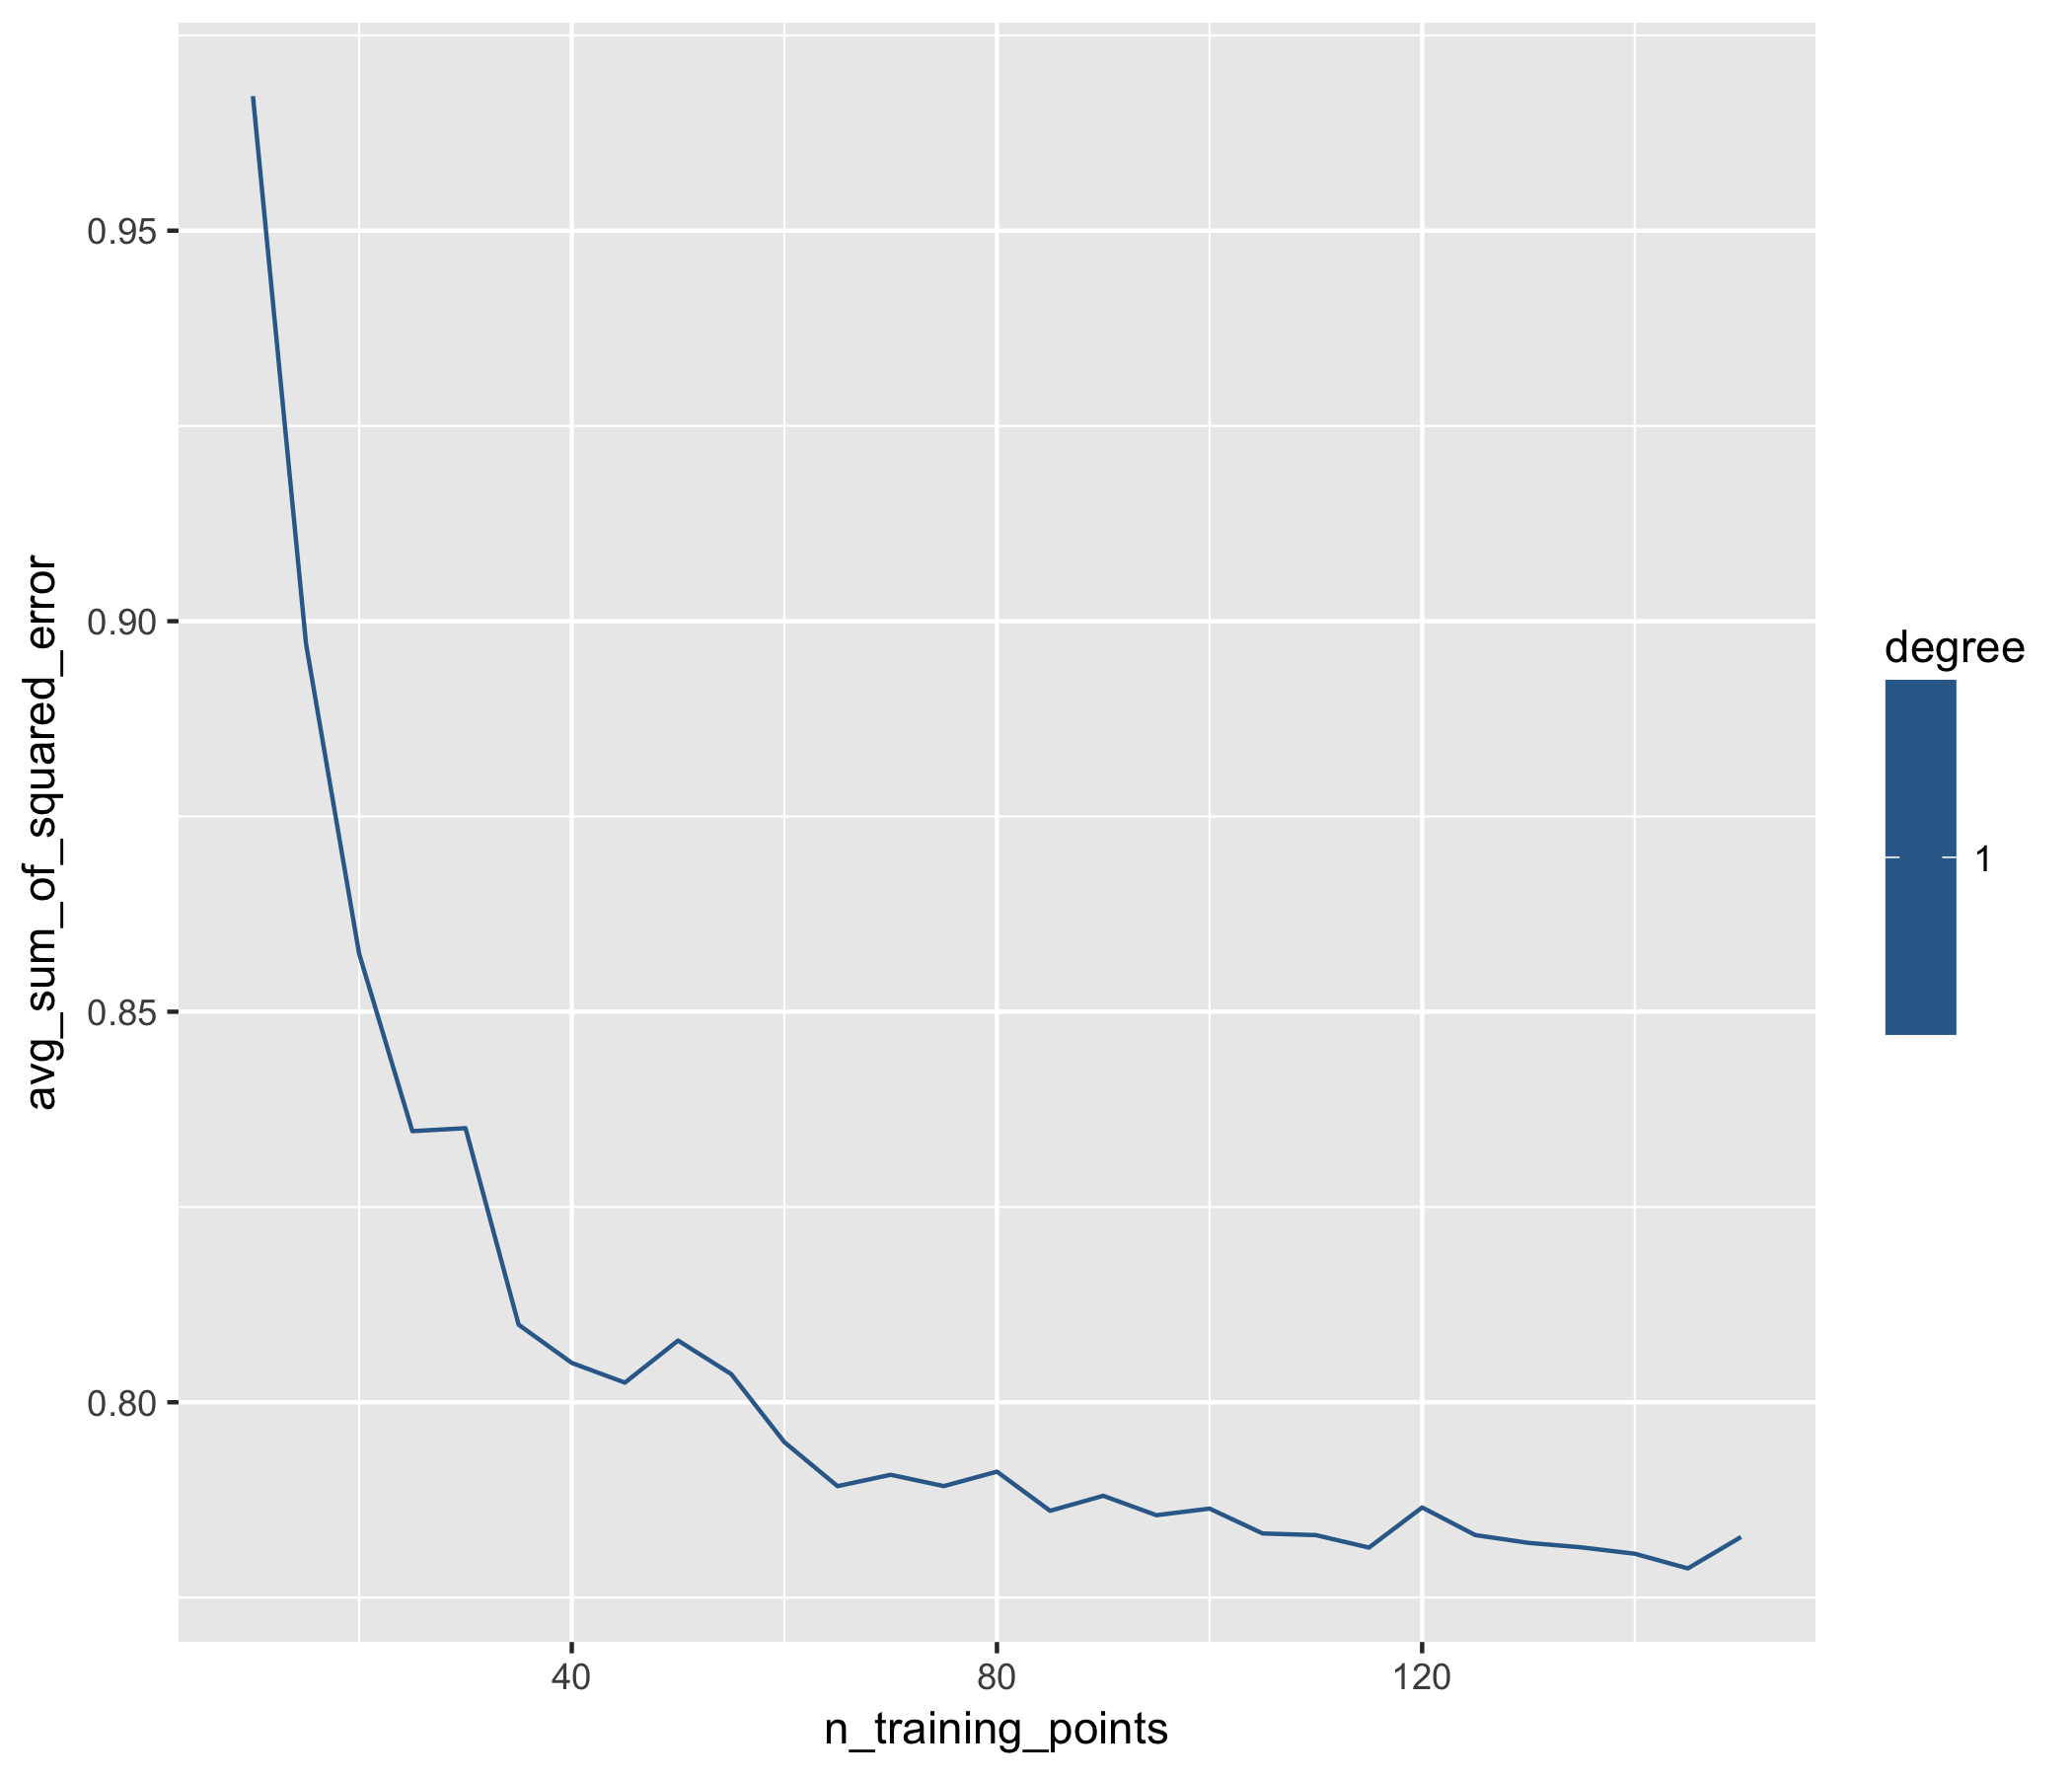
\includegraphics[scale=0.08]{out_of_sample_learning_curve}
  \end{figure}
  How costly holding out data is depends on the shape of the learning curve for
  the model being estimated.
\end{frame}
%
%
\begin{frame}
  \begin{figure}
    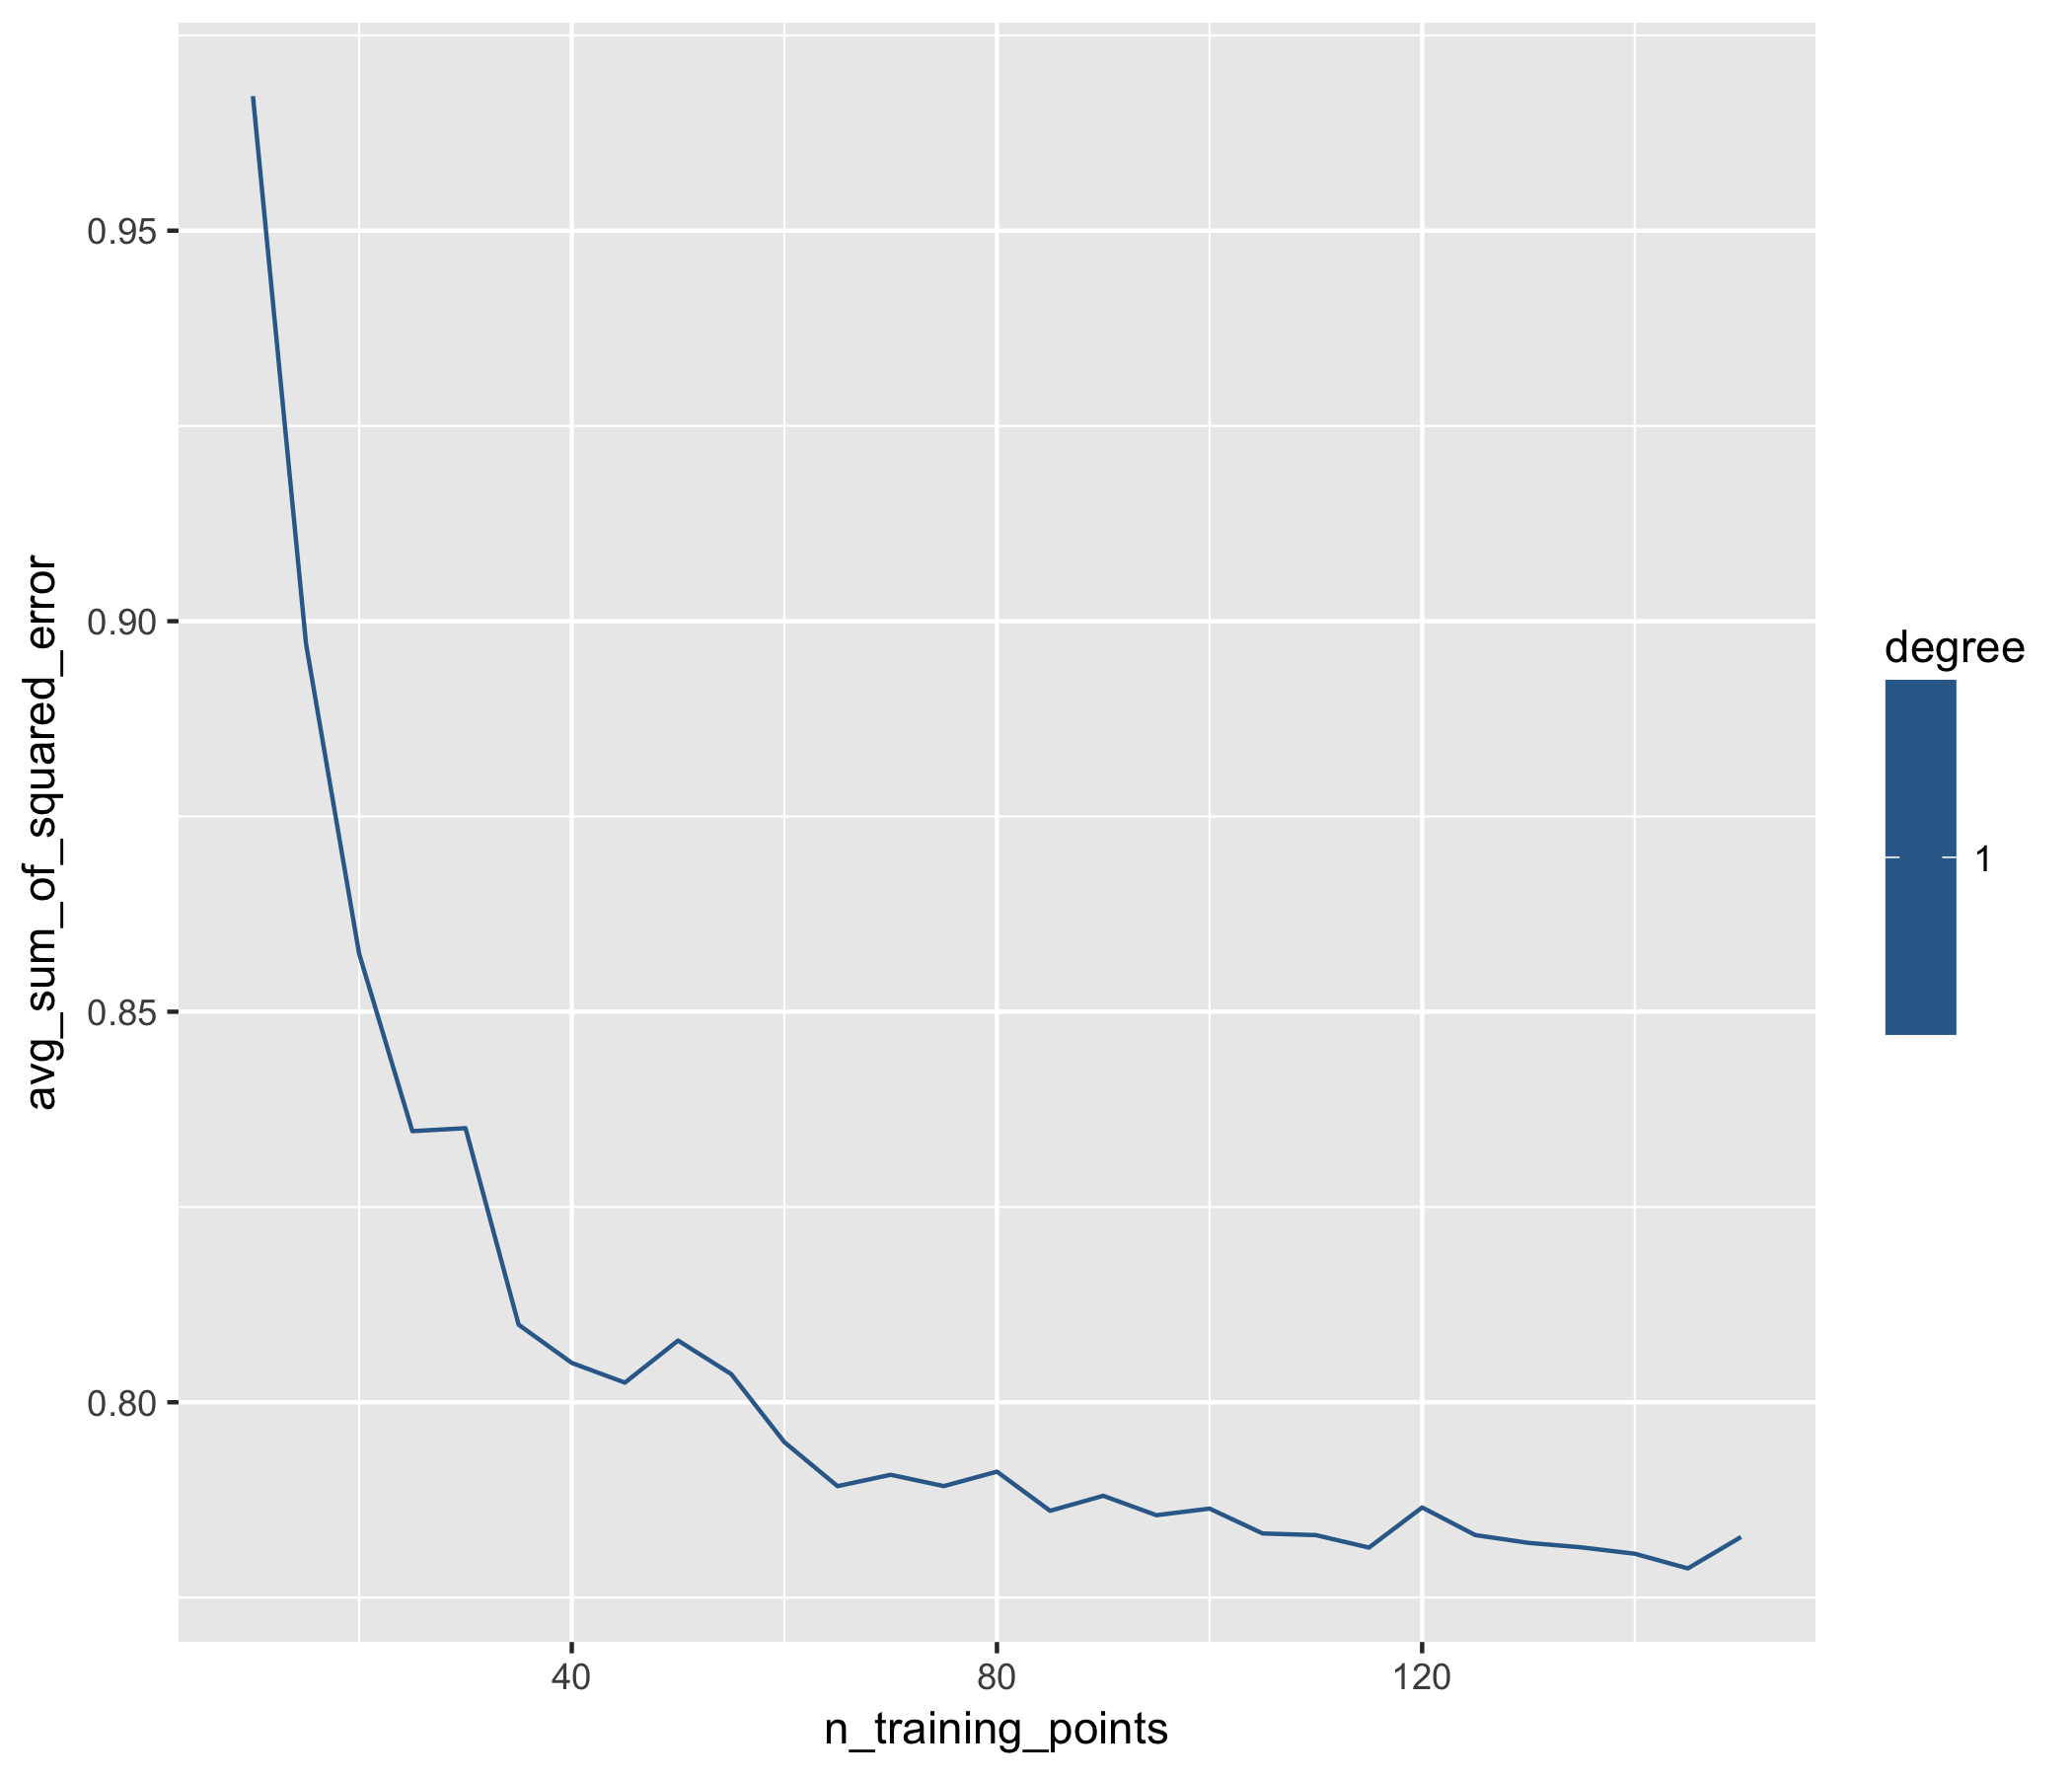
\includegraphics[scale=0.08]{out_of_sample_learning_curve}
  \end{figure}
  This shape is affected by:
  \begin{itemize}
    \item The overall level of noise in the data (irreducible error).
    \item The complexity of the model being estimated.
  \end{itemize}
  Noisier data and more complex models may be more adversely affected by holding
  out data.
\end{frame}
%
%
\begin{frame}
  In \textbf{cross validation} the data is available is partitioned into a
  disjoint union of \textit{folds}:
  $$ {\T} = {\T}_1 \cup {\T}_2 \cup \cdots \cup {\T}_k $$
  For each $i$, the out of fold data is formed by removing the fold ${\T}_i$ from
  the training data set:
  $$ \hat{{\T}}_i = {\T}_1 \cup \cdots \cup {\T}_{i-1} \cup {\T}_{i+1}
  \cup \cdots \cup {\T}_k $$
\end{frame}
%
%
\begin{frame}
  The cross validation estimate of the out of sample error is:
   $$ \frac{1}{k} \sum_{i=1}^{k} \frac{1}{\# {\T}_i } \sum_{x,y \in
   {\T}_i} (y - f(x, \hat{{\T}}_i))^2$$ 
   Since we are randomizing over a training set, this is actually an estimate of
   $\ESE$.
\end{frame}
%
%
\begin{frame}
  That is, while the hold out sample error is an estimate of:
  $$\ESE(\T) = E_{X,Y} \left[ \left( y - f(x; \T) \right)^2 \right]$$
  The cross validation estimate is of:
  $$\ESE = E_{X,Y,\D} \left[ \left( y - f(x; D) \right)^2 \right]$$
\end{frame}
%
%
\begin{frame}
  The number of folds to use is yet another example of balance and compromise in
  statistical modeling.
\end{frame}
%
%
\begin{frame}
  If a small $k$ is chosen, much data is held out from each training set,
  depending on how much total data is available, this can increase the variance
  of the estimated model:
  \begin{figure}
    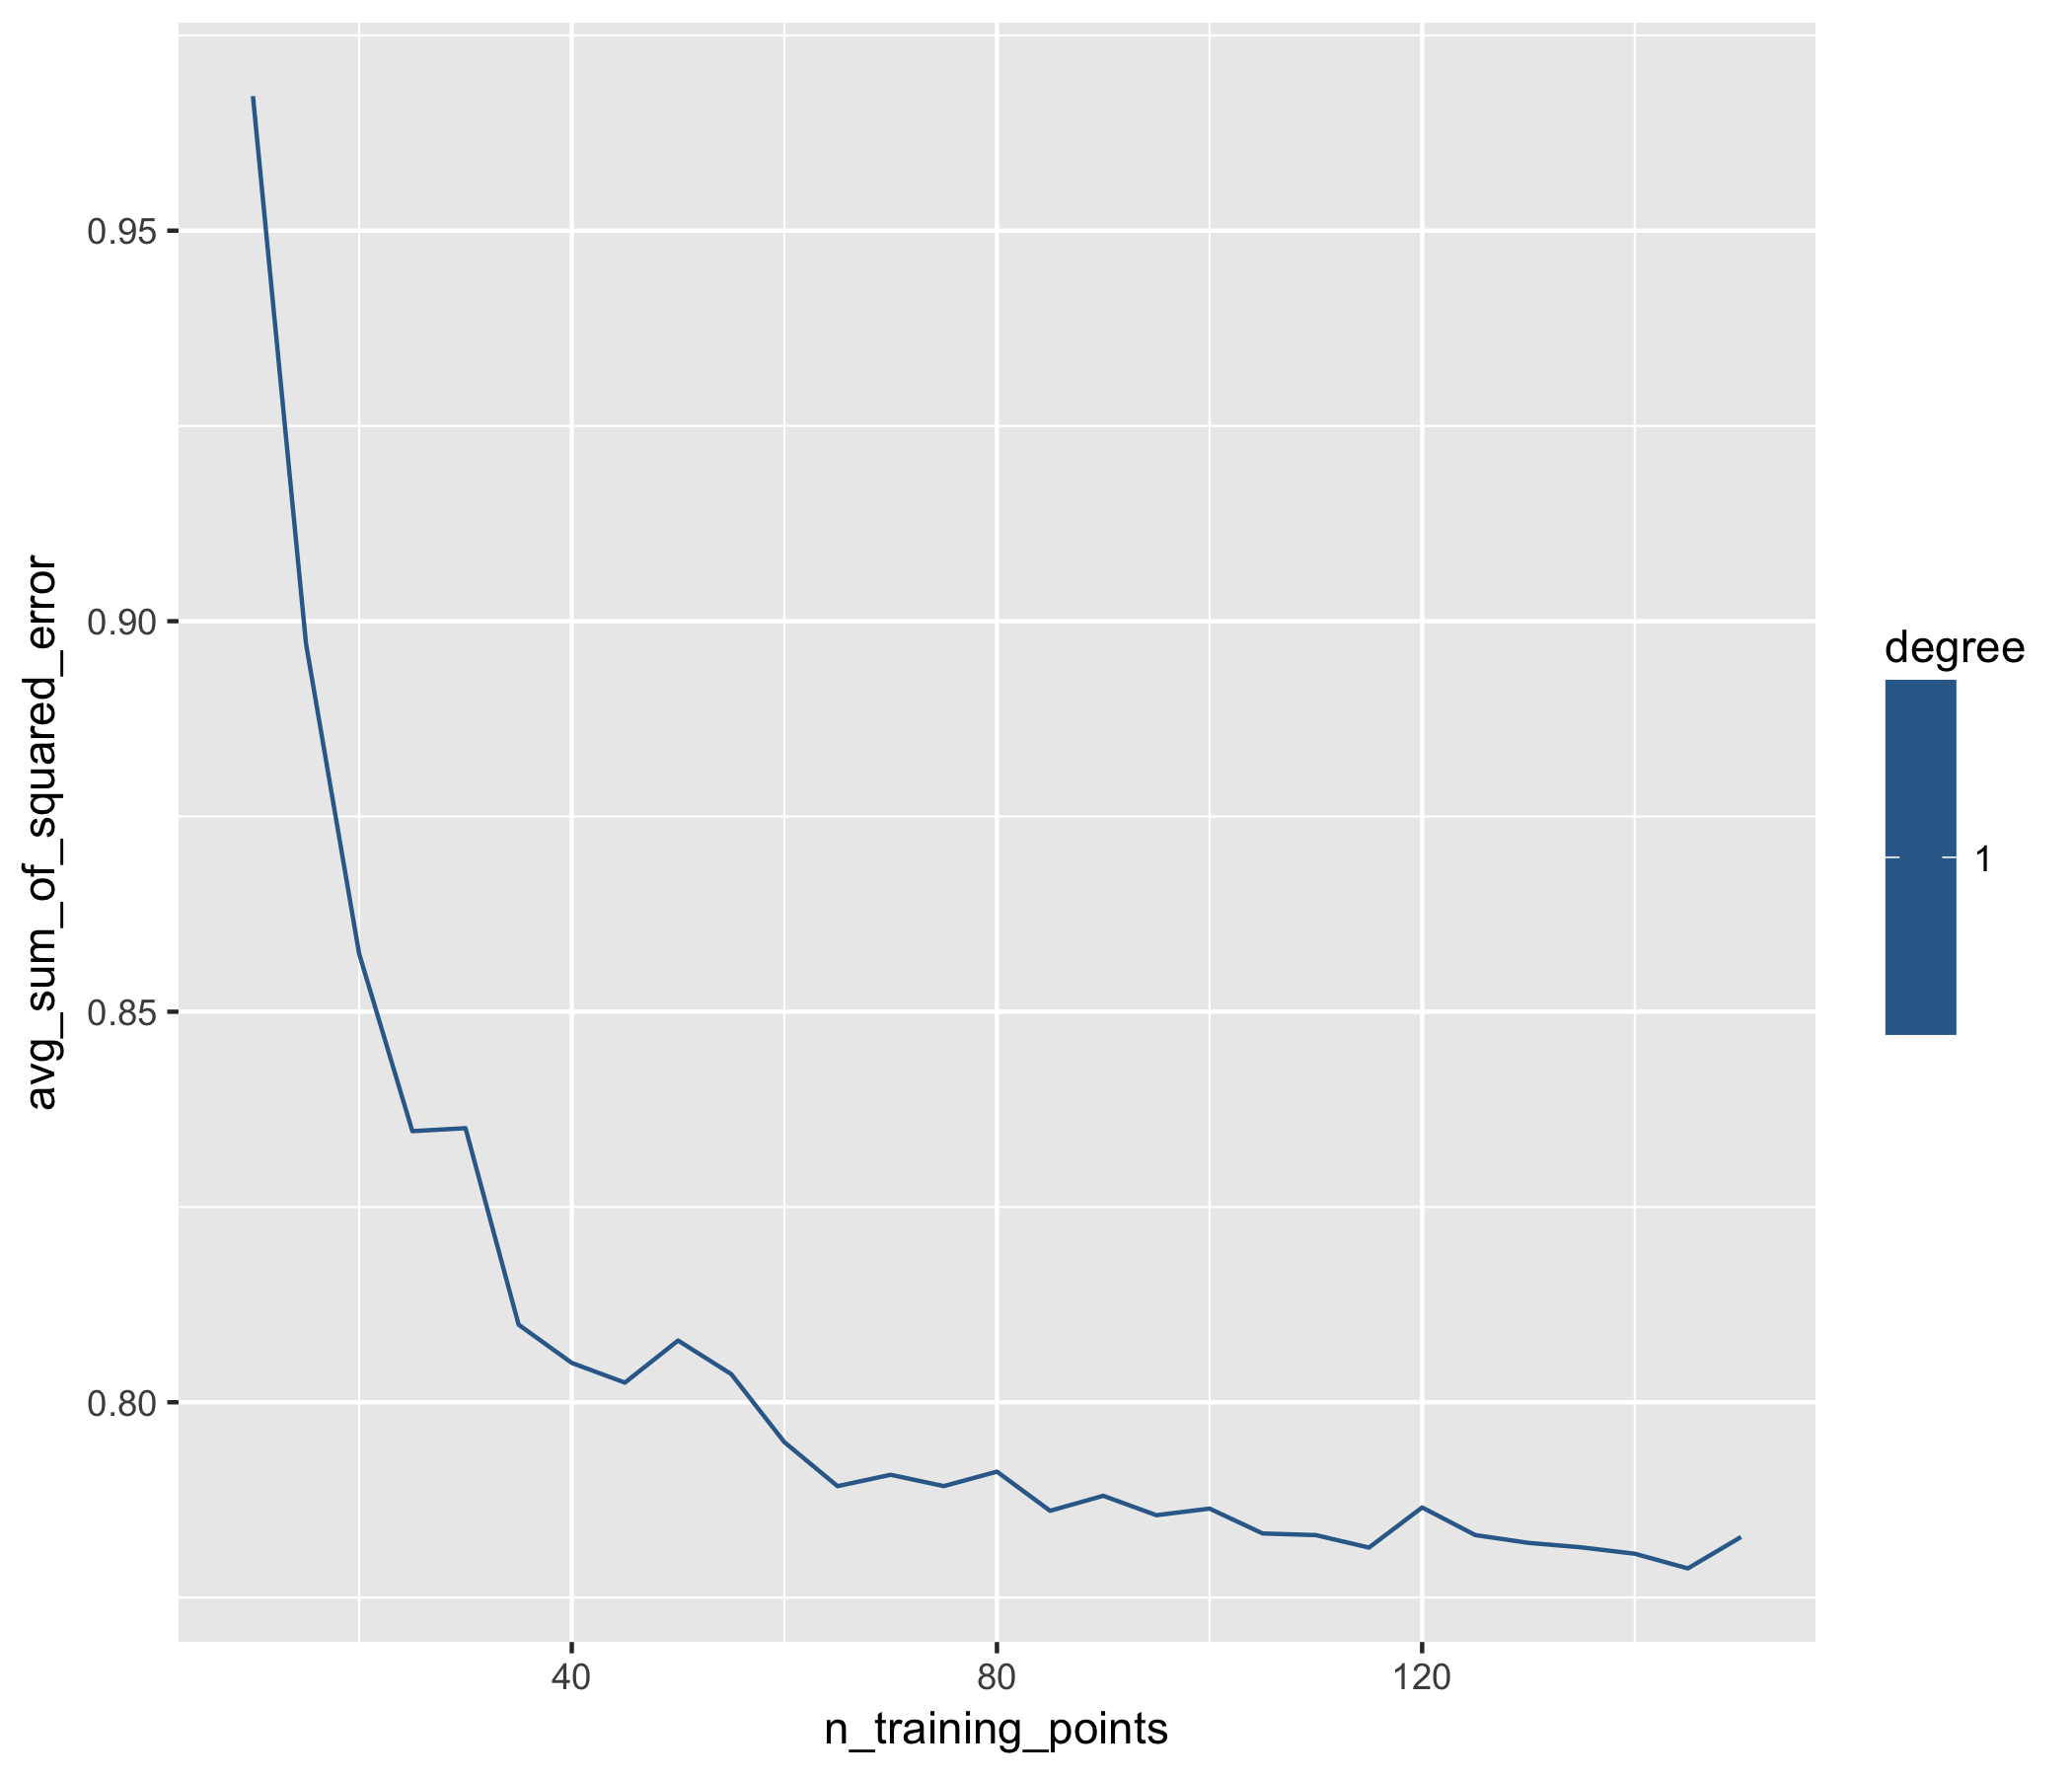
\includegraphics[scale=0.09]{out_of_sample_learning_curve}
  \end{figure}
\end{frame}
%
%
\begin{frame}
  At the other extreme, the $k = N$ case is called \textbf{leave one out cross
  validation}.  In this case the models trained on the complementary sets are
  highly correlated, as the various training sets differ at only one point:

  $$ f(x, \hat{{\T}}_i) \approx  f(x, \hat{{\T}}_j) $$
\end{frame}
%
%
\begin{frame}
  This makes the cross validation estimator relatively insensitive to model
  variance, as the training data is not sufficiently averaged out.

  Said another way, if the cross validation estimate is repeated over various
  \textit{full} training sets, \textit{this estimate} will have high variance.
\end{frame}
 % Out of Sample Error Rate
%
\end{document}
